\documentclass[11pt]{book}

% Set table of contents depth

\setcounter{tocdepth}{2}

% Set the margins

\usepackage[left=3.5cm,top=3.5cm,right=2.5cm,bottom=3.0cm,a4paper,twoside]{geometry}

% Set one-and-a-half spacing

\usepackage{setspace}
\setstretch{1.5}

% Set font to charter (just remove for default font)

\usepackage[charter]{mathdesign}

% Set chapter style to avantgarde (big grey numbers)
\usepackage{xcolor}
\RequirePackage[avantgarde]{quotchap}

% Load various packages

\usepackage{natbib}
\usepackage{graphicx}
\usepackage{xspace}
\usepackage{lscape}
\usepackage{longtable}
\usepackage{amsmath}
\usepackage{fancyhdr}
\usepackage{titlesec}
\usepackage[breaklinks]{hyperref}
\usepackage{afterpage}
\usepackage[hang,flushmargin]{footmisc} 
\usepackage{todonotes}
\usepackage{epigraph}

% Adding packages for epigraphs.
\setlength\epigraphwidth{1\textwidth}
\setlength\epigraphrule{0pt} % no line between
\setlength\beforeepigraphskip{1\baselineskip} % space before and after epigraph
\setlength\afterepigraphskip{2\baselineskip}
\renewcommand*{\textflush}{flushright}
\renewcommand*{\epigraphsize}{\normalsize\itshape}

% Set caption style

\usepackage[small,bf]{caption}

% Include custom definitions (edit definitions.tex)

\usepackage{xspace}

\newcommand{\eq}{Eq.}
\newcommand{\eqs}{Eqs.}
\newcommand{\fig}{Figure}
\newcommand{\figs}{Figures}

\newcommand{\figshortleft}{{\textit{left}}}
\newcommand{\figshortcenter}{{\textit{center}}}
\newcommand{\figshortright}{{\textit{right}}}

\newcommand{\figleft}{{\textit{Left}}~--~}
\newcommand{\figcenter}{{\textit{Centre}}~--~}
\newcommand{\figright}{{\textit{Right}}~--~}

\newcommand{\figtopleft}{{\textit{Top left}}~--~}
\newcommand{\figtopright}{{\textit{Top right}}~--~}

\newcommand{\figcenterleft}{{\textit{Centre left}}~--~}
\newcommand{\figcenterright}{{\textit{Centre right}}~--~}

\newcommand{\figbottom}{{\textit{Bottom}}~--~}
\newcommand{\figtop}{{\textit{Top}}~--~}

\newcommand{\figbottomleft}{{\textit{Bottom left}}~--~}
\newcommand{\figbottomright}{{\textit{Bottom right}}~--~}

%%%%%%%%%%%%%%%%% Abbreviations %%%%%%%%%%%%%%%%%

\newcommand\tablenotemark[1]{$^{\rm #1}$\xspace}
\newcommand\nodata{$\cdots$}
%----------------- Parameters -------------------

%\newcommand\ion[2]{#1$\;${\small\rmfamily\@Roman{#2}}\relax}%
\renewcommand\line[2]{#1$\;${\small\sc #2}\xspace}%
\newcommand\forbidden[2]{[#1$\;${\small\sc #2}]\xspace}%

%% MATH SYMBOLS %%

\newcommand{\agestar}{t_{\star}}

\newcommand{\mstar}{M_{\star}}
\newcommand{\rstar}{R_{\star}}
\newcommand{\tstar}{T_{\star}}

\newcommand{\mdote}{\dot{M}_{\rm env}}
\newcommand{\rmaxe}{R_{\rm env}^{\rm max}}
\newcommand{\rmine}{R_{\rm env}^{\rm min}}

\newcommand{\mdisk}{M_{\rm disk}}
\newcommand{\mdotdisk}{\dot{M}_{\rm disk}}

\newcommand{\rmaxd}{R_{\rm disk}^{\rm max}}
\newcommand{\rmind}{R_{\rm disk}^{\rm min}}

\newcommand{\rsub}{R_{\rm sub}}

\newcommand{\rhoconst}{\rho_{\rm cavity}}
\newcommand{\thetacav}{\theta_{\rm cavity}}

\newcommand{\rhoamb}{\rho_{\rm ambient}}

\newcommand{\rc}{R_{\rm c}}

\newcommand{\zmin}{z_{\rm factor}}

\newcommand{\msunmath}{M_{\odot}}

\newcommand{\renv}{R_{\rm{env}}}

\newcommand{\fnu}{F_{\nu}}
\newcommand{\rnu}{R_{\nu}}
\newcommand{\fnua}{F_{\nu}{\rm{[actual]}}}
\newcommand{\fnuq}{F_{\nu}{\rm{[assumed]}}}
\newcommand{\fnuqz}{F_{\nu_0}{\rm{[quoted]}}}
\newcommand{\fnuqiso}{F_{\nu_0}^{\rm iso}{\rm{[quoted]}}}

%% UNITS %%

% Temperature

\newcommand{\kelvin}{\,K\xspace}

% Distance

\newcommand{\angstrom}{\,\AA\xspace}
\newcommand{\microns}{\,$\mu$m\xspace}
\newcommand{\mm}{\,mm\xspace}
\newcommand{\rsun}{$R_{\odot}$\xspace}
\newcommand{\au}{\,AU\xspace}
\newcommand{\pc}{\,pc\xspace}
\newcommand{\kpc}{\,kpc\xspace}
\newcommand{\cm}{\,cm\xspace}
\newcommand{\m}{\,m\xspace}

% Time

\newcommand{\seconds}{\,s\xspace}
\newcommand{\days}{\,days\xspace}
\newcommand{\yr}{\,yr\xspace}
\newcommand{\peryr}{\,yr$^{-1}$\xspace}
\newcommand{\Myr}{\,Myr\xspace}
\newcommand{\perMyr}{\,Myr$^{-1}$\xspace}

% Mass

\newcommand{\msun}{\,$M_{\odot}$\xspace}
\newcommand{\msunperyr}{\,$M_{\odot}$\,yr$^{-1}$\xspace}

% Luminosity/Brightness

\newcommand{\lsun}{$L_{\odot}$\xspace}
\newcommand{\mags}{\,mag\xspace}
\newcommand{\Jy}{\,Jy\xspace}
\newcommand{\mJy}{\,mJy\xspace}
\newcommand{\MJysr}{\,MJy/sr\xspace}

% Other

\newcommand{\arcsec}{$^{\prime\prime}$\xspace}
\newcommand{\arcmin}{$^{\prime}$\xspace}
\newcommand{\degrees}{$^\circ$\xspace}
\newcommand{\sqdeg}{\,deg$^2$\xspace}

\newcommand{\gcm}{\,g\,cm$^{-3}$\xspace}

%% MISC %%

%----------------- Spectral indices ----------------

\newcommand{\alpharef}{$\alpha_{[K\,\&\,\rm{MIPS}\,24]}$\xspace}
\newcommand{\alphaend}{$\alpha_{[\lambda_1\,\&\,\lambda_2]}$\xspace}
\newcommand{\alphaall}{$\alpha_{[\lambda_1\,\rightarrow\,\lambda_2]}$\xspace}

%--------------------- Units ---------------------

\newcommand{\mips}{MIPS 24\,$\mu$m\xspace}

\newcommand{\percent}{\,\%\xspace}

%------------------ Quantities -------------------

\newcommand{\hh}{H$_2$\xspace}
\newcommand{\hhmath}{{\rm H}_2}

\newcommand{\rv}{$R_V$}
\newcommand{\av}{A$_{\rm V}$\xspace}
\newcommand{\avmath}{{\rm A}_{\rm V}}

\newcommand{\ks}{K$_{\rm s}$\xspace}

% FITTER PAPER

\newcommand{\lstar}{L_{\rm bol}}
\newcommand{\halpha}{H$\alpha$\xspace}
\newcommand{\irac}{IRAC 8.0\microns}
\newcommand{\msx}{MSX 8.28\microns}
\newcommand{\msxe}{MSX 21.3\microns}
\newcommand{\ratio}{F$_{[{\rm IRAC}~8.0]}$/F$_{[{\rm MSX}~8.28]}$}



% Set page headers
\fancyhead{}
\fancyhead[RO]{\it \nouppercase{\rightmark}}
\fancyhead[LE]{\it \nouppercase{\leftmark}}

% Set headings format

\titleformat{\paragraph}[runin]{}{}{}{\bfseries\em}[:]

% Set headings spacing

\titlespacing*{\section}{0pt}{0.1in}{0.0in}
\titlespacing*{\subsection}{0pt}{0.1in}{0.0in}
\titlespacing*{\subsubsection}{0pt}{0.1in}{0.0in}
\titlespacing*{\paragraph}{0pt}{0.0in}{0.1in}

% Set various lengths

\setlength{\parsep}{0.0in}
\setlength{\topskip}{0in}
\setlength{\topsep}{0.15in}

\setlength{\headsep}{0.20in}
\setlength{\parskip}{0.1in}
\setlength{\partopsep}{0.0in}

\setlength{\floatsep}{0.25in}
\setlength{\textfloatsep}{0.10in}
\setlength{\abovecaptionskip}{0.10in}
\setlength{\belowcaptionskip}{0.00in}

% Figure width and displacement

\newlength{\figwidth}
\setlength{\figwidth}{6.0in}

\newlength{\figmargin}
\setlength{\figmargin}{-0.10in}

\newlength{\initialjump}
\setlength{\initialjump}{-1.00in}

\newcommand\T{\rule{0pt}{3.1ex}}
\newcommand\B{\rule[-1.7ex]{0pt}{0pt}}

\renewcommand{\topfraction}{0.9}
\renewcommand{\textfraction}{0.07}
\setcounter{totalnumber}{1}

% adding text colour options
\newcommand{\red}[1]{{\textcolor{red}{#1}}}
\newcommand{\green}[1]{{\textcolor{green}{#1}}}
\newcommand{\blue}[1]{{\textcolor{blue}{#1}}}

% Start document

\begin{document}
% Make title page
\pagestyle{empty}

\begin{titlepage}
\newcommand{\HRule}{\rule{\linewidth}{0.5mm}}
\center
\vspace*{0.3cm}
\textsc{\LARGE The University of St Andrews}\\[0.1cm] % Name of your university/college
\textsc{\Large School of Physics and Astronomy}\\[3cm] % Major heading such as course name

\includegraphics[width=0.7\textwidth]{thesis/latex/st_a_logo_.png}

\HRule \\[0.4cm]
{ \LARGE Galaxies as potential tracers: \Large \\[0.2cm] \textbf{Looking for halo assembly in galaxy observables}}\\[0.4cm] % Title of your document
\HRule \\[1.6cm]
\Large
\textsl{by} \\
\textbf{Christopher James Duckworth}
\\
\vspace*{2cm}
\textsl{\Large Submitted for the degree of Doctor of Philosophy in Astrophsyics}\\[0.6cm] % Minor heading such as course title
{\Large {March 2020}}\\[3cm]
\vfill % Fill the rest of the page with whitespace

\end{titlepage}

\frontmatter

\chapter{Declaration}

I, Christopher James Duckworth, hereby certify that this thesis, which is approximately 50,000 words in length, has been written by me, that it is the record of work carried out by me and that it has not been submitted in any previous application for a higher degree.\\

Date  \hspace{1.8in} Signature of candidate \\

I was admitted as a research student in September 2016 and as a candidate for the degree of PhD in September 2016; the higher study for which this is a record was carried out in the University of St Andrews between 2016 and 2020.\\

Date  \hspace{1.8in} Signature of candidate \\

I hereby certify that the candidate has fulfilled the conditions of the Resolution and Regulations appropriate for the degree of PhD in the University of St Andrews and that the candidate is qualified to submit this thesis in application for that degree.\\

Date  \hspace{1.8in} Signature of supervisor \\

\chapter{Copyright Agreement}

In submitting this thesis to the University of St Andrews we understand that we are giving permission for it to be made available for use in accordance with the regulations of the University Library for the time being in force, subject to any copyright vested in the work not being affected thereby. We also understand that the title and the abstract will be published, and that a copy of the work may be made and supplied to any bona fide library or research worker, that my thesis will be electronically accessible for personal or research use unless exempt by award of an embargo as requested below, and that the library has the right to migrate my thesis into new electronic forms as required to ensure continued access to the thesis. We have obtained any third-party copyright permissions that may be required in order to allow such access and migration, or have requested the appropriate embargo below.\\

The following is an agreed request by candidate and supervisor regarding the electronic publication of this thesis: Access to Printed copy and electronic publication of thesis through the University of St Andrews.\\

Date  \hspace{1.8in} Signature of candidate \\

Date  \hspace{1.8in} Signature of supervisor \\

\setstretch{1.3}

\chapter{Abstract}

All your base are belong to us.

\chapter{Acknowledgements}

All your base are belong to us.

\newpage

\epigraph{Ted: "I think it might work, Dougal. I know it'll work. It will work." \\ Dougal: "It won't work, will it Ted?" \\ Ted: "It won't, no." \\ `Father Ted'}

\newpage

\setstretch{1.0}

\tableofcontents

\listoffigures

\listoftables

\setstretch{1.5}

\mainmatter

\pagestyle{fancy}

% NOTE: Here come the chapters - you can have one file per chapter. When you are writing a given chapter, you can always comment out the others to speed up the typesetting.

% \epigraph{Father Dougal: Didn't you tell me once that Father Jack had a trial for Liverpool?
% \\ Father Ted: No... no, he was on trial, in Liverpool.}
\chapter{Introduction}
\vspace{-5in}

\includegraphics[height=2.0in]{thesis/latex/st_a_logo_.png}
\vspace{3in}

\label{ch:intro}
\section{Galaxy evolution} \label{sec:gal_evo_intro}




\section{Angular momentum in galaxies} \label{sec:ang_mom_intro}
Angular momentum is one of the key properties that quantifies a galaxy. Within the $\Lambda$ cold dark matter ($\Lambda$CDM) paradigm, galaxies form from the cooling and condensation of the initial gas cloud within dark matter haloes \citep{white1978, mo1998}. In the basic picture, the angular momentum content of the galaxy is inherited from the surrounding halo \citep[][]{fall1980}. In turn, this is acquired through tidal torques in the early growth phase from the large-scale structure \citep[e.g.][]{peebles1969, Doroshkevich1970}. If gravitational collapse proceeds unhindered, the initial gas cloud will form a stable rotating disc which eventually evolves into the late type galaxies (LTGs) we observe today \citep{white1978}. Since stars form from the rotating gas, the natural expectation is that they will inherit its dynamical characteristics often leading to coherent rotation between dark matter, gas and stars in both magnitude and direction. However, in the non-linear regime there is good reason to believe that the rotation of dark matter, gas and stars may decouple from each other as galaxies evolve up-to $z=0$. 

The evolution of a galaxy from initial collapse to today is seldom completed in isolation. By its very nature, small scale structure formation in $\Lambda$CDM is hierarchical with haloes undergoing bottom-up assembly from mergers of lower mass progenitors. In the non-linear regime, the angular momentum of the baryons in a galaxy can be driven dramatically away from the expectations of TTT through external processes such as interactions or mergers. How such interactions alter angular momentum depend on the magnitude, orientation and gas content of the merger. For example, gas rich mergers in general spin up galaxies whereas gas poor mergers are seen to spin down galaxies \citep[][]{lagos2017,lagos2018}.

Recent studies in observations and simulations have demonstrated the close interlink between stellar angular momentum, stellar mass and morphology suggesting that late types and early type fast rotators form a continuous sequence rather than from fundamentally different formation pathways \citep[][]{cortese2016, lagos2017, graham2018}. Remarkably, despite the highly non-linear processes involved, current cosmological surveys predict that the stellar angular momentum in rotationally supported galaxies at $z=0$ is still conserved from that of the dark matter halo \citep[e.g.][]{genel2015}. 

\section{The cosmic web}
On large scales, galaxies and their constituent groups are part of a larger pattern, called the cosmic web. First observed in extensive redshift surveys of galaxies \citep[e.g.][]{delapparent1986, colless2001, tegmark2004}, the cosmic web consists of large filamentary structures which connect the high density peaks, observationally referred to as galaxy groups or clusters. At the other end of the scale, nearly empty void regions are encased by sheet-like walls, themselves a prediction from anisotropic collapse of the initial perturbations of the matter density field \citep{zeldovich1970, shandarin1989}. The filaments frame the walls at the points of their intersection, creating a framework for baryonic material to move from low density environments to hierarchically higher density. An example of the large scale structure traced by the positions of galaxies is given in Figure \ref{fig:cosmo_web_tng}.

\begin{figure}
	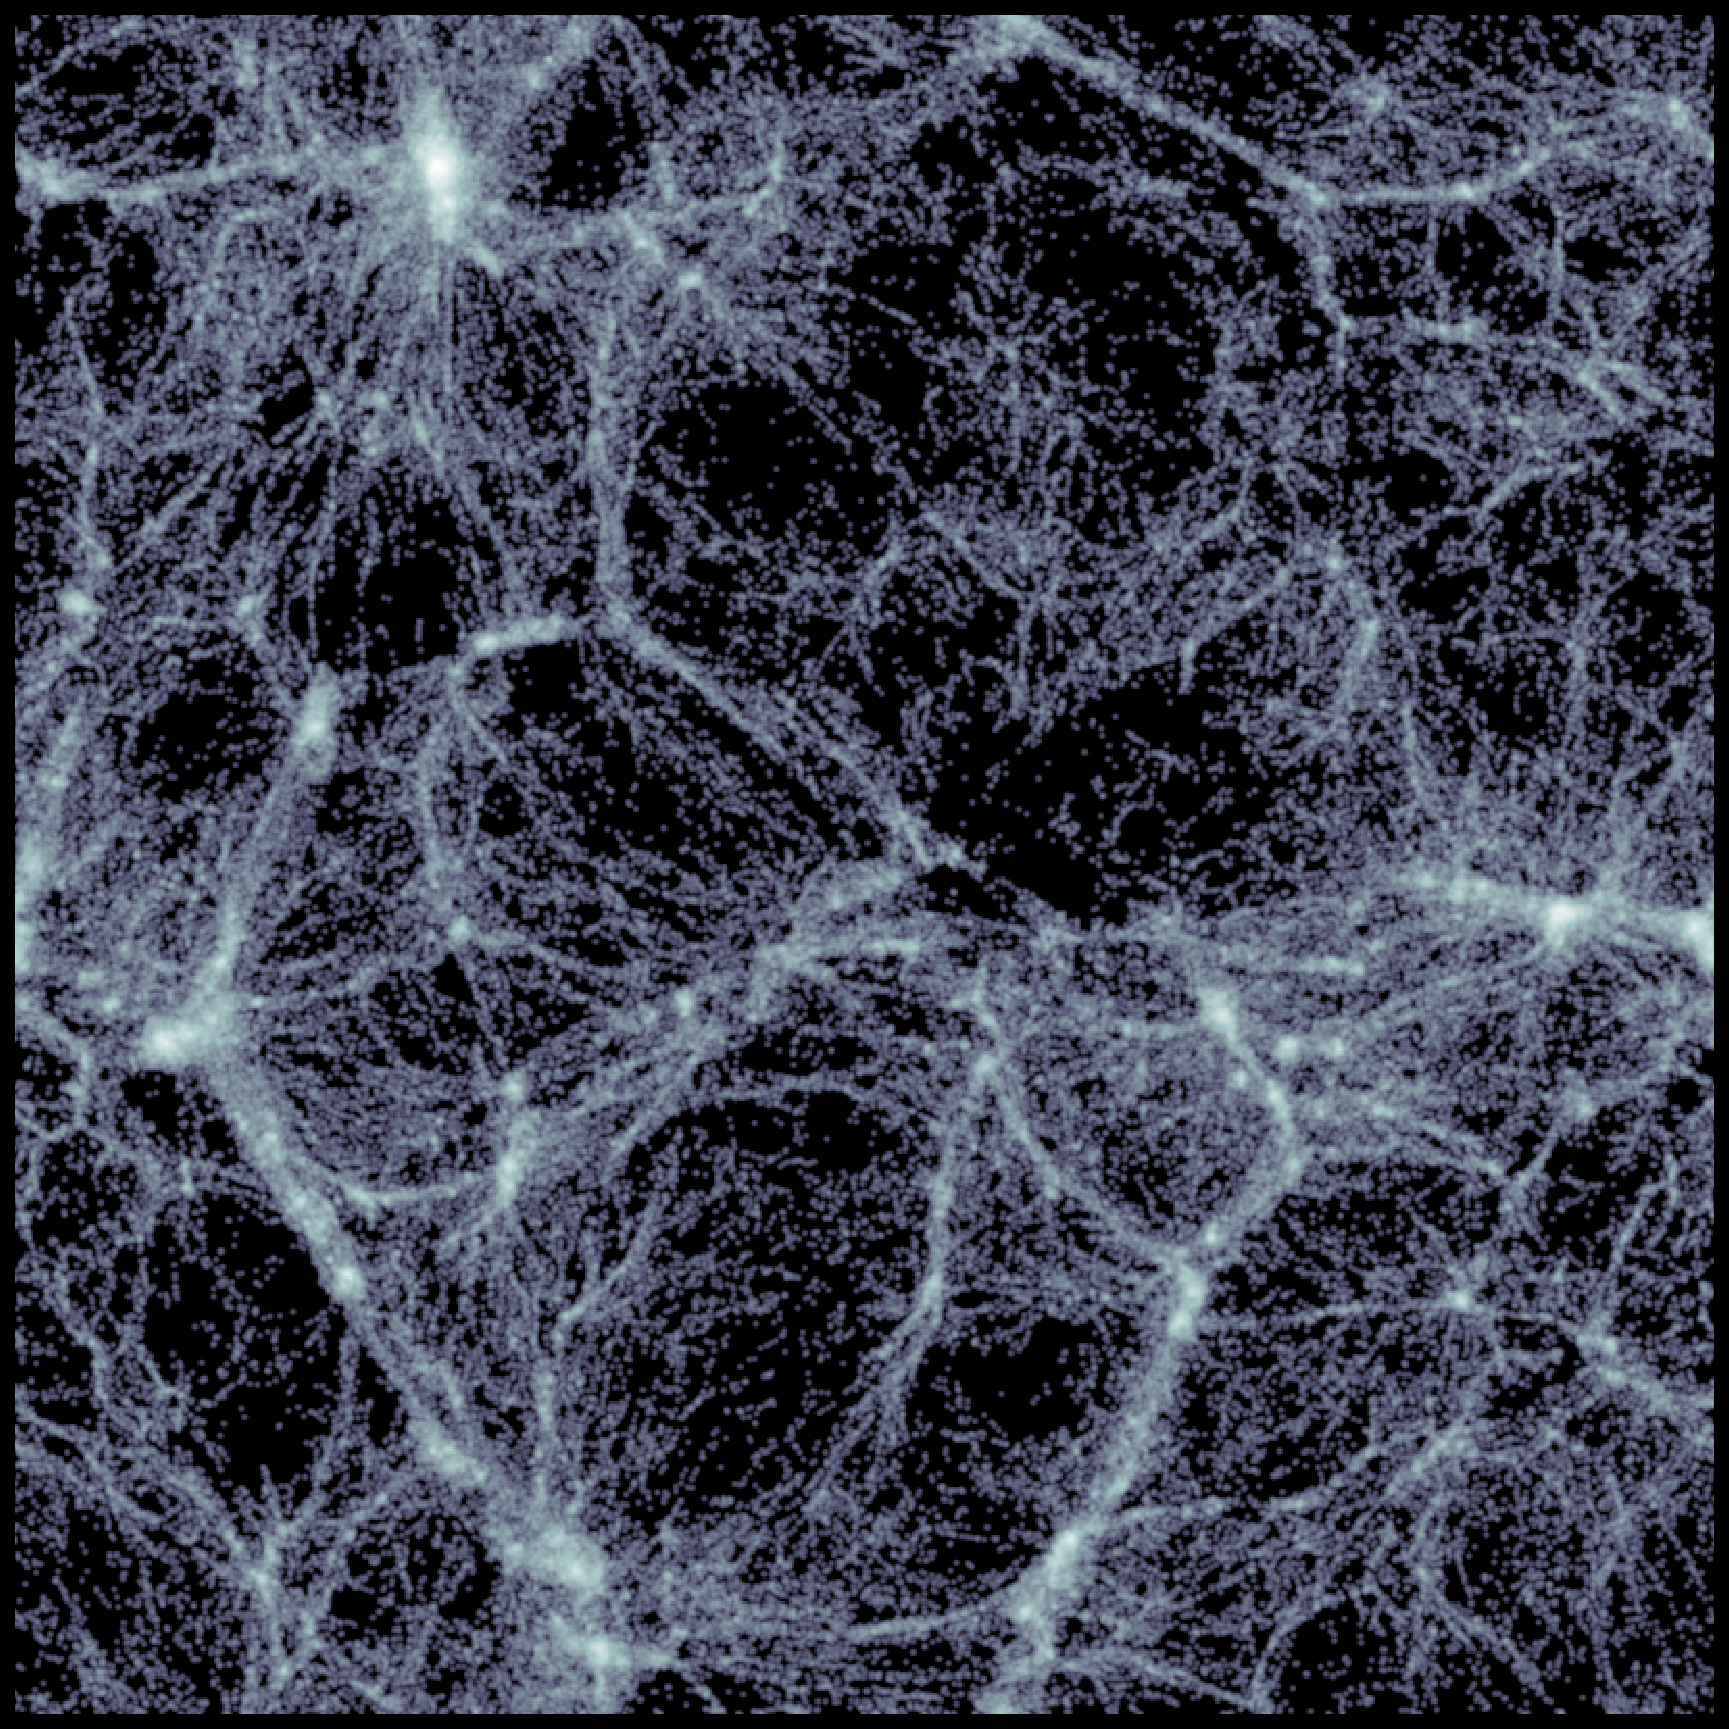
\includegraphics[width=\linewidth]{thesis/latex/intro_files/slice_image_bone.pdf}
    \caption{Distribution of galaxies in the IllustrisTNG100 simulation. Galaxies naturally trace the anisotropic nature of large scale structure formation, with large filamentary networks on multiple scales connecting the overdensities and encasing the underdensities. Colour scale goes from dark to light corresponding to low to high densities of galaxies.}
    \label{fig:cosmo_web_tng}
\end{figure}

As the baryonic gas flows within the gravitational potential well imposed by the web-like distribution of dark matter, material is advected giving rise to a fundamental connection between large scale structure and angular momentum in galaxies. Extending the formalism of TTT to include large scale structure formation \citep[e.g.][]{pichon2011, codis2015, laigle2015}, the angular momentum distribution of galaxies can be described relative to their neighbouring walls and filaments. In cosmological simulations, this can be seen as a mass dependent alignment between the spin of the dark matter haloes and the filament direction. The spin vectors of low mass haloes orient along the filament indicative of advection of angular momentum from the filament itself. Conversely high mass haloes have undergone mergers in the plane of the filament leading to a `flip' in orientation. How the spin of the haloes propogates to that of the baryonic components is complex and hence observations of this effect are inconclusive \citep[e.g.][]{tempel2013, krolewski2019, welker2020}. 

\section{Halo assembly bias}
As introduced in \S\ref{sec:ang_mom_intro}, bottom-up assembly in $\Lambda$CDM of dark matter haloes can be explained approximately by the excursion-set formalism which tracks the linear growth of primordial over-densities before spherically collapsing in the non-linear regime \citep{press1974,bond1991}. In the most basic form, environment is neglected and the assembly history of the halo is entirely dictated by its mass. This exclusive dependence on mass underlines the widely used halo occupation distribution \citep[HOD; e.g.][]{jing1998,peacock2000} modelling and various types of abundance matching \citep[e.g.][]{kravtsov2004,conroy2006}, which require galaxy clustering to be driven solely by halo mass \citep[e.g.][]{mo1996,sheth1999}. 

Parallel to the successes of HOD modelling, N-body simulations have fast converged on the fact that, at fixed halo mass, haloes which have formed at different times cluster differently \citep[e.g.][]{gao2005,wechsler2006,croton2007,wang2011}. Termed \textit{halo assembly bias}, this quantifies any physical quantity of a dark matter halo which correlates with halo clustering beyond the driving factor of halo mass. While most commonly considered as halo formation time, properties such as halo spin and concentration have also been demonstrated to be related with clustering \citep[e.g.][]{lacerna2012,lehmann2017}. 

Attempts to understand the origin of assembly bias have come from the large-scale tidal environment in which the given halo resides. Large-scale tidal forces are naturally anisotropic and intimately connected with the structure of the cosmic web. Halo assembly can therefore be de-convoluted as the influence of small and large scale forces. On small scales, gravity is dominant and the key properties are driven by local overdensity, encoded by the total mass of the halo. On large scales, the impact is more subtle \red{nuanced?}.

In simulations, \citet{hahn2009} found a systematic trend between halo formation time and the large-scale tidal force strength, derived from the geometric environment, at fixed halo mass. This effect is seen most strongly in low-mass haloes, arising from suppression of their growth when they reside within the vicinity of a much larger halo. This large halo acts to stop accretion on the low-mass halo in over-dense regions, effectively boosting the clustering of older low-mass haloes, compared to haloes of the same mass residing in under-dense regions that are less affected by tidal fields. \citet{ZOMGI} explore this phenomenon in the context of the cosmic web. Low-mass haloes residing within large filaments can often see their accretion `stalled' and hence will cease mass assembly earlier as matter flows preferentially along the filament to its densest points (nodes). Conversely low-mass haloes at the convergence point of multiple smaller filaments will have continued isotropic accretion resulting in longer continued mass growth and more recent formation. \citep[See][for a theoretical approach]{musso2018}.

Galaxies are our primary resource in probing the spatial distribution of dark matter. Their formation and subsequent evolution is tied to the assembly history of their host halo, however, determining the exact link is difficult. The observational counterpart of assembly bias is therefore tricky to isolate and as such is rightfully still under debate. In the context of galaxy evolution, the question of halo assembly bias can be rephrased to; \textit{does the cosmic web significantly impact galaxy evolution once stellar (or halo) mass has been accounted for?}

Early studies, however, have demonstrated observations of halo assembly bias. For example, \citet{tojeiro2017} compare a halo age proxy with respect to large-scale tidal environment defined in the Galaxy And Mass Assembly \citep[GAMA;][]{driver2009, driver2011} survey. They quantify tidal strength using the geometric classification of \citet{eardley2015} to characterise regions into geometric voids, sheets, filaments and knots corresponding to zero, one, two and three dimensions of collapse respectively. They find that low-mass haloes ($\lesssim 10^{12.5} M_{\odot}$) show a steadily increasing ratio of central galaxy stellar mass to total halo mass, corresponding to increasing halo age in regions of increasing tidal force strength (i.e. going from voids to knots). They find a tentative reversal of this trend for high-mass haloes ($\gtrsim 10^{13.2} M_{\odot}$). \citep[See][who explicitly look for changes in halo to stellar mass ratio with geometric environment using stacked lensing profiles, but find no significant changes when averaging over halo mass.]{brouwer2016}.

The tidal field can also be described in a topological sense with respect to the cosmic web. \citet{kraljic2018} provide an investigation in the GAMA survey through identification of the cosmic web, using the Discrete Persistent Structure Extractor code \citep[DisPerSE;][]{sousbie2011a,sousbie2011b}. \red{introduce disperse here?} They estimate distances to nodes, filaments and walls as a function of galaxy properties such as $u - r$ colour, specific star formation rate (sSFR) and stellar mass. They find distinct gradients with more massive, redder (passive) galaxies residing closer to nodes, filaments and walls, indicative of mass dependent clustering. Additionally, at fixed stellar mass, both star formation rate (SFR) decreases and colour reddens for galaxies closer to both nodes and filaments. Assuming the flow of baryonic accretion follows that of dark matter, this observation is consistent with the `stalling' of haloes due to tidal environment.

\section{This thesis}
In this thesis, I want to help answer three questions:

\begin{itemize}
    
    \item Why does the rotation of ionized gas decouple from the overall rotation of a galaxy, and how is this related to the angular momentum content of the dark matter halo?
    
    \item Are signatures of halo assembly bias detectable in galaxy observables such as kinematic misalignment or galaxy spin? \red{maybe rephrase this question?}
    
    \item How does the anisotropy of the cosmic web impact both the kinematics within galaxies and the dynamics of galaxies in the larger potential well of the overall halo?
    
\end{itemize}

In Chapter 2, I introduce the concept of kinematic misalignment and how this can be utilized in large scale Integral Field Spectroscopic surveys. In Chapter 3, I use an observational sample of misaligned galaxies to understand their typical characteristics and fundamental relationships with other observable properties. In Chapter 4, I introduce a mock observational sample created from a cosmological scale hydrodynamical simulation to understand if the observational trends can be reproduced and what can be learned from their evolutionary histories. In Chapter 5, I investigate the relationship between black hole activity in this mock sample and the relationship with kinematic misalignment. In Chapter 6, I investigate if kinematic misalignment in observations can be related to various measures of the assembly history of the surrounding dark matter halo. In Chapter 7, I investigate the differences between the orbits of satellite galaxies in different environments of the cosmic web and the potential for this to be recovered by dynamical models. In Chapter 8, I present results relating the spin alignment of galaxies with large scale structure in a large scale Integral Field Spectroscopic survey. In Chapter 9, I relate the angular momentum content of galaxies and dark matter haloes to the initial conditions of a hydrodynamical simulation.
\colorlet{chaptergrey}{black!10!yellow!20!green!35!}
%\renewcommand*\sectfont{\color{orange}}

\chapter[Kinematic misalignment]{Kinematic misalignment in observations and simulations}
\label{ch:kin_mis}
\vspace{-5.25in}
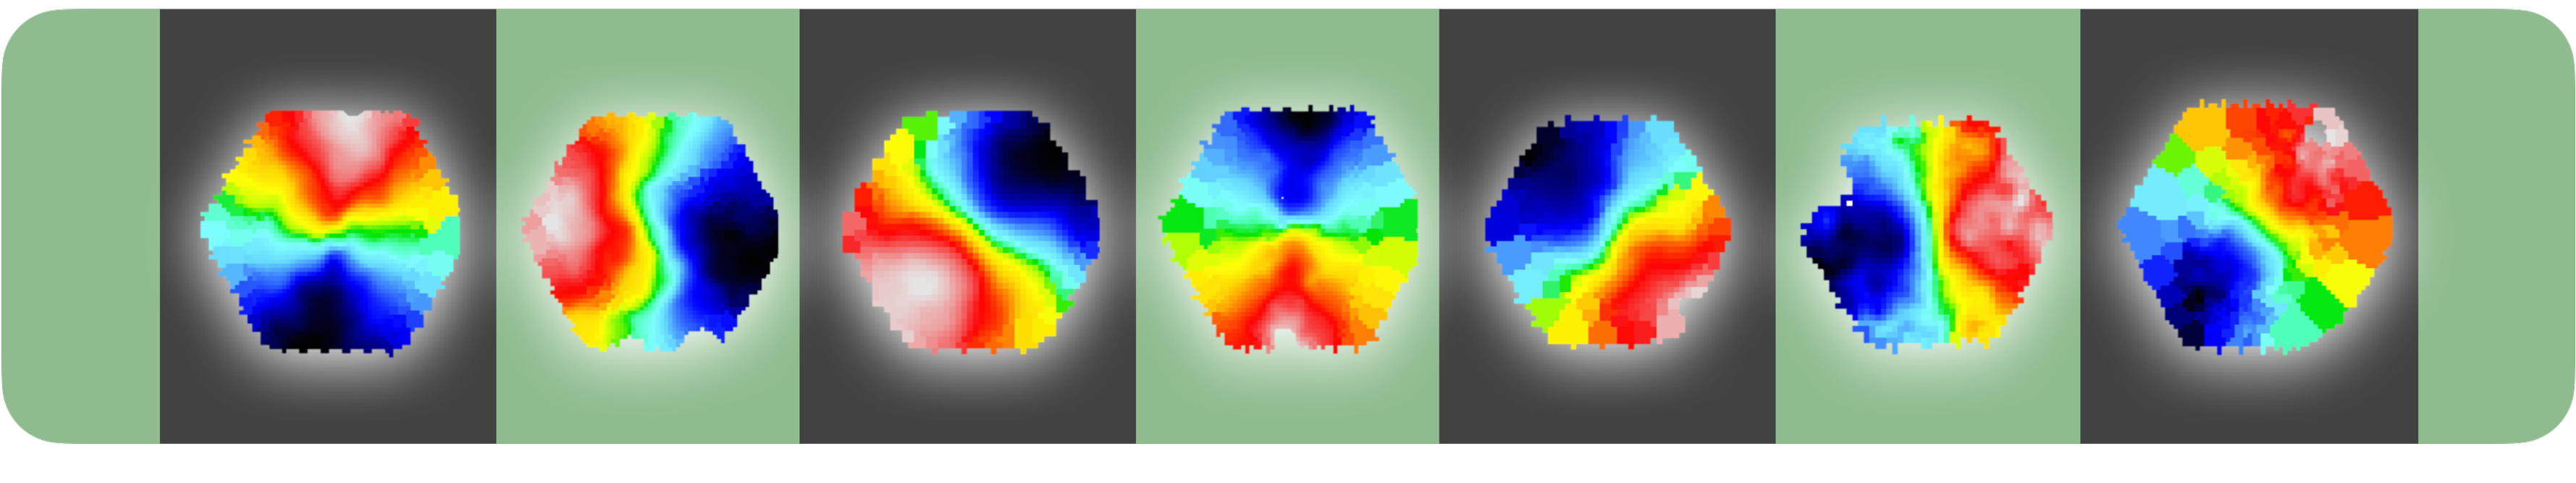
\includegraphics[height=1.33in]{thesis/latex/headers/green_ifu.pdf}
\vspace{3in}

\epigraph{This chapter is predominately based on Duckworth, Tojeiro and Kraljic, in MNRAS 492, Issue 2, 2020, however also is also partially based on sections of Duckworth, Tojeiro, Kraljic, Sgr\'o, Wild, Weijmans, Lacerna and Drory, in MNRAS, 448, Issue 1, 2019. Here, we introduce kinematic misalignment and investigate the relationship of kinematically misaligned galaxies with morphology, angular momentum, and, gas content in both observations and simulations.} 

\section{Introduction}
%Studies in more recent IFS surveys and simulations have demonstrated the close interlink between stellar angular momentum, stellar mass and morphology suggesting that late types and early type fast rotators form a continuous sequence rather than from fundamentally different formation pathways \citep[][]{cortese2016, lagos2017, graham2018}. Remarkably, despite the highly non-linear processes involved, current cosmological surveys predict that the stellar angular momentum in rotationally supported galaxies at $z=0$ is still conserved from that of the dark matter halo \citep[e.g.][]{genel2015}. 
While the stellar continuum is often considered for studies of angular momentum, optical integral field spectroscopic (IFS) observations also provide kinematic information of the ionized gas in the galaxy. In the basic picture of tidal tensor theory, stars form from the collapsing gas, leading to the expectation that they inherit its dynamics and hence galaxies have coherent rotation between their stars and gas. Unsurprisingly galaxy evolution is complex and galaxies seldom form in isolation, resulting in a significant proportion of galaxies with decoupled rotation between their stars and ionized gas. 

An offset between the rotation of stars and ionized gas has been motivated to be of external origin \citep[see;][]{sarzi2006,davis2011}. The ability of a given galaxy to accrete cold gas determines its continued ability to form stars, and hence, dictates where it falls amongst the Hubble sequence. Accreted gas has many origins (such as filamentary `cold mode' accretion from the cosmic web, mergers or additionally cooling flows from a shocked hot halo), however, is converted into stars within typical depletion timescales of order gigayears \citep{davis2016}. 
For material stripped in mergers, or for shocked gas accreting through cooling flows, a natural consideration is that the accretion may not be necessarily aligned with the angular momentum of the benefiting galaxy \citep[e.g.][]{davis2011, lagos2015}. Misalignment can be considered to be a transient property as torques from the stellar component continually act to realign the gas component which can only be opposed by sustained misaligned accretion \citep[][]{vdvoort2015, davis2016}. 

Understanding the origin, nature, and, prevalence of galaxies with decoupled star-gas rotation (i.e. kinematic misalignment - used interchangeably) has been the focus for several recent works. \citet{davis2011} found that $\sim 36$\% of ETGs exhibit misalignment between their star and gas rotation (i.e. a difference of at least 30$^{\circ}$ between rotational axes) within the volume-limited sample of ATLAS\textsuperscript{3D} \citep{atlas3d}. This fraction increases when considering field (isolated) ETGs, giving a first suggestion at an environmental dependence. For late types, \citet{chen2016} first investigated star forming galaxies with counter-rotating stars and gas (i.e. a difference of at least 150$^{\circ}$ between rotational axes), a far rarer occurrence ($\sim$2\%), finding a clear boost in star formation in central regions. This could suggest that the processes leading to significant misalignment are also inherent in cancelling angular momentum, enabling increased gas in-flows to nuclear regions. \citet{jin2016} extended this discussion to find that for a sample of 66 misaligned galaxies, the misalignment fraction ($> 30^{\circ}$) is dependent on properties such as specific star formation rate, stellar mass and local environment, again determining that misaligned galaxies are more isolated. 

Despite this, kinematic misalignment appears to be correlated with mergers and interactions. In CALIFA, \citet[][]{barrera2015} investigated a range of interacting galaxies (i.e. at different stages of a merger) in comparison to a non-interacting control. They demonstrate that interacting galaxies of all stages demonstrate both more significant misalignment between stars and gas (represented by global position angles; i.e. PA for the total velocity field), but also that position angles are more likely to deviate as a function of radius for any given component. This is corroborated by \citet{li_decoupling2019} who investigated the relationship between kinematic misalignment in MaNGA and deeper photometry in the Dark Energy Spectroscopic Instrument (DESI) Legacy Imaging Surveys \citep{dey2019}. They find that up-to 40\% of misaligned galaxies in MaNGA can be attributed to ongoing or recent mergers/interactions, underlining the importance of external processes. 

This likely represents a lower limit on the importance of interactions due to the typical timescales of misalignment. \citet{davis2016} utilise a toy model to propose that misaligned gas could relax gradually over time-scales of 1-5 Gyr. A faster time-scale of relaxation would require merger rates of $\approx 5$ Gyr\textsuperscript{-1} and hence is disfavoured. The interplay between the strength and persistence of the gas in-flow and the re-aligning torque of the stellar component dictates the exact time-scale of misalignment for an individual galaxy. The strength of a galaxy's stellar torque scales as a function of radius, with the central component of a galaxy re-aligning on a quicker time-scale than the outer regions. The persistence of misalignment has also been considered in numerical simulations. \citet{vdvoort2015} consider the evolution of a misaligned gas disk formed from a merger which removes most of the original disk. During re-accretion of the cold gas, the misaligned disk persists for approximately 2 Gyr before the gas-star rotation angle falls below 20$^{\circ}$. The sustainment of this misalignment is due to continued gas accretion for approximately 1.5 Gyr before its rate falls and the gas can realign with the stellar component on approximately six dynamical time-scales. 

In the field of kinematic misalignment, direct comparison between observations and simulations have been made in parallel during the time of this thesis work. In the SAMI survey, \citet{bryant2019} utilised misalignments for $\sim$1200 galaxies, demonstrating that morphology holds the strongest correlation with the likelihood of star-gas decoupling, ahead of local environment and stellar mass. A direct comparison of this observational SAMI sample to the cosmological simulation of \texttt{Horizon-AGN} is made by \citet{khim2019}. They find that a selected subsample of galaxies in \texttt{Horizon-AGN} reproduces the general trends of misalignment fraction with morphology and stellar mass. Despite this, they find that simulated galaxies in clusters are far more likely to be misaligned than their observed counterparts. Finally, there is observational evidence \citep[e.g.][]{davis2016, chen2016} that counter-rotation between stars and gas (usually defined as $> 150^{\circ}$) is a stable-state leading to a boost in galaxies with these typical offsets. This isn't reproduced by \texttt{Horizon-AGN}, likely due to the spatial resolution of the simulation (roughly 1kpc) which is difficult to resolve thin disks and hence realistically balance the effect of stellar torques and relaxation. A caveat in the work of \citet{khim2019} is that they do not aim to directly recreate the SAMI sample or mock observations, which convolutes physical differences between observation and simulation with discrepancies due to measurement and how properties are computed. 

Finally, \citet{starkenburg+19} considered the nature of counter-rotation ($\mathrm{> 90^{\circ}}$ between rotational axes of stars and gas) in low mass galaxies in the \texttt{Illustris} simulation \citep{vogelsberger2014a, vogelsberger2014b, genel2014, sijacki2015}. They identify the key role of gas loss through black hole (BH) feedback and flyby interactions to enable misalignment through re-accretion of misaligned material. The mechanisms for decoupling gas are not fully determined and are likely a combination of both external and internal processes, both of which are seen to also shape the stellar angular momentum content of galaxies at $z=0$. To understand how these non-linear processes relate both to angular momentum retention from the dark matter halo and how this propagates to star-gas decoupling, a combination of both observations and simulations are required. 

In this Chapter, we investigate kinematic misalignment in the MaNGA IFS survey (\S\ref{sec:manga_kin_mis}), and make direct comparison to the hydrodynamical simulation of \texttt{IllustrisTNG} (\S\ref{sec:tng_kin_mis}). Specific to observations; in \S\ref{sec:manga_intro} we introduce the MaNGA survey and associated data output, before describing the methodology in defining kinematic misalignment. \S\ref{sec:data_obs} gives a description of the additional data catalogues used in this work and \S\ref{sec:results_obs} describes the observational properties of misaligned galaxies, before summarising our observational findings in \S\ref{sec:summary_manga}. In the second half of the chapter, we describe the construction of a mock MaNGA sample created in \texttt{IllustrisTNG} and make direct comparisons to the observational results, before investigating the evolution histories of angular momentum. Specific to simulations; \S\ref{sec:sim_data_TNG} introduces the \texttt{IllustrisTNG} simulation and the creation of the mock observational sample. \S\ref{sec:manga_tng_comp} makes direct comparison between \texttt{IllustrisTNG} and MaNGA. \S\ref{sec:tng_ang_mom_evo} describes the evolutionary histories of angular momentum for the misaligned galaxies before summarising in \S\ref{sec:tng_summary}. We discuss the implications of the chapter in \S\ref{sec:tng_discussion}.

\section{In MaNGA} \label{sec:manga_kin_mis}
\subsection{The MaNGA survey} \label{sec:manga_intro}
Set to complete in 2020, the MaNGA survey is designed to investigate the internal structure of $\sim$10000 galaxies in the nearby Universe. By design, the complete sample is unbiased towards morphology, inclination and colour and provides a near flat distribution in stellar mass. 
MaNGA is one of three programs in the fourth generation of the Sloan Digital Sky Survey (SDSS-IV) which enables detailed kinematics through integral field unit (IFU) spectroscopy. MaNGA uses the SDSS 2.5 metre telescope in spectroscopic mode \citep{gunn2006} with the two dual-channel BOSS spectrographs \citep{smee2013} and the MaNGA IFUs \citep{drory2015}. MaNGA provides spatial resolution on kpc scales (2'' diameter fibres) while covering 3600-10300$\mathrm{\mathring{A}}$ in wavelength with a resolving power that varies from R$\sim$1400 at 4000$\mathrm{\mathring{A}}$ to R$\sim$2600 at 9000$\mathrm{\mathring{A}}$. 

MaNGA observations use SDSS style plates, where bundles of optical fibres are plugged into the plate corresponding to the position of the target galaxy in the observational field. A dithered pattern is employed for each target field (plate), which simultaneously observes galaxies through 17 fibre-bundles of 5 distinct sizes. Any incomplete data release of MaNGA should therefore be unbiased with respect to IFU sizes and hence a reasonable representation of the final sample.

The majority of observations contribute to one of the three main subsets: the Primary sample, the Secondary sample and the Colour-Enhanced supplement. All sub-samples observe galaxies to a minimum of $\sim 1.5$ effective radii ($\mathrm{R_{e}}$) with the Secondary sample increasing this minimum to $\sim 2.5 \mathrm{R_{e}}$. The Colour-Enhanced supplement fills in gaps of the colour-magnitude diagram leading to an approximately flat distribution of stellar mass for the total sample. A full description of the MaNGA observing strategy is given in \citet{law2015obs,yan2016obs}. The raw observations are processed by the MaNGA Data Reduction Pipeline (DRP) as described in \citet{law2016drp, yan2016spec}. The fibre flux and inverse variance is extracted from each exposure, which are then wavelength calibrated, flat-fielded and sky subtracted.

MaNGA releases data periodically in the form of MaNGA Product Launches (MPL), both increasing the number of observed galaxies and updating the data processing. In the following chapters we use data from MPL-6 through to MPL-9 referring to the sixth and ninth Product Launches.
% Include a figure showing the distribution of NSA, MaNGA targets, MPL-6 and MPL-8.
% Also include figure of bundle sizes?
 
\subsubsection{Velocity fields} \label{sec:vel_fields_intro}
The MaNGA Data Analysis Pipeline \citep[DAP][]{westfall2019,belfiore2019} provides science-ready processed data for MaNGA observations. Some example outputs include; spaxel-by-spaxel coordinate information based on the isophotal ellipticities from the NASA-Sloan Atlas \cite[NSA; used for target selection in MaNGA;][]{blanton2011}, S/N measurements, binned spectra, stellar kinematics and stellar-continuum models, emission-line properties and models, and spectral-index measurements. Kinematics are easily accessible as 2D maps which we use for stellar and gas velocity fields in the following analysis. A complete discussion can be found in \citet{westfall2019,belfiore2019}, however we will summarise the key points concerning the construction of stellar and gas velocity fields here.

The DAP extracts stellar kinematics using the Penalised Pixel-Fitting (pPXF) method \citep{cappellari2004,cappellari2017}. The DAP fits the stellar continuum of each spaxel to extract the line of sight velocity dispersion and then fits the absorption-line spectra from a set of 49 clusters of stellar spectra from the MILES stellar library \citep{sanchez2006,falcon2011}. Before extraction of the mean stellar velocity, the spectra are spatially Voronoi binned to $g$-band \textit{S/N} $\sim$ 10, excluding any individual spectrum with a $g$-band \textit{S/N} < 1 \citep{cappellari2003}. This approach is geared towards stellar kinematics as the spatial binning is applied to the continuum \textit{S/N}, however, we note that unbinned and Voronoi binned velocity maps produce similar results (at least for the purpose of kinematic misalignment). 

Ionized gas kinematics are extracted by the DAP through fitting a Gaussian to the H$\alpha$-6564 emission line, relative to the input redshift for the galaxy. This velocity is representative for all ionized gas, since the parameters for each Gaussian fit to each emission line are tied during the fitting process. These velocities are also binned spatially by the Voronoi bins of the stellar continuum. 

\subsubsection{Kinematic misalignment} \label{sec:kin_mis}
We estimate the two dimensional global position angle (PA) of the stellar and H$\alpha$ gas velocity fields using the \texttt{FIT\_KINEMATIC\_PA} routine outlined in Appendix C of \citet{krajnovic2006}. By default this finds the angle corresponding to the bisecting line which has greatest velocity change along it (i.e. the angle of peak rotational velocity). We choose this angle to be found from sampling at 180 equally spaced steps. This is measured counter-clockwise from the north axis, however, it does not discriminate between the blueshifted and redshifted side since it is only defined up to 180$^{\circ}$. As a result, velocity fields with a difference of 180$^{\circ}$ PA would appear to be aligned. To solve this we identify the direction of rotation and re-assign a consistent PA: defined as the axis of rotation approximately 90$^{\circ}$ clockwise from the blueshifted side. This angle now spans 360$^{\circ}$ allowing an automatic detection of misaligned gas and stellar components. The offset angle between kinematic components is defined as: 
\begin{equation} \label{eq:delPA}
\mathrm{\Delta PA = |PA_{stellar} - PA_{H\alpha}|. }
\end{equation}
We define galaxies with $\Delta$PA > 30$^{\circ}$ to be significantly kinematically misaligned. An example of an aligned and a misaligned galaxy is shown in Figure \ref{fig:cutout_wIFU}. 

\begin{figure*}
    \centering
	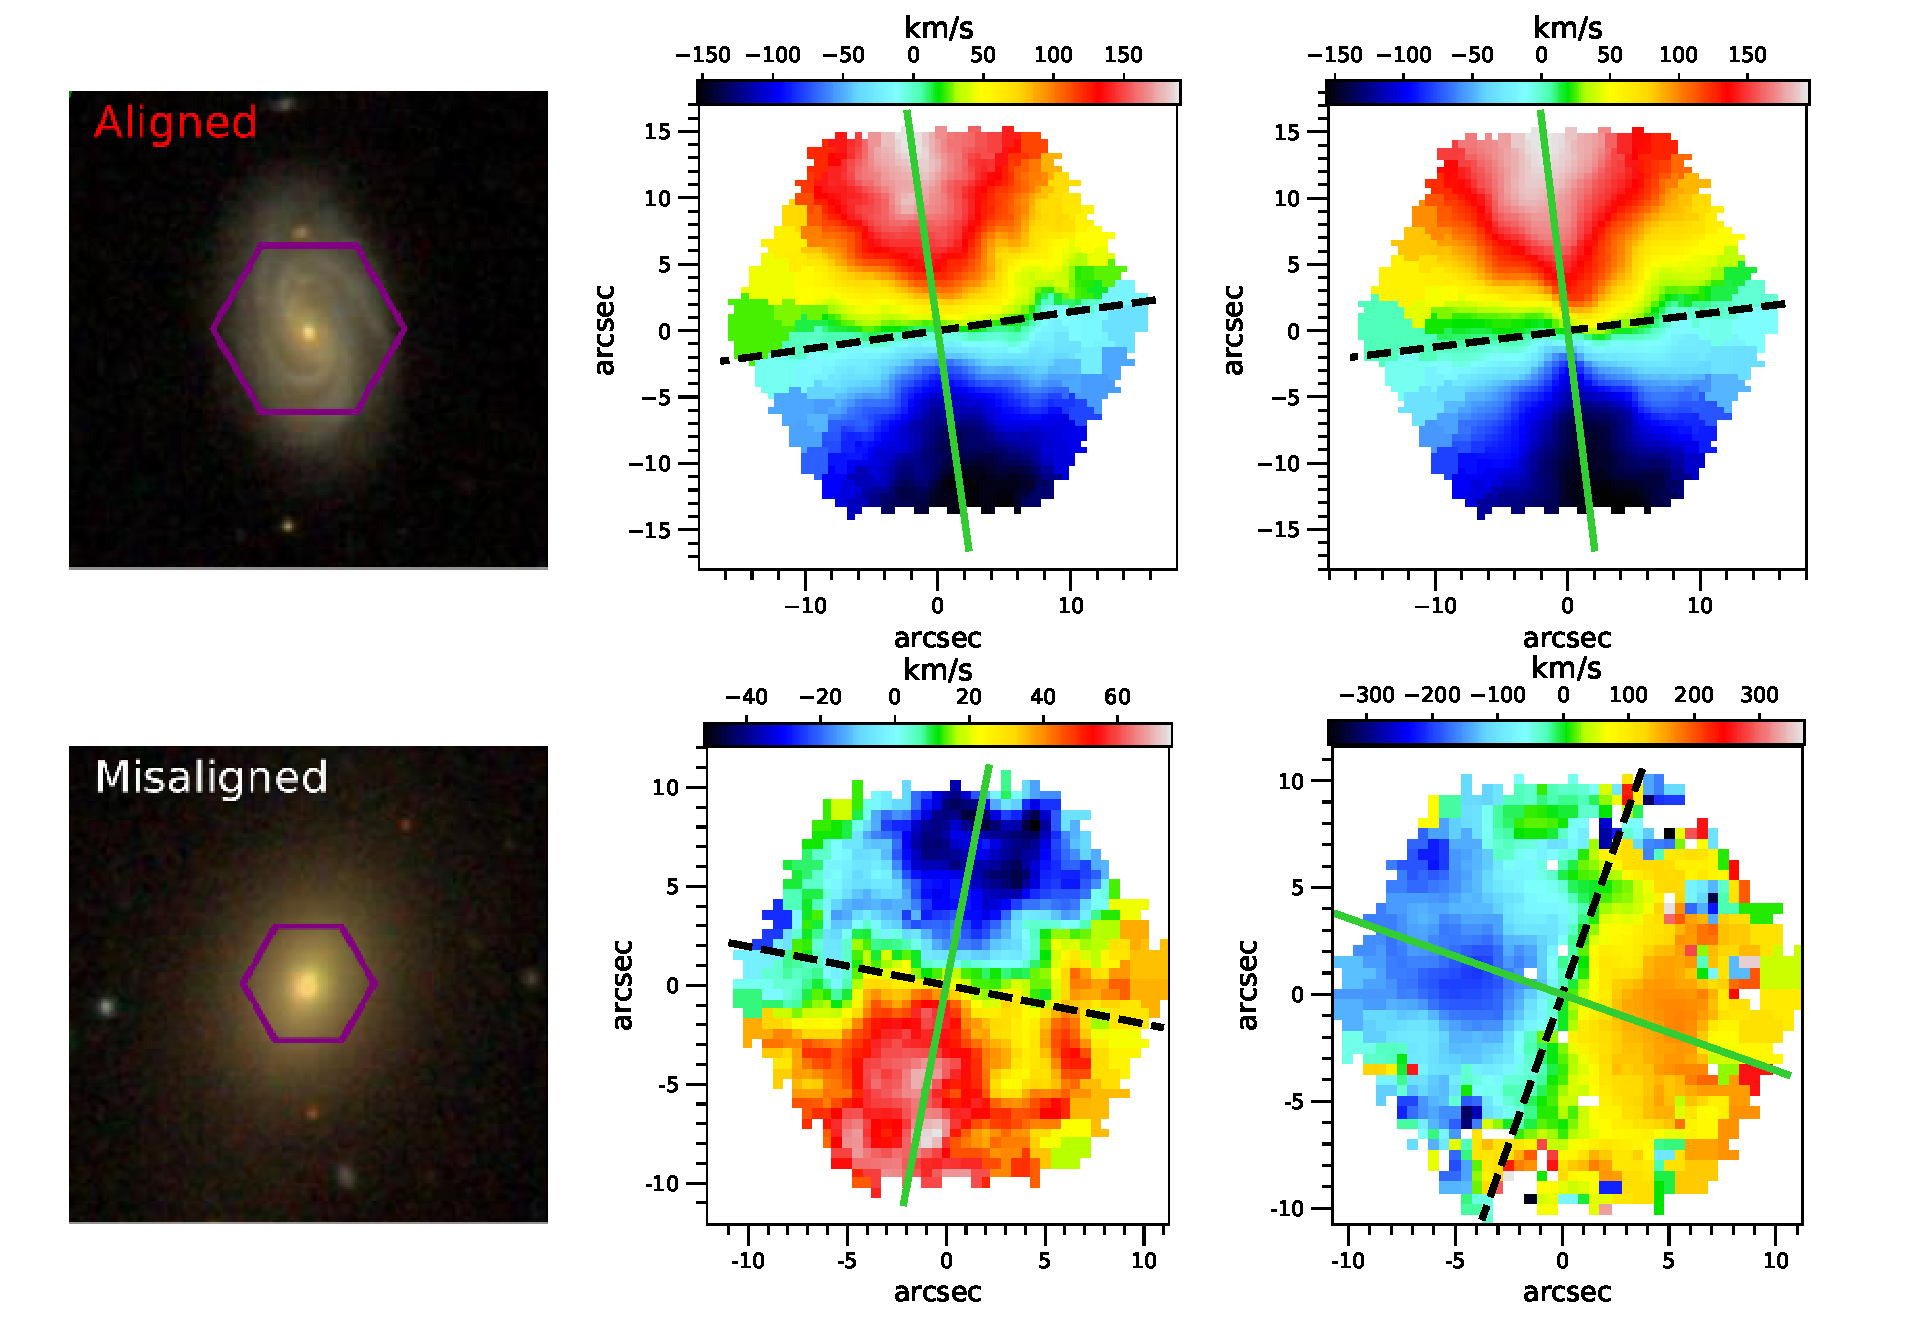
\includegraphics[width=0.8\linewidth]{thesis/latex/misalignment_MaNGA/cutout_wIFU_revised.pdf}
    \caption[Examples of a kinematically aligned (top) and misaligned (bottom) galaxy defined by $\Delta$PA.]{Examples of a kinematically aligned (top) and misaligned (bottom) galaxy defined by $\Delta$PA. From left to right, the panels show (i) the original SDSS cutout of surrounding field with the MaNGA IFU footprint overlaid in purple, (ii) stellar velocity field and (iii) $\mathrm{H\alpha}$ (gas) velocity field. The velocity fields are marked by a defined PA (green solid line) and axis of rotation (black dashed line). The galaxy in the bottom row is misaligned due to it having $\Delta$PA > 30$^{\circ}$. The colour-bars represent the velocity fields in km/s and the galaxies are orientated so that up corresponds to North and right to East.}
    \label{fig:cutout_wIFU}
\end{figure*}

To improve the reliability of the PA fit, we apply a few additional filters to the velocity fields. While foreground stars are flagged within observations, background/small neighbouring galaxies can remain within the IFU footprint. This is a problem for fitting a global position angle since it naturally interprets other material as part of the target galaxy's observation and interpolates between the regions. We remove all disconnected regions smaller than $10\%$ of the target galaxy's footprint. In addition we sigma clip the velocity field and remove all spectral pixels (spaxels) above a $3\sigma$ threshold.

Our choice to take $\Delta$PA > 30$^{\circ}$ as significantly kinematically misaligned is a conservative selection to ensure we are selecting galaxies undergoing external interaction. There is evidence to suggest that accretion drives misalignment past $\Delta$PA = 30$^{\circ}$. \citet{lagos2015} found that using solely galaxy mergers as the source for misaligned cold gas only predicts 2\% of ETGs to have $\Delta$PA > 30$^{\circ}$ using the semi analytic prescription of \texttt{GALFORM} \citep{galform}, in comparison with the misaligned field ETG fraction found in ATLAS\textsuperscript{3D} of 42 $\pm$ 6\% \citep{davis2011}. This puts a lower level of importance on gas accretion. Our choice can be justified as follows. Firstly, we are using ionized gas as a proxy for the distribution and accretion of cold gas. \citet{davis2011} find that the typical difference between the PAs of cold gas (CO) and ionized gas can be described by a Gaussian distribution centred on 0 with a standard deviation of 15$^{\circ}$ for 38 CO bright galaxies in ATLAS\textsuperscript{3D}. While indicating ionized gas is a reasonable estimator for cold gas, splitting at $\Delta$PA = 30$^{\circ}$ accounts for the scatter in this relationship. Secondly, this should avoid spurious misalignments arising from errors in the fit of $\Delta$PA. While our model errors are low (as demonstrated in the next section), they are likely an underestimation since they do not include more complex motions. However, selecting a lower split in $\Delta$PA would only be affected by the increased likelihood of internal processes being dominant, rather than the inaccuracy of fitting. Any threshold in $\Delta$PA becomes a trade off between sample size and contamination probability. Altering our cut in $\Delta$PA to be 20$^{\circ}$, 40$^{\circ}$ or similar does not change any of the conclusions drawn in this chapter.

\subsubsection{Error estimation}
It is an important point to constrain the errors of our PA fits, so we can reliably trust cuts in $\Delta$PA to select galaxies which are significantly kinematically misaligned, and hence, have had external interaction. Here, we construct two component model velocity maps for each stellar and gas component of every MPL-6 observation in order to estimate typical errors on $\Delta$PA from \texttt{FIT\_KINEMATIC\_PA} for the MaNGA sample. MPL-6 corresponds to a total of 4633 unique galaxy observations.

Errors using the \texttt{FIT\_KINEMATIC\_PA} routine have been previously estimated for molecular gas velocity fields in ATLAS\textsuperscript{3D} \citep{davis2011}. Model velocity fields with a known PA were constructed using an empirical galaxy rotation curve and combined with Gaussian noise matched to the signal-to-noise ratio of the data. A typical scatter of $\approx10^{\circ}$ was found due to varying inclination and angular resolution for the velocity fields.

\subsubsection{Circular velocity}
To find the typical error on $\Delta$PA for galaxies in MaNGA, we create model velocity maps for both the stellar and gas components of each MPL-6 observation. In each instance the basic construction of the model follows Section 4 of \citet{krajnovic2006}. Each velocity field comprises of a two-component Hernquist potential which provides a basic circular velocity given by,
\begin{equation}
\mathrm{V_c = \frac{\sqrt{GMr}}{r+r_0}}
\end{equation}
where $G$ is the gravitational constant, $M$ is the total mass and $r_0$ is the core radius of each component respectively \citep{hernquist1990}. We use a two-component model to include the relative strengths of both disk and bulge each with distinct effective radii, \re. We fix $r_0$ to be 5 and 15 (units: $arcsec$) and $\sqrt{GM}$ to be 850 and 1500 (units: $km s^{-1} arcsec^{1/2}) $ for the bulge and disk components respectively. These individual components are light weighted by model sersic flux profiles according to,
\begin{equation}
\mathrm{I(r) = I_0 e^{-\left(\frac{R}{R_e}\right)^{n_s}}}
\end{equation}
where $I_{0}$ is the peak flux and $n_s$ is the sersic index which is set to 1 and 4 for the disk and spheroidal components respectively. Since we do not have bulge-disk decompositions, we lack individual effective radii for both the bulge and disk components. Instead, we set the bulge and disk effective radii to be 0.5\re and 1.5\re, where \re is the effective radius estimated by an elliptical petrosian fit taken from the NSA targeting catalogue. 

\subsubsection{Calibration}
For each MaNGA galaxy a basic velocity field model is constructed using this template. The axes of the model velocity field are then scaled according to the inclination, $i$, which is estimated from the $b/a$ ratio taken from the NSA catalogue and is also used to scale the fraction of rotational velocity along the line-of-sight. The velocity field for each component, ($j=bulge,disk$), in polar coordinates $(r,\phi)$ is then described by,
\begin{equation}
\mathrm{V(r,\phi) = \frac{I_{j}(r)}{I_{tot}(r)}V_{c}(r)\cos(\phi+\theta_{j})\sin(i)}
\end{equation}
where $\theta_j$ is the input kinematic position angle. We set $\theta_{bulge} = \theta_{disk}$ for simplicity, however, we do note that galaxies with more complex orbital motions may increase the typical error. The position angle for both bulge and disk is simply taken to be the opening angle of the galaxy (direction of major axis taken from NSA catalogue). 

In order to imitate a MaNGA observation, the model velocity field is sampled at the spatial resolution of the corresponding IFU bundle and projected into the original shape of the actual observation for H$\alpha$ and stellar maps respectively. Gaussian noise is drawn for each spaxel from a normal distribution with the standard deviation taken from the errors on the actual observation. In addition, these model velocity fields are then Voronoi binned to match the original observation.

Example stellar and H$\alpha$ velocity fields generated from these models are shown in Figure \ref{fig:sim_ifu} with comparison to the actual observation. As expected, the model velocity fields frequently recreate observations well but struggle to encompass more complex motion. For this reason, our models should make a reasonable prediction on the typical $\Delta$PA errors intrinsic to MaNGA observations.

\begin{figure}
    \centering
	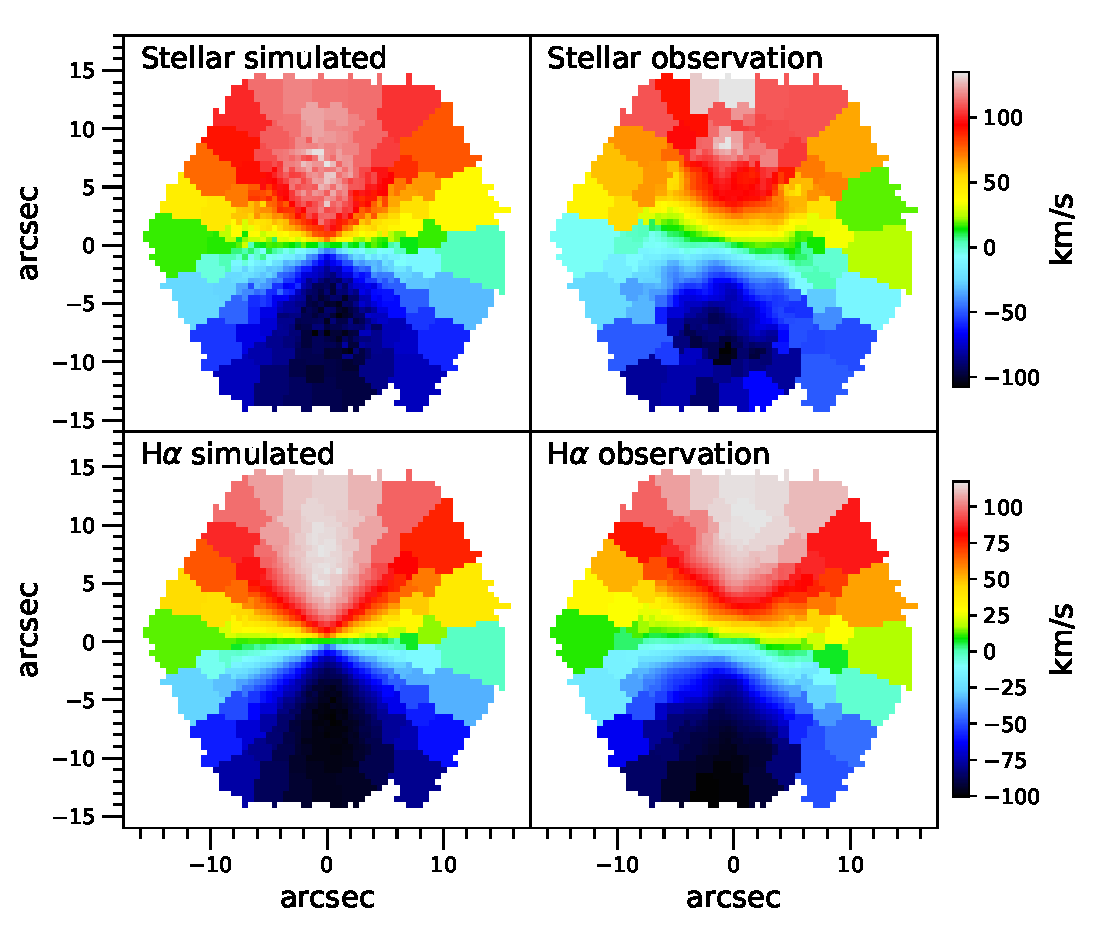
\includegraphics[width=0.7\linewidth]{thesis/latex/misalignment_MaNGA/obs_sim_IFU.pdf}
    \caption[Comparison velocity maps for a model (left column) and observation (right column).]{Comparison velocity maps for a model (left column) and observation (right column). Stellar (H$\alpha$) component velocity maps are shown on the top (bottom) row with the associated velocity colourbars.}
    \label{fig:sim_ifu}
\end{figure}

\subsubsection{Typical errors}
We construct model velocity fields for all non-critically flagged MPL-6 galaxies, inclusive of the $\Delta$PA sample used in this work. Figure \ref{fig:model_errors} shows the cumulative probability distribution for the range of $0-5^{\circ}$ where the majority of errors fall. We find that \texttt{FIT\_KINEMATIC\_PA} gives a typical combined (stellar and gas) mean error of $1.3^{\circ}$. While this is an underestimation of true $\Delta$PA errors for a sample of galaxies including those with more complex velocity fields, it is indicative that selecting a cut at $\Delta$PA = 30$^{\circ}$ should be robust to identifying galaxies with external interaction. 

\begin{figure}
    \centering
	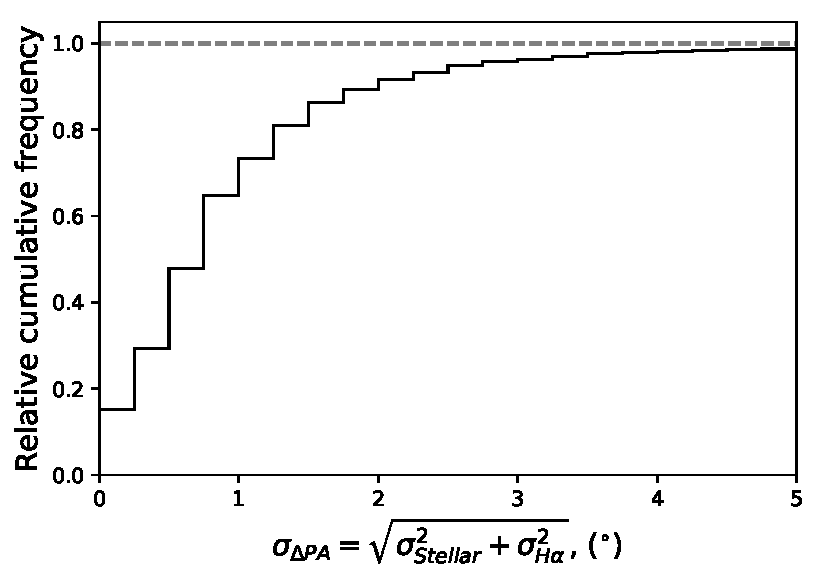
\includegraphics[width=0.6\linewidth]{thesis/latex/misalignment_MaNGA/cumulative_model_errors.pdf}
    \caption{Cumulative histogram of errors for fitting kinematic PA to model maps for the all non-critically flagged MPL-6 galaxy observations.}
    \label{fig:model_errors}
\end{figure}

\subsubsection{Visual Classification} 
Global position angles are only well defined for coherently rotating velocity fields. Those with a decoupling between inner and outer regions due to warps or kinematically decoupled cores (KDCs) are poorly described by global PAs. To select a clean sample of galaxies with well defined global PAs, we visually classify all of the velocity fields after pre-processing and PA fitting. Both stellar and H$\alpha$ velocity fields are characterised into 3 categories;
\begin{itemize}
    \item Dominant coherent rotation and well defined PA.
    \item Dominant coherent rotation but with more noise or more complex motion resulting in a usable PA fit but with higher typical errors. Highly inclined velocity fields with a higher likelihood of inaccurate PAs fits are included in this category. 
    \item Do not use.
\end{itemize}

Kinematic features are also identified. Both stellar and H$\alpha$ velocity fields are classified into;
\begin{itemize}
    \item Kinematically decoupled core (i.e. those with a central component that rotates in a different direction ($> 30^{\circ}$) with respect to the overall galaxy rotation).
    \item Warp (velocity field of central region is warped with respect to outskirts. This may be due to a bar, oval shaped structures in the disk (oval distortions) or accretion of fresh material with different angular momentum to the bulk rotation).
    \item Merger (ongoing merger or neighbour identified within IFU. Only those with obvious disruption are followed up in photometry).
    \item No features.
\end{itemize}
The majority of those with kinematic features have poorly defined global PAs and hence are flagged as do not use for the previous flag. The galaxies we refer to as `warped' represents a combination of galaxies with bars, oval distortions and differential rotation in the disk \citep[e.g.][]{barrera2014}. We direct the reader to \citet{stark2018} for an approach to separate the galaxies we refer to as warps. In this work, we enforce axisymmetry for our sample and hence make no use of galaxies that have significant variations in their PA as a function of radius.

For studies of quenching it may be useful to consider galaxies that have defined stellar rotation but lack coherent motion in the ionized gas. For galaxies that have usable PAs for the stellar velocity but unusable PAs for the ionized gas, we define a further classification of the gas velocity field;
\begin{itemize}
    \item Depletion (seen as empty spaxels signifying lack of gas, usually in central regions)
    \item No clear rotation (map has no clear rotation or is noise dominated)
    \item Partial rotation (partial coherent rotation in the velocity field, however there are significant regions with incoherent motion or noise domination)
    \item No clear characteristics/ No gas.
\end{itemize}
We note there is a clear overlap between the classifications for depletion and no clear rotation, since velocity fields are often a combination of these two features. 
%The total numbers for each classification in each category are summarised in Table \ref{tab:kin_class}. 
Examples of PA fits with the associated photometry for various kinematic classifications is given in Figure \ref{fig:mis_grid}. Examples of galaxies that are kinematically aligned, misaligned, have a stellar kinematically decoupled core, have a warped H$\alpha$ velocity field and have clear stellar rotation but depleted ionized gas/ no rotation are shown respectively.

\begin{figure*}
    \centering
	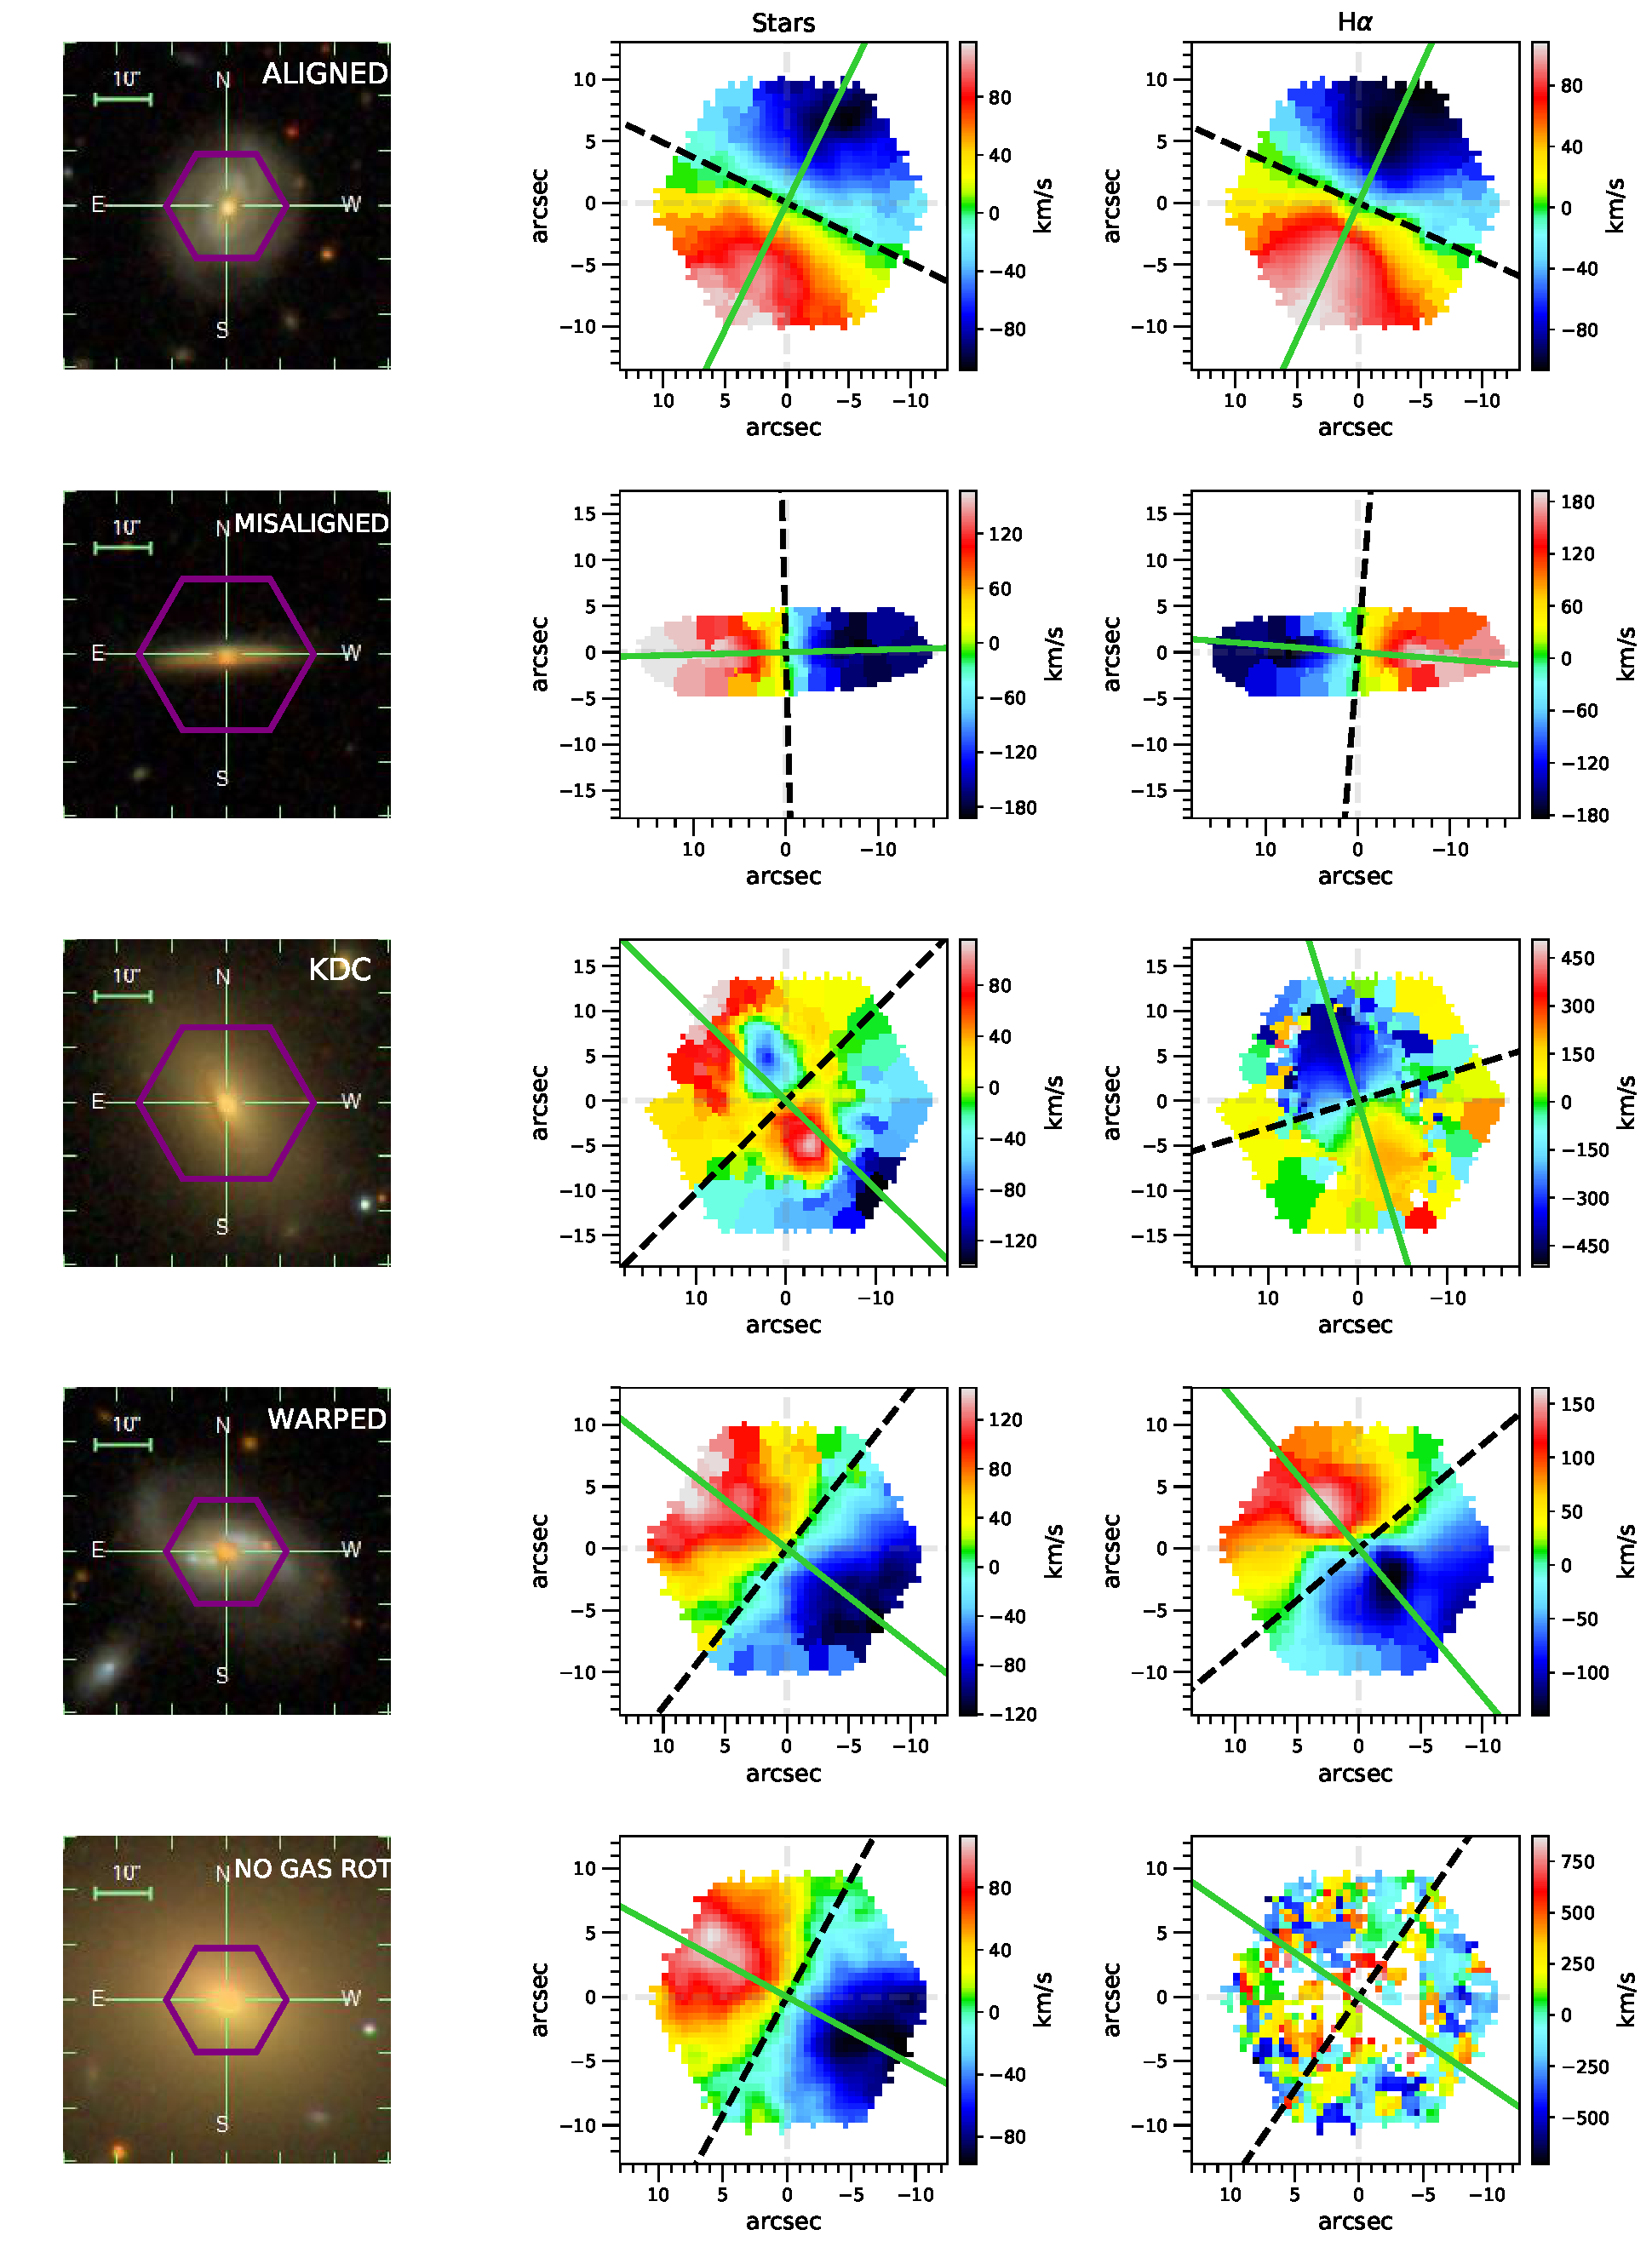
\includegraphics[width=0.93\linewidth]{thesis/latex/misalignment_MaNGA/misalignment_grid.pdf}
    \caption{Examples of PA fits for galaxies with different kinematic classifications. For each galaxy (row), we show the photometry taken from SDSS with the MaNGA IFU observation footprint overlaid in purple (left), the stellar velocity field (middle) and the H$\alpha$ velocity field (right). The kinematic PA fits (see \S\ref{sec:kin_mis}) are shown on the velocity fields (green solid line) with the axis of rotation (black dotted line). The kinematic classifications from top to bottom are; (a) PLATEIFU: 7958-6101, kinematically aligned near face on; (b) PLATEIFU: 8465-12704, counter-rotating near edge on; (c) PLATEIFU: 9868-12704, with a KDC in the stellar velocity; (d) PLATEIFU: 8252-6103, with a warped H$\alpha$ velocity field with respect to the stellar; (e) PLATEIFU: 10219-6102, with a centrally depleted/missing H$\alpha$ velocity field but coherent rotation in the stellar.}
    \label{fig:mis_grid}
\end{figure*}

\subsection{Data} \label{sec:data_obs}
This section describes the catalogues crossed matched with the MaNGA sample to seperate galaxies based on optical morphology and group membership.

\subsubsection{Morphology} \label{sec:morph_def_obs}
We classify the morphology of MaNGA galaxies through the formalism laid out by the citizen science project; GalaxyZoo2 \citep[GZ2;][]{willett2013}. GZ2 provides visually identified morphologies (and also measures finer morphological features e.g. bars, bulge size and edge-on disks) for 304,122 galaxies drawn from SDSS. GZ2, however, is not complete for the MaNGA sample and has been combined with an unpublished version; GalaxyZoo4 to provide a consistent set of definitions for all MaNGA targets\footnote{See \url{https://www.sdss.org/dr15/data_access/value-added-catalogs/?vac_id=manga-morphologies-from-galaxy-zoo}}. 

In a nutshell, GZ2 provides morphological classification through a decision tree of questions. Further questions are dependent on the answer to the previous to characterise a certain morphological type and identify finer features (see Figure 1 in \citet{willett2013} for this flowchart). From this, a table of vote fractions for each question combined with the total number of votes dictate a reliably sampled galaxy population with a set of desired morphological features. Votes by individuals are debiased (weighted) based on their reliability in comparison to known answers to the questions.

The first question in the decision tree 'Is the galaxy smooth and rounded with no sign of a disk?', which allows broad categorisation into ETGs and LTGs. We select galaxies with a debiased vote fraction > 0.7 for smooth to be ETGs and galaxies with a debiased vote fraction of > 0.7 for disk or features to be LTGs. Defining an exact population of lenticular galaxies (S0s) is tricky through public classifications. LTGs, however, can be separated based on the dominance of the bulge with respect to the disk in GZ2 through the question 'How prominent is the central bulge, compared with the rest of the galaxy?'. \citet{willett2013} demonstrate a strong correlation between bulge dominance as defined per this question and expert classifications of T-type \citep{nair2010}. Equation 19 of \citet{willett2013} provides a linear mapping from GZ2 bulge classification to expert defined morphological T-type. Care must be taken in using this linear mapping \citep[see discussion in][]{willett2013}, however, this should be a reasonable parameterisation to coarsly separate LTGs into earlier-type (S0 - Sa) and later-type spirals (Sb - Sd). We split our LTG population at T-type = 3, to give two morphological categories; S0-Sas and Sb-Sds in addition to pure ETGs.
% We split our LTG population at T-type = 3, to give three morphological categories along with pure ETGs. 

The estimates of gas mass used here for MaNGA are derived from the Pipe3D pipeline \citep{pipe3Da, pipe3Dvac}, which uses dust attenuation within the footprint of the IFU, which methodology is described in \citet{barrera2018}.

\subsubsection{Group membership} \label{sec:group_def}
To investigate different pathways leading to kinematic misalignment, we must separate galaxies into centrals and satellites. In this chapter, we identify groups based on an adaptive halo-based group finder of \citet{yang2005,yang2007} with improved halo mass assigning techniques \citep[see;][for details and application to SDSS]{lim2017}. A more detailed discussion of the effectiveness of the group finder of \citep{yang2007} (and hence for the similar catalogue presented here) is given in \S\ref{sec:mass_hab}. In a nutshell, the group finder uses either the stellar mass or luminosity of central galaxies in addition with the $\mathrm{n^{th}}$ brightest/most massive satellite as proxies for halo mass. Galaxies are assigned to groups through an iterative process, where halo properties such as halo size and velocity dispersion are updated until membership converges. 
% For groups that are outside of the redshift limit where groups are complete final halo masses are assigned through abundance matching. Those incomplete are assigned halo masses based on the ranking between halo mass and the proxy found at the final iteration of the group finder.
% The performance of the group finder has been tested on realistic mock catalogues, showing that the halo masses of individual haloes are consistent with the true mass with a typical scatter of $\sim$0.2 dex. This scatter is similar to the commonly used group finder of \citet{yang2007}, however extends uniformly to halo masses 0.7 dex lower. 

% For this work, we use the stellar mass based halo mass proxy for the SDSS main sample. 
\citet{lim2017} do not apply the group finder to the thin strips in the Southern Galatic Cap of SDSS main due to incomplete groups resulting from close proximity to borders. MaNGA galaxies in these strips are therefore unclassified by the group finder, resulting in 5088 matched galaxies with group membership classifications into central or satellite. 

\subsection{Results} \label{sec:results_obs}
We divide our MaNGA $\Delta$PA defined population at $\Delta$PA = 30$^{\circ}$ into aligned and misaligned. In the following, we also consider galaxies with defined stellar PAs but undefined H$\alpha$ due to central depletion or incoherent rotation/dispersion domination (no gas rotation; NGRs). Figure \ref{fig:delPA_stelM} shows the distribution of stellar mass for these three populations. We see no significant difference between the aligned and misaligned galaxies, however NGRs appear to be slightly more massive. \citet{graham2018} previously demonstrated the tight correlation between stellar angular momentum and stellar mass for MaNGA ($\sim$2300 galaxies). Since NGRs are slightly higher mass, it could be expected that they are typically less rotationally supported with respect to the $\Delta$PA defined populations. 

\begin{figure}
    \centering
	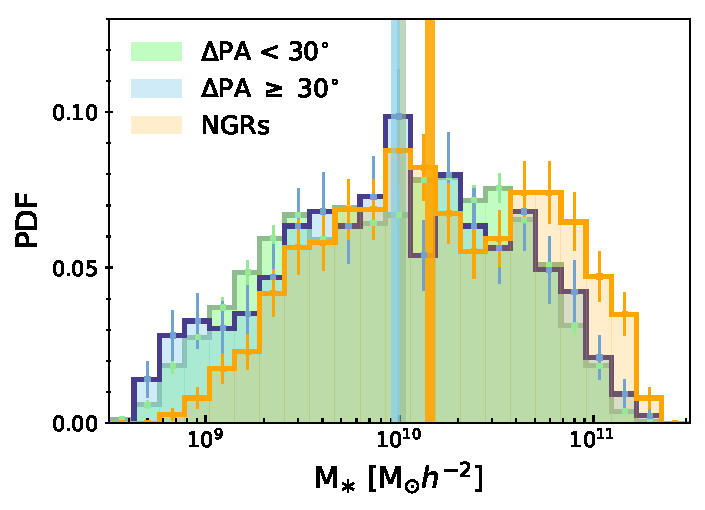
\includegraphics[width=0.7\linewidth]{thesis/latex/misalignment_MaNGA/delPA_stelM.pdf}
    \caption{Probability density distributions of stellar mass, $\mathrm{(M_{\ast}/M_{\odot})}$ for aligned galaxies ($\Delta$PA < 30$^{\circ}$) shown in green, those with high misalignment ($\Delta$PA > 30$^{\circ}$) are in blue and NGRs are in orange. Each histogram is given with Poisson errors on each bin. The vertical lines denote the corresponding distribution's median. NGRs are typically at higher stellar mass than those with aligned star and gas rotation.}
    \label{fig:delPA_stelM}
\end{figure}

Here we use the luminosity weighted stellar angular momentum estimator, $\mathrm{\lambda_R}$, taken directly from Equation 1 in \citet{emsellem2007} as
\begin{equation} \label{eq:lambda_R}
\mathrm{\lambda_{R} \equiv \frac{\langle R | V | \rangle}{ \langle R \sqrt{ V^{2} + \sigma^{2} } \rangle } = \frac{ \Sigma_{ n = 1 }^{ N } F_{ n } R_ { n } \left| V_{ n } \right| }{ \sum_{ n = 1 }^{ N } F_{n} R_{ n } \sqrt{ V_{ n }^{ 2 } + \sigma_{ n }^{ 2 } } }.}
\end{equation}
$\mathrm{\lambda_R}$ is calculated from summing over N pixels in the IFU observation within the radius of interest, $\mathrm{R}$. $\mathrm{F_{n}}$, $\mathrm{V_{n}}$ and $\mathrm{\sigma_{n}}$ are the flux, line of sight velocity and line of sight velocity dispersion of the $\mathrm{n^{th}}$ pixel. Here we present all measures of $\mathrm{\lambda_R}$ encompassing a radius of $\mathrm{1.5R_e}$ weighted by $r-$band flux. We also take the ellipticity to be $\mathrm{\epsilon} = 1 - b/a$ where $a$ and $b$ are the major and minor axes of the galaxy estimated from the NSA catalogue.

Figure \ref{fig:delPA_lambda_Re}, shows $\mathrm{\lambda_R}$ vs $\mathrm{\epsilon}$ for all $\Delta$PA defined galaxies and the medians for the aligned, misaligned and NGR samples. The black solid line overlaid shows the slow rotator regime (enclosed in bottom left). The fast/slow rotator classification refers to whether a given galaxy's rotation can be considered regular (circular velocity) or exhibits dispersion dominated motion \citep[][]{emsellem2007}. Kinematically aligned galaxies reside at preferentially higher $\mathrm{\lambda_R}$ and ellipticity with respect to NGRs. This is indicative of the dispersion dominance over rotation for disrupted gas poor and typically higher mass galaxies that we see in our NGR sample. Interestingly, kinematically misaligned galaxies also typically reside close to the slow rotator regime. In addition, the same qualitative trends are seen (i.e. misaligned and NGR galaxies have lowered angular momentum with respect to the aligned) are seen if this plot is made for ETGs, S0-Sas or Sb-Sds alone. 

\begin{figure}
    \centering
	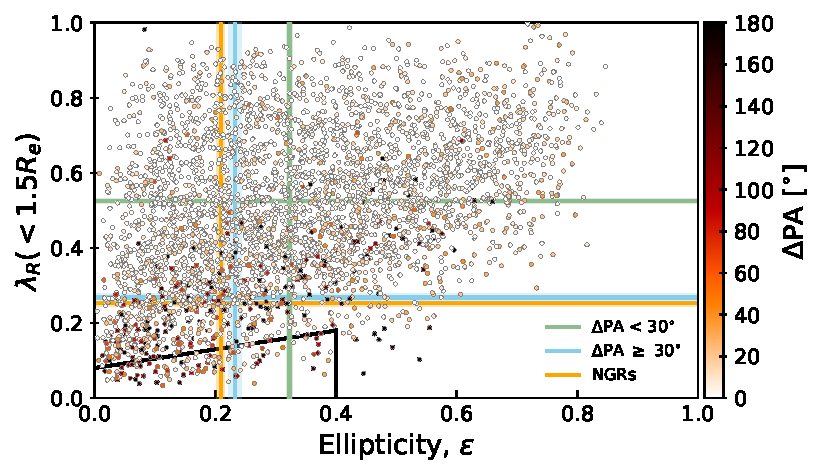
\includegraphics[width=\linewidth]{thesis/latex/misalignment_MaNGA/delPA_lambda_Re.pdf}
    \caption{$\lambda_R$ within 1.5$\mathrm{R_e}$ against ellipticity, $\epsilon$ for all galaxies with defined $\Delta$PA. The individual points are for all $\Delta$PA defined MaNGA galaxies coloured by $\Delta$PA according to the colourbar. Medians for kinematically aligned ($\Delta$PA < 30$^{\circ}$), misaligned ($\Delta$PA > 30$^{\circ}$) and NGRs are shown by the green, light blue and orange lines respectively. The lighter shade around each line corresponds to the standard error. Aligned galaxies reside more typically in the fast rotator regime with higher $\lambda_R$ and $\epsilon$, whereas misaligned galaxies and NGRs reside closer to the slow rotator regime. The same qualitative trends are found if this plot is made for ETGs, S0-Sas or Sb-Sds alone.}
    \label{fig:delPA_lambda_Re}
\end{figure}

In Figure \ref{fig:delPA_gasM} we show the distribution of gas masses for the aligned, misaligned and NGRs. We see a clear trend of lower gas mass going from kinematically aligned galaxies to misaligned galaxies to NGRs. We note that the majority ($\sim$80\%) of NGRs do not contain enough gas to have a measured gas mass from the routine of Pipe3D, so the distribution shown is a hard upper limit on the gas that these galaxies contain. We note that these trends remain qualitatively the same when considering the distributions for ETGs, S0-Sas and Sb-Sds individually.

\begin{figure}
    \centering
	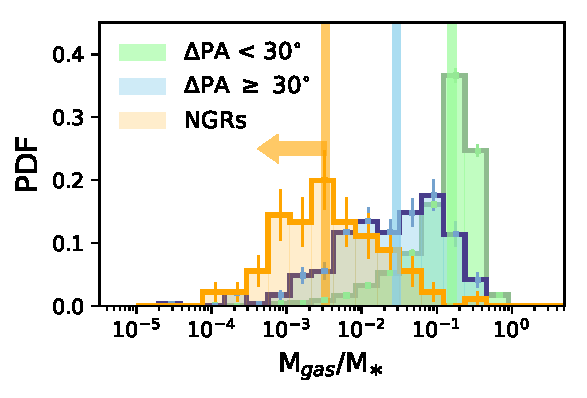
\includegraphics[width=0.8\linewidth]{misalignment_MaNGA/gas_mass_normed_all.pdf}
    \caption{Probability density distributions of gas mass fraction, $\mathrm{(M_{gas}/M_{\ast})}$ for aligned galaxies ($\Delta$PA < 30$^{\circ}$) shown in green, those with high misalignment ($\Delta$PA > 30$^{\circ}$) in light blue and NGRs in orange. Each histogram is given with Poisson errors on each bin. The vertical lines denote the corresponding distribution's median. The majority of NGRs do not have detectable gas masses and therefore the distribution shown should be considered as upper bound.}
    \label{fig:delPA_gasM}
\end{figure}

The similarity in stellar angular momentum between the NGRs and kinematically misaligned galaxies could indicate that they are from the same evolutionary sequence. A key component in decoupling star-gas rotation in simulations is a significant gas loss followed later by the accretion of material with misaligned angular momentum \citep[][]{vdvoort2015, starkenburg+19}. This gas loss can happen due to interactions from neighbouring galaxies which strips gas or through ejection due to black hole feedback.

In Chapter 5, we show that kinematic misalignment shows little relationship with distance to filamentary structure. This could point to stripped/ejected material being re-accreted as a potential source of misalignment between star and gas rotation. Some NGRs could therefore represent an earlier timestamp before this material is re-accreted. Not all NGRs would necessarily re-accrete gas, meaning that some would remain quenched (and hence would not become misaligned in the future) potentially explaining the differences we see in stellar mass distributions of NGRs and misaligned. In this scenario, it would suggest that re-accretion of new material does not significantly alter the stellar angular momentum content going from NGRs to misaligned.

\subsubsection{Morphology}
We now sub-divide the total population by morphology into ETGs, S0-Sas and Sb-Sds as defined in \S\ref{sec:morph_def_obs}. Figure \ref{fig:morph_PA}, shows the distributions for each category. We find that for all morphological types, galaxies are most commonly aligned with strong peaks below $\Delta$PA $\sim 30^{\circ}$. ETGs show a flatter distribution than their later counterparts, as the most likely to exhibit misalignment. LTGs show deeper drop-offs above $\Delta$PA $\sim 40^{\circ}$, with a boost around $\Delta$PA = 180$^{\circ}$, seen most strongly for the Sb-Sds. We quantify the overall misalignment fractions in the first column of Table \ref{tab:mega_table}. Our errors are estimated by binomial counting errors so that $\mathrm{\sigma = \sqrt{p(1-p) / M}}$ where $\mathrm{p = N/M}$ with $\mathrm{N}$ being the number of misaligned galaxies and $\mathrm{M}$ the total number of galaxies for the category.

This morphological difference in misalignment is likely a result of several factors. Gas rich LTGs have typically higher specific angular momentum, and hence, require a higher magnitude gas inflow/outflow with different angular momentum to disrupt rotation and create misalignment. Conversely, ETGs are more dispersion dominated and gas poor enabling smaller gas in-flows (or outflows) to create a kinematic misalignment. 

These results are reasonably consistent with previous findings of 36$\pm$5\% (of 260 galaxies) of ETGs that are misaligned in ATLAS\textsuperscript{3D} and in SAMI (45$\pm$6\% of 36 pure ellipticals, 5$\pm$1\% in 221 pure late spirals) \citep[][]{davis2011, bryant2019}. We note that our ETG misalignment fraction ($\sim$28\%) is lower than these previous findings and holds a slight tension with \citet{bryant2019}. Possible reasons for the differences may be due to morphology definition, stellar mass distribution or simply sample size. We note that enforcing stricter thresholds for morphology classifications doesn't change our misaligned fractions pointing to a likely difference in mass distributions or our increased sample size. 

\begin{table*}
\begin{tabular}{lllll}
\hline
        &  & All & Centrals & Satellites \\
\hline
All galaxies & $\Delta$PA defined &  3798 &  2185 &  1007 \\
& $\Delta$PA $\geq 30^{\circ}$ &  420 (11.1$\pm$0.5\%) &  251 (11.5$\pm$0.7\%) &  102 (10.1$\pm$1.0\%) \\
& NGR & 742 &  334 &  324 \\

ETGs & $\Delta$PA defined & 301 & 204 & 97 \\
& $\Delta$PA $\geq 30^{\circ}$ & 84 (27.9$\pm$2.6\%) & 60 (29.4$\pm$3.2\%) & 24 (24.7$\pm$4.4\%)  \\
& NGR & 231 & 140 & 91 \\

S0 - Sas & $\Delta$PA defined & 677 & 483 & 194 \\
& $\Delta$PA $\geq 30^{\circ}$ &  66 (9.7$\pm$1.1\%) & 49 (10.1$\pm$1.4\%) & 17 (8.8$\pm$2.0\%) \\
& NGR & 100 & 44 & 56 \\

Sb - Sds & $\Delta$PA defined & 1634 & 1112 & 522 \\
& $\Delta$PA $\geq 30^{\circ}$ & 88 (5.4$\pm$0.6\%) & 58 (5.2$\pm$0.7\%) & 30 (5.7$\pm$1.0\%) \\
& NGR & 107 & 32 & 75 \\

\end{tabular}
\caption{Total number of galaxies used in this study for each of $\Delta$PA defined sample, of those that are kinematically misaligned and those that have well defined stellar rotation but incoherent gas (NGR). These are defined for both splitting on morphology (rows) and group membership (columns). For those that are kinematically misaligned ($\Delta$PA $\geq 30^{\circ}$), the percentage with respect to all those with $\Delta$PA measurements for the sub-category is shown. The uncertainties quoted are binomial counting errors.}
\label{tab:mega_table}
\end{table*}

The boost in the PDF around 180$^{\circ}$ of Figure \ref{fig:morph_PA} suggests that near counter-rotation is a stable state for galaxies. This is seen most prominently in Sb-Sds with a clear upwards trend in the PDF from $\sim$140$^{\circ}$. A possible explanation is that these rotation dominated galaxies host strong stellar torques, which act to realign gas at intermediate misalignments ($30^{\circ} < \Delta$PA $ < 150^{\circ}$) on much faster timescales than in ETGs. Counter-rotators, however, remain stable and hence contribute proportionally higher to the misaligned distribution, in comparison to those at intermediate misalignments which settle towards alignment or counter-rotation.

Interestingly galaxies that exhibit near-counter rotation ($\Delta$PA $\geq$ 150$^{\circ}$) have similar stellar angular momentum to the general misaligned population ($\Delta$PA $\geq$ 30$^{\circ}$), significantly lower than the aligned counterparts. This holds true for all morphologies. \citet{chen2016} previously highlighted the boost in star formation in central regions for counter-rotating LTGs. As suggested, this could be a natural result of cancellation of angular momentum leading to increased in-flows to central regions. Our finding of lowered angular momentum in the counter-rotators (with respect to the co-rotators) supports this claim.

\begin{figure}
	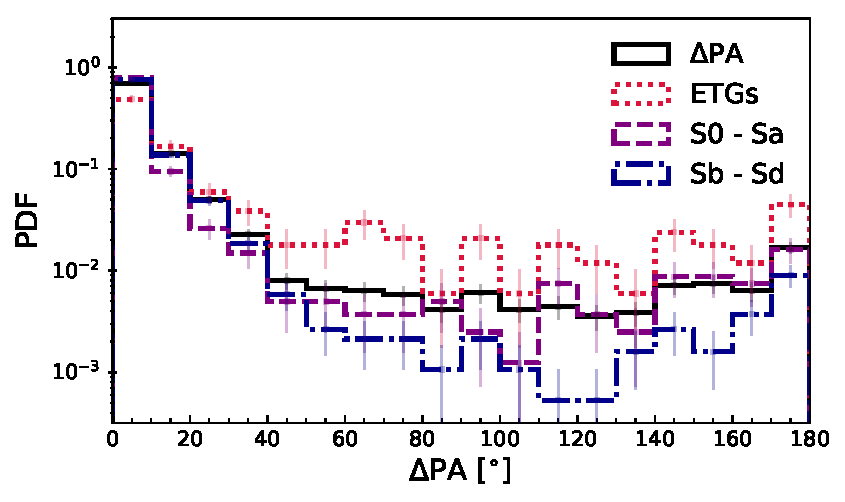
\includegraphics[width=\linewidth]{thesis/latex/misalignment_MaNGA/delPA_morph.pdf}
    \caption{Probability density distributions of kinematic misalignment as defined by $\Delta$PA split on morphology. The probability density distribution is normalised to 1 and shown in log scale. Distributions for the total population, ETGs, S0/Sa and Sb-Sds are shown by black solid, dotted red, dashed purple and dot-dashed blue lines respectively. Earlier type galaxies are more likely to be misaligned than later type galaxies.}
    \label{fig:morph_PA}
\end{figure}

Due to the relationship between stellar mass, morphology and specific angular momentum \citep[e.g.][]{cortese2016}, it might be expected that misaligned galaxies should be at higher stellar mass due to their lower $\mathrm{\lambda_{R}}$ with respect to the aligned \citep[see also;][]{bryant2019}. Surprisingly for the overall population we see little difference, however, splitting on morphology as shown in Figure \ref{fig:morph_stelM} reveals individual trends. Misaligned ETGs (and NGRs) are more massive than the aligned counterparts most likely indicative that misaligned galaxies have had richer merger histories. The opposite trends are seen for both S0-Sas and Sb-Sds with kinematically aligned galaxies being of typically higher mass than the misaligned. This could be indicative that the pathways leading to misalignment are different as a function of morphology.

\begin{figure}
    \centering
	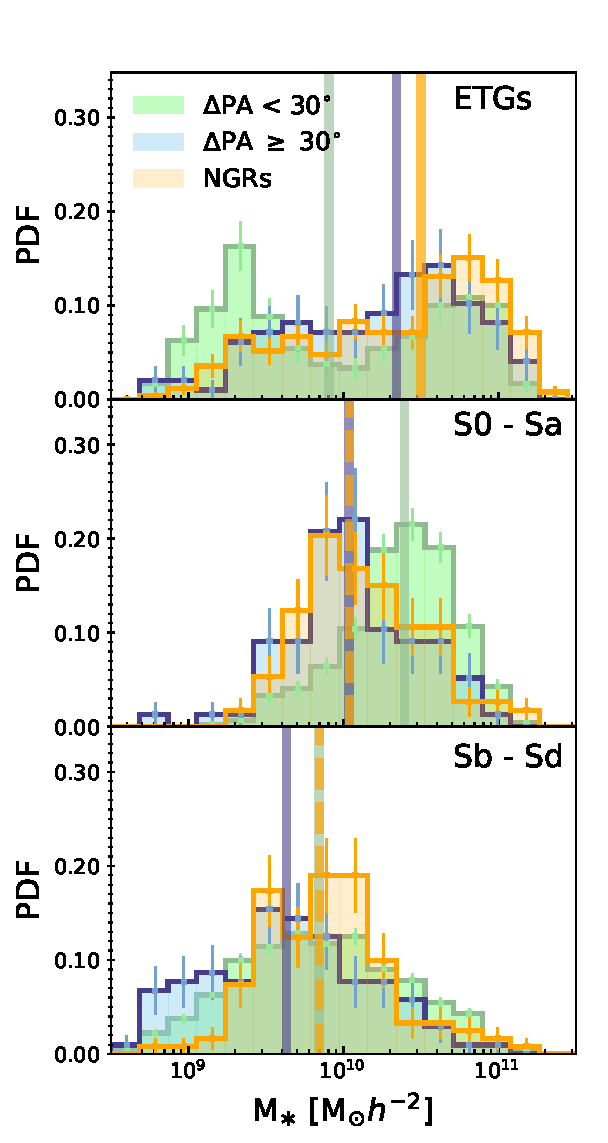
\includegraphics[width=0.5\linewidth]{thesis/latex/misalignment_MaNGA/delPA_stelM_morph_nsa.pdf}
    \caption{Probability density distributions of stellar mass, $\mathrm{(M_{\ast}/M_{\odot})}$ for aligned galaxies ($\Delta$PA < 30$^{\circ}$, misaligned galaxies ($\Delta$PA > 30$^{\circ}$) and NGRs for ETGs, S0-Sas and Sb-Sds (top to bottom). In each panel the aligned/misaligned are shown with solid lines with the aligned in the darker shade. NGRS are shown by dot-dashed lines. Each histogram is given with Poisson errors on each bin. The vertical lines denote the corresponding distribution's median. For ETGs, aligned galaxies are less massive than the misaligned sample. This trend, however, reverses for S0-Sas and Sb-Sds.}
    \label{fig:morph_stelM}
\end{figure}

\subsubsection{Group membership}
Group membership is important for dictating the evolution of a galaxy and hence we now sub-divide our population into centrals and satellites as described in \S\ref{sec:group_def}. Figure \ref{fig:group_morph_PA} (top panels) shows the $\Delta$PA distributions as in Figure \ref{fig:morph_PA}, but now split into centrals and satellites. Qualitatively the morphological trends remain however Table \ref{tab:mega_table} reveals that centrals (29.4$\pm$3.2\%) are slightly more likely to be misaligned than satellites (24.7$\pm$4.4\%) for ETGs. This is also potentially seen for the S0-Sbs (10.1$\pm$1.4\% for centrals vs 8.8$\pm$2.0\% for satellites), however we note that both fractions are within each other's errorbars.

\begin{figure*}
    \centering
	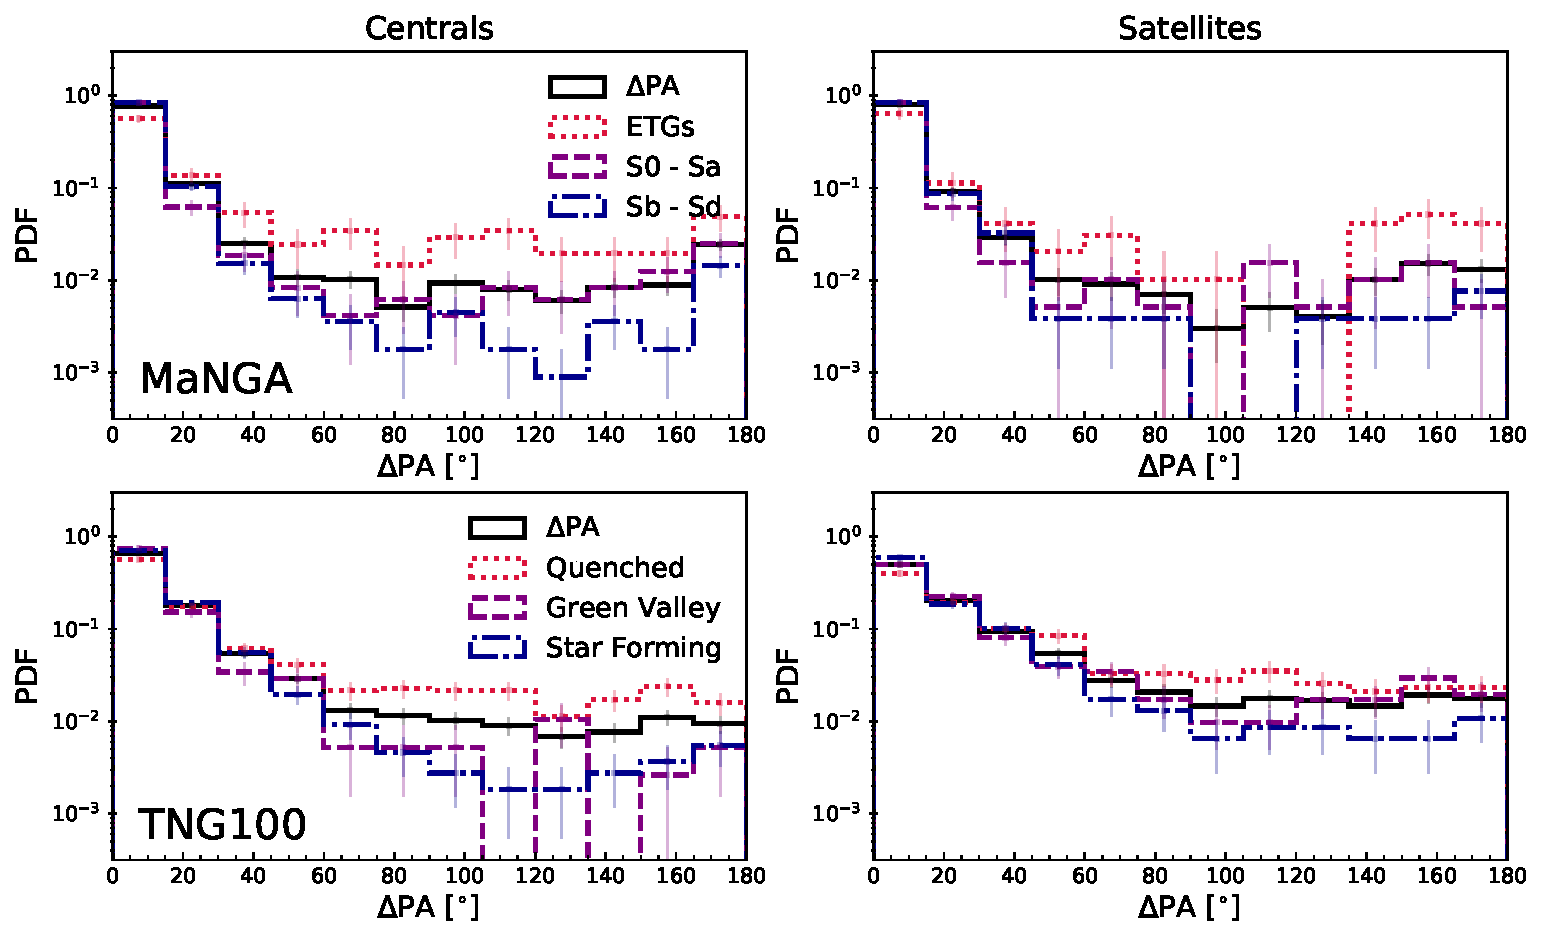
\includegraphics[width=\linewidth]{misalignment_MaNGA/MPL8_TNG_morph_group_PA.pdf}
    \caption{Same as Figure \ref{fig:morph_PA}, however split by group membership into centrals (left) and satellites (right). The top panel shows for the MaNGA sample and the bottom shows for the mock sample in TNG100. Morphology for TNG100 is categorised by the deviation of the galaxy's star formation away from the main sequence of galaxies in the whole of TNG100 (see \S\ref{sec:tng_morph}).}
    \label{fig:group_morph_PA}
\end{figure*}

Figure \ref{fig:group_morph_stelM} shows the stellar mass distribution for our samples but now additionally split into centrals and satellites. Again we find the same qualitative trends for both centrals and satellites; i.e. misaligned ETGs are more massive than their aligned counterparts whereas misaligned S0-Sas and Sb-Sds are less massive than those aligned.
\begin{figure*}
    \centering
	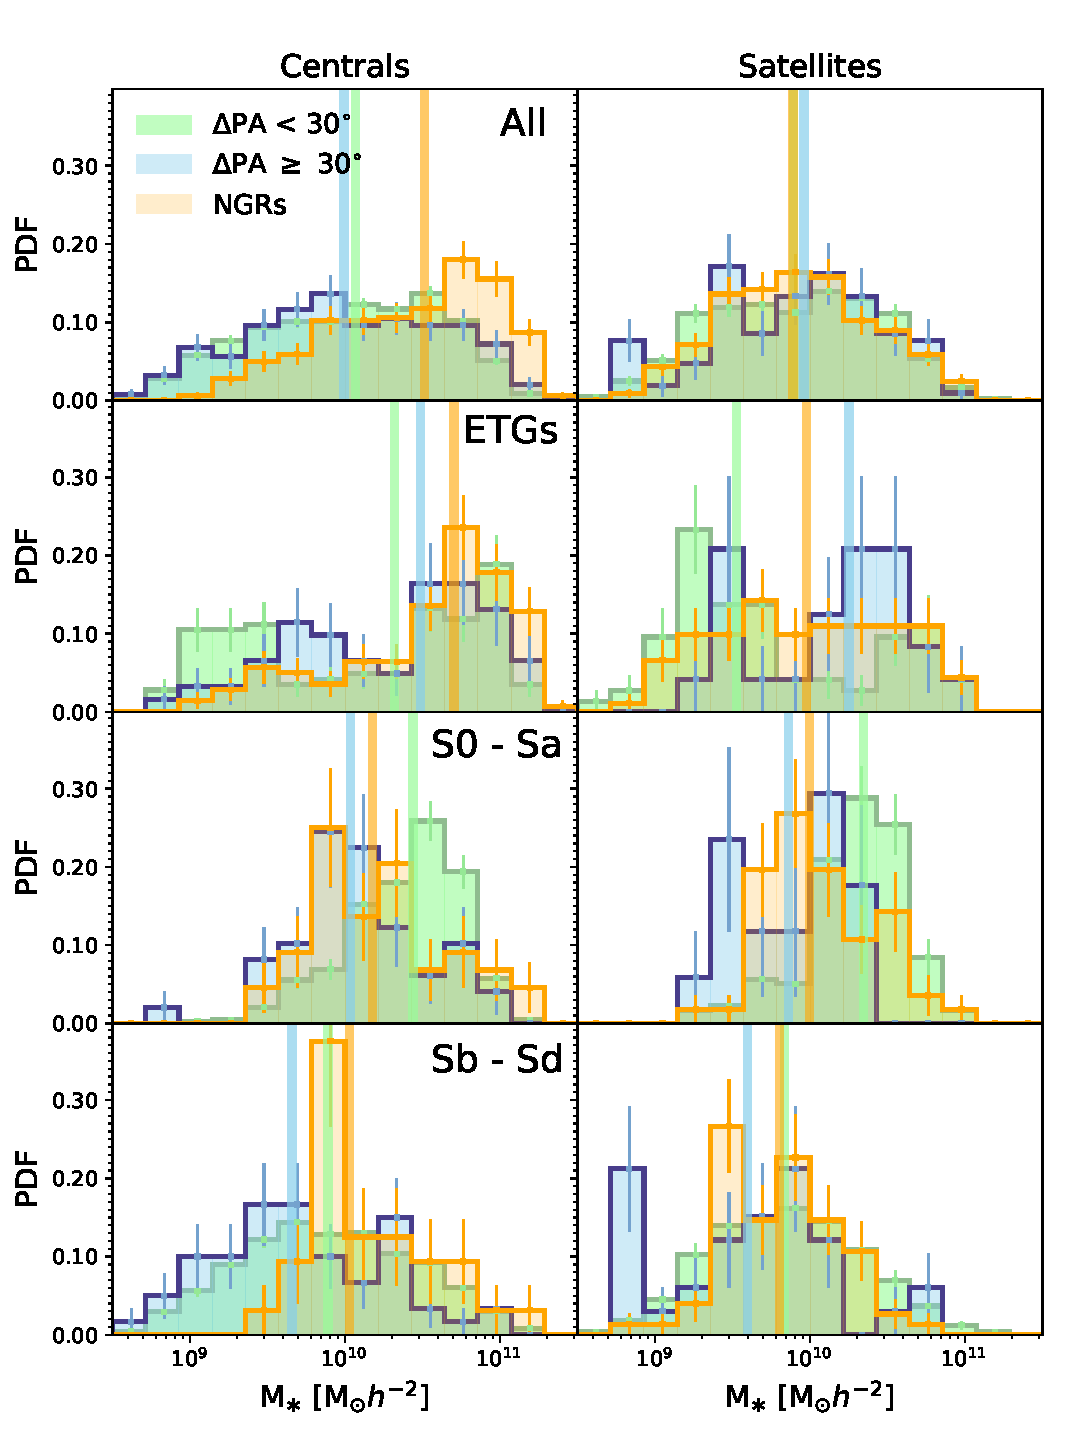
\includegraphics[width=0.85\linewidth]{misalignment_MaNGA/delPA_stelM_morph_lim_nsa.pdf}
    \caption{Same as Figure \ref{fig:morph_stelM}, however split by group membership into centrals (left) and satellites (right). Additionally the distributions for the overall central and satellite populations is shown in the top row. We see that for ETGs there is a strong difference in mass between aligned and misaligned satellites. This trend is reversed for S0/Sa and Sb/Sd satellites. These trends are also seen for centrals, however, typically to a lesser degree.}
    \label{fig:group_morph_stelM}
\end{figure*}

\subsection{Summary of observations} \label{sec:summary_manga}
In the first half of this chapter, we introduce a catalogue of $\sim$4500 galaxies from the MaNGA survey in order to establish the
prevalence of misalignment as a function of optical morphology. We also relate the typical stellar angular momentum and gas content of kinematically misaligned galaxies relative to the aligned. Our conclusions are as follows:

\begin{enumerate}
    \item The prevalence of kinematic misalignment (i.e. where rotational axes of stars and gas are offset by $> 30^{\circ}$) is strongly morphological dependent with $\sim$28\% of ETGs exhibiting misalignment which decreases to $\sim$5\% for Sb-Sds.
    
    \item For all morphologies this misalignment is related to a lowered stellar angular momentum and also a lowered gas mass. We note that misaligned galaxies have similar stellar angular momentum to those do not have coherently rotating gas (those with large gas depletion fall into this category). This could be indicative that galaxies without coherent gas rotation and kinematically misaligned galaxies are different timesteps in the same evolutionary sequence. As noted in simulations \citep[][]{vdvoort2015, starkenburg+19}, a key component in decoupling star-gas rotation is a significant gas loss followed by accretion of new gas with misaligned angular momentum. In this scenario, NGRs could represent an earlier timestamp before a future re-accretion of gas. This would indicate that the stellar angular momentum is disrupted prior to accretion of new material. 
    
    \item We find that the misalignment fraction is also dependent on group membership. For ETGs and S0-Sas, central galaxies are more likely to exhibit misalignment than satellites. For Sb-Sds this trend reverses.
    
    \item We find that counter-rotation (i.e. rotational axes of stars and gas are offset by $> 150^{\circ}$) is a stable state for galaxies of all morphologies shown by a boost in the PDF (Figure \ref{fig:morph_PA}). Similar to the total misaligned population, counter-rotators have distinctly lower angular momentum than their aligned counterparts. 

\end{enumerate}
In the following section, we investigate whether hydrodynamical simulations can reproduce these observed trends and what typical timescales are associated with angular momentum and gas loss.

\section{In IllustrisTNG} \label{sec:tng_kin_mis}
\subsection{Simulation data} \label{sec:sim_data_TNG}
\subsubsection{IllustrisTNG} 
The \texttt{IllustrisTNG} project \citep{marinacci18,naiman18,nelson18,pillepich18b,springel18} is a suite of magneto-hydrodynamic cosmological scale simulations incorporating an updated comprehensive model for galaxy formation physics \citep[as decribed in][]{weinberger17,pillepich18a} and making use of the moving-mesh code \texttt{AREPO} \citep{springel10,pakmor11,pakmor13}. For this work, we use the highest resolution fiducial run of TNG100 which follows the evolution of 2 x 1820$^3$ resolution elements within a periodic cube with box lengths of 110.7 Mpc (75 h$^{-1}$ Mpc). This corresponds to an average mass resolution of baryonic elements of 1.4 x 10$^6 \mathrm{M_{\odot}}$ and 7.5 x 10$^6 \mathrm{M_{\odot}}$ for dark matter. Here we make use of public data from the \texttt{IllustrisTNG} project \citep[as described in][]{nelson2019}.

Structure in TNG100 is identified into haloes and subhaloes as follows. Haloes (also referred to as FoF haloes or Groups) are found from a standard friends-of-friends (FoF) algorithm \citep{davis85} with linking length $b=0.2$. The FoF algorithm is run on the dark matter particles, and the other types (gas, stars, BHs) are attached to the same groups as their nearest DM particle. Each halo is then divided into gravitationally bound subhaloes through the subfind algorithm \citep{springel01}. In short, subfind defines `subhaloes' as locally over-dense and self-bound particle groups as distinct objects within given FoF haloes. We consider all subhaloes at $z=0$ containing a minimum stellar mass of $\mathrm{M_{\ast}} = 10^{8.5} \mathrm{M_{\odot}}$ to potentially make up our mock MaNGA like sample. Since we are typically considering the stellar component of these subhaloes for our mock observations, we will refer to these as TNG100 galaxies.

\subsubsection{Matching to MaNGA sample}
To construct a mock MaNGA sample we select representative subhaloes from TNG100. For every MaNGA galaxy, we find the TNG100 galaxy with the most similar stellar mass, size and SDSS $g - r$ colour. In this instance, stellar mass is defined by the total mass of stellar particles within a radius of 2 stellar effective radii. The SDSS $g - r$ colour is found using the prescription outlined in \citet{nelson18}. Here we describe the general process, while we direct the reader to \citet{nelson18} for more detail. Each stellar particle in the simulation is modelled as a single-burst simple stellar population. This is converted into a population spectrum using \texttt{FSPS} \citep[Flexible Stellar Population Synthesis;][]{conroy2009,conroy2010,foreman_mackey2014} which is convolved with the pass-bands for SDSS colours. We use model C \citep[as described in][]{nelson18} which also includes models for unresolved and resolved dust. We use sizes following the prescription of \citet{genel2018}, which use a projected half light radius. The SDSS bands are constructed as above and are used to define circular half light radii for each SDSS band along X, Y and Z projections of the box. We use the $r-$band half light radius projected perpendicular to the XY plane, consistent with the line of sight of the mock MaNGA observation.

The matching is done through finding the closest neighbour in a normalised space with dimensions of the matched properties. If multiple MaNGA objects match to a given TNG100 galaxy then the absolute nearest neighbour is selected and the MaNGA object is assigned to its second nearest neighbour. The process is iterated until all have unique matches. 

The galaxy is then assigned the same bundle size IFU as the matched MaNGA galaxy with the corresponding angular resolution. The galaxy is then `observed' (see \S\ref{sec:mock_obs}) at a distance so that the angular footprint of the assigned IFU covers the same number of physical effective radii for the mock galaxy as the matched observation. 

\subsubsection{Mock observations} \label{sec:mock_obs}
We convert each galaxy in TNG100 into a mock MaNGA observation, as follows:

We take the raw particle/cell data of stars/gas and project on the XY plane (i.e. z-direction is the line of sight). Since there is no preferred direction in the simulation, this corresponds to a `random' viewing angle of each galaxy. We bin particles corresponding to the angular resolution of spaxels in MaNGA (0.5 arcsec/pixel), in the distinct hexagonal footprint of MaNGA observations. In each bin, we calculate the mean velocity, velocity dispersion and total flux for all particles. Since we include all particles along the line of sight, we must take care in interpreting the absolute values of flux, since none is lost due to obscuration. We, however, do not use the flux values calculated here in our work.

In order to estimate the typical noise associated with a MaNGA observation, we compute radial profiles of the signal to noise ratio (SNR) for all MaNGA observations of a given IFU size. MaNGA has 5 different IFU sizes corresponding to bundles of 19, 37, 61, 91 and 127 fibres. MaNGA provides estimates of the SNR for every spaxel in each observation in the $g$-band. Figure \ref{fig:noise_profile} shows the azimuthally averaged SNR profiles for all MaNGA observations of each fibre bundle size. We fit a logarithmic function to each profile, which is used to assign noise to the mock observations. Noise is drawn for each pixel from a normal distribution using the median and standard deviation of the fitted logarithmic radial profile.

\begin{figure}
    \centering
	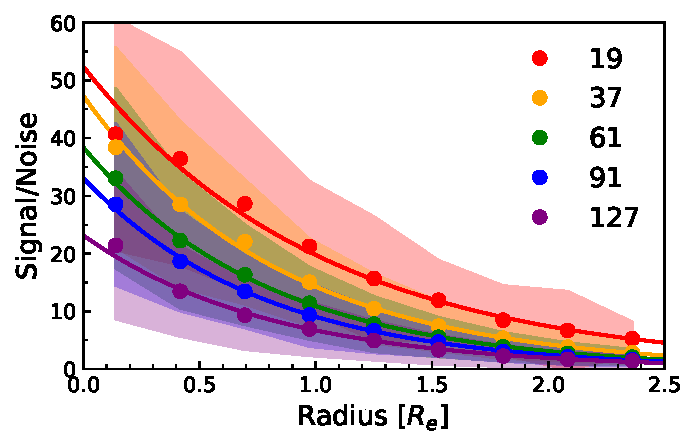
\includegraphics[width=0.95\linewidth]{misalignment_TNG/noise_profiles_ifusize.pdf}
    \caption{Average signal to noise profiles for each IFU size for all MaNGA MPL-8 observations. The circles show the median value for each radius bin with the shaded region corresponding to the standard deviation. The solid line corresponds to an logarithmic parametric fit to the data points, used in sampling the noise profile for the mock observations.}
    \label{fig:noise_profile}
\end{figure}

In order to simulate the effects of the point spread function (PSF), we then convolve our binned particle data with a Gaussian kernel. MaNGA observations typically have a $g$-band PSF which can be fit with a Gaussian of $\sim 2-3''$ full width half maximum (FWHM). We take all our mock observations to have a PSF modelled by a Gaussian with a 2$''$ FWHM. The spatial scale of the simulation is effectively set by the gravitational softening length of both the DM and stellar particles at 0.5h$^{-1}$ kpc = 0.74 kpc. This is approximately a factor of two (four) lower than the spatial sampling (PSF) of a typical MaNGA observation. The typical spatial resolution of star forming gas cells in TNG100 is of order $\sim$200pc and therefore suitable for our mock observations. We direct the reader to Figure 1 in \citet{pillepich2019} for further details (scale by a factor of $16^{1/3}$ for TNG100).

We fit position angles to MaNGA observations that have been Voronoi binned so that bins contain a minimum S/N $\sim 10$. To maintain consistency and avoid spurious individual particles biasing measurements, we also Voronoi bin our mock observations so that a minimum of 5 particles is contained within a given bin, again using the routine of \citet{cappellari2003}. Figure \ref{fig:example_obs} shows example stellar (and gas) velocity and dispersion fields along with normalised $r$-band flux, after our processing. While this is sufficient for the purpose of this work (i.e. fitting kinematic positions to bulk rotation), we recommend the \texttt{SimSpin} package \citep{harborne2019, harborne2020} for detailed mock IFS cube creation.

\begin{figure*}
	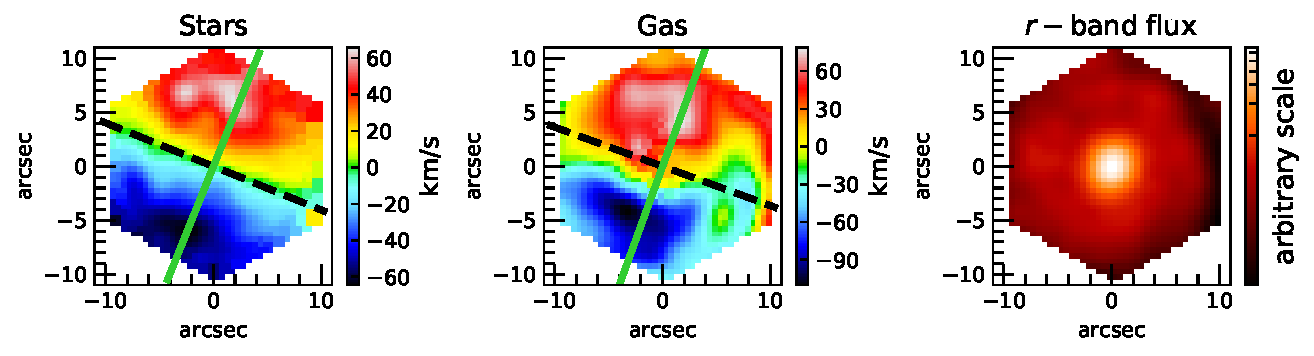
\includegraphics[width=\linewidth]{misalignment_TNG/example_kinematics.pdf}
    \caption{Example outputs from a MaNGA-like observation in TNG100. Shown (left to right) are the stellar velocity field, gas velocity field and normalised $r-$band flux for a given galaxy, `observed' under the same conditions of its MaNGA counterpart (i.e. distance and IFU size). For the stellar and gas velocity fields, the kinematic PA fits are shown (green solid line) with the axis of rotation (black dotted line).}
    \label{fig:example_obs}
\end{figure*}

\subsection{Comparisons to observations} \label{sec:manga_tng_comp}
\subsubsection{$\Delta$PA}
Firstly we consider all $\Delta$PA defined galaxies for both MaNGA and TNG100. Figure \ref{fig:total_pa_dist} shows the distribution of $\Delta$PA for both MaNGA and \texttt{100}. Both distributions are strongly peaked around around 0$^{\circ}$ indicative of the preferentially aligned state predicted from tidal torquing theory. The MaNGA distribution shows a sharp drop-off past 40$^{\circ}$ whereas TNG100 shows a smoother drop off to higher misalignments. Additionally the MaNGA distribution shows a second peak around 180$^{\circ}$ indicative of the stable counter-rotating state identified in previous work \citep[e.g.][]{chen2016}. This secondary peak is not seen for the overall TNG100 sample, however is apparent for central star forming galaxies in TNG100 (see bottom panel of Figure \ref{fig:group_morph_PA}). 

\begin{figure}
    \centering
	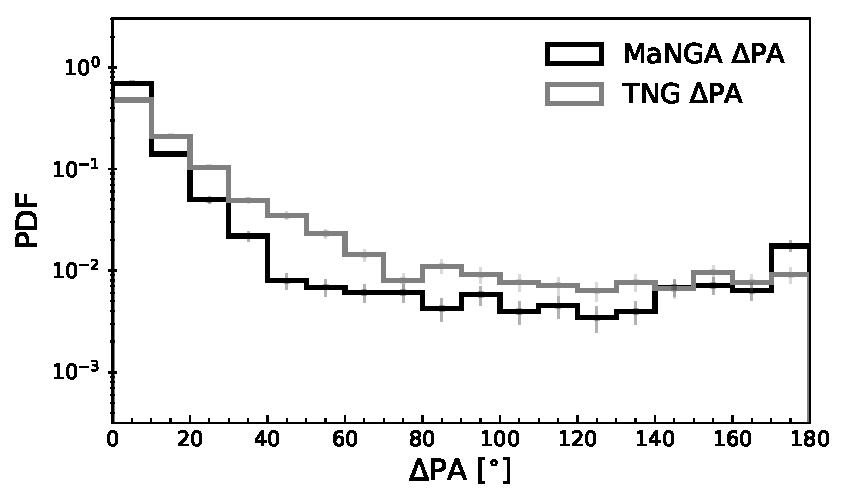
\includegraphics[width=0.85\linewidth]{misalignment_TNG/mpl8_pa_dist.pdf}
    \caption{Probability density distribution of kinematic misalignment as defined by $\Delta$PA for the total MaNGA sample (black line) and matched TNG100 sample (grey line). $\Delta$PA is strongly peaked around 0$^{\circ}$ with a small boost close to 180$^{\circ}$.}
    \label{fig:total_pa_dist}
\end{figure}

The TNG100 mock sample reproduces the general trends well, when considering the differences in how we split the samples in observations and simulations. The smoother drop-off past 40$^{\circ}$ for TNG100 is likely a combination of how we construct the mock observations and scatter in the mass distributions between the MaNGA and TNG100 samples. By construction the matching between MaNGA and TNG100 objects is done before $\Delta$PA is calculated. For this reason there may be differences between the mass distribution of the $\Delta$PA defined MaNGA and TNG100 samples, as shown in Figure \ref{fig:TNG_mpl8_stelM}. We find that the misaligned sample in TNG100 is slightly more massive with respect to MaNGA whereas the aligned samples are consistent. Due to the strong morphological dependence on kinematic misalignment, there is a secondary dependence on stellar mass. The increased overall fraction of misaligned galaxies in TNG100 is therefore, in part, due to the TNG100 $\Delta$PA defined sample being slightly more massive. This slight boost could indicate that the mechanisms for misalignment may be different in simulations than observations. \citet{khim2019} compare the misalignment fractions in observations (SAMI) with simulations (\texttt{Horizon-AGN}). While overall a good agreement is found, they note a significant difference in cluster environments where simulated galaxies are far more likely to be misaligned than in observations. More work needs to be done to understand how well cosmological hydrodynamical simulations replicate the processes leading to misalignment in observations, however, overall trends appear to be well reproduced for different simulation prescriptions.

\begin{figure}
    \centering
	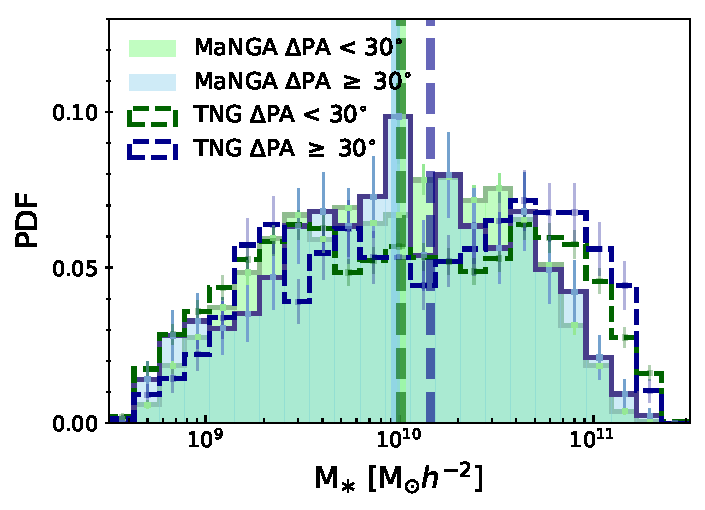
\includegraphics[width=0.85\linewidth]{misalignment_TNG/delPA_split_stelM_tng_comparison.pdf}
    \caption{Probability density distributions of stellar mass, $\mathrm{(M_{\ast}/M_{\odot})}$ for aligned galaxies ($\Delta$PA < 30$^{\circ}$, green) and misaligned galaxies ($\Delta$PA > 30$^{\circ}$, red) defined in MPL-8 (solid lines) and TNG100 (dashed). The vertical lines denote the corresponding distribution's median. The overall distributions are a reasonable match between mocks and observations, with a noted preference for $\Delta$PA defined galaxies at the very high mass end for TNG100. }
    \label{fig:TNG_mpl8_stelM}
\end{figure}

\subsubsection{Morphological dependence} \label{sec:tng_morph}
We divide our mock MaNGA sample based on the instantaneous star formation rate (SFR) of the galaxy. Here, we define SFR for all gas cells within twice the stellar half mass radius of a given galaxy. The star forming main sequence for all galaxies is found by fitting a power law as a function of stellar mass. A galaxy is then flagged into one of three categories; star forming, green valley or quenched depending on its deviation above or below the main sequence \citep{pillepich2019}. The selected deviations from the main sequence are as follows; star forming galaxy: $\mathrm{\Delta \log_{10}(SFR) > −0.5}$, green valley galaxy: $\mathrm{-1.0 < \Delta \log_{10}(SFR) < -0.5}$ and quenched galaxy: $\mathrm{\Delta \log_{10}(SFR) <= -1.0}$.

The bottom panel of Figure \ref{fig:group_morph_PA}, shows the $\Delta$PA distribution for the TNG100 sample split into centrals and satellites. Comparing to the observational sample in the top panel of Figure \ref{fig:group_morph_PA}, the morphological trends remain qualitatively the same with quenched/ETGs (star forming/LTGs) more likely to be misaligned (aligned).

Our choice to compare populations split on visual morphology in observations to SFR in simulations is one of necessity. The aim of this work is to explore the relationship of visual morphology with decoupled rotation. Unfortunately we don't currently have the equivalent classifications in \texttt{IllustrisTNG100}, so use an appropriate proxy. In future work, we will look at the relationship between observations and simulations using machine learning classifications of morphology, however, in the following subsections we follow the evolutionary history of the mock sample split by sSFR.

\subsection{Evolution of angular momentum} \label{sec:tng_ang_mom_evo}
\subsubsection{Magnitudes}
In this section, we consider the angular momentum content of our TNG100 mock sample back to $z=1$ for stars, gas and dark matter individually. The prior time evolution of such properties for each galaxy is followed by considering the main progenitor branch (most massive defined by stellar mass) in the sublink merger trees \citep{rgomez2015}. Angular momentum for our TNG100 galaxies is defined by the intrinsic specific angular momentum of their particles/cells:
\begin{equation}
\mathrm{j_{k} = \frac{1}{\sum_{n} m^{(n)}} \sum_{n} m^{(n)}\boldsymbol{x}^{(n)} \times \boldsymbol{v}^{(n)}}
\end{equation}
where $\boldsymbol{v}^{(n)}$ is the velocity of each particle relative to the centre of mass for the galaxy, $\boldsymbol{x}^{(n)}$ is the position of a given particle with respect to the position of the most gravitationally bound particle in the galaxy and $\mathrm{m^{n}}$ is the particle's mass. We choose this definition since the centre of mass velocity can be biased by structure at large radii in the subhalo/galaxy and hence may spuriously not represent the true rotational centre. $k$ is the particle/cell type referring to either stars, gas or dark matter. For stars and gas this is calculated within a 3D radius equal to the 2D radius corresponding to the angular size of the mock observation. Dark matter is calculated for all particles assigned to the subhalo by the subfind algorithm. 

Figure \ref{fig:sJ_evo} shows the specific angular momentum evolution from $z=1$ for each of stars, gas and DM split on group membership and morphology. We see that similar to the observational sample (see Figure \ref{fig:delPA_lambda_Re}), misaligned galaxies in simulations are significantly lower stellar angular momentum than their aligned counterparts at $z=0$. This is reflected in for each of stars, gas and DM to various degrees for all morphologies and central/satellite definition. Interestingly, while misalignment between stars and gas may itself be a transient property, those misaligned at $z = 0$ reside in dark matter haloes with \textit{fundamentally lower angular momentum} which persists to at least $z = 1$. 

\begin{figure*}
	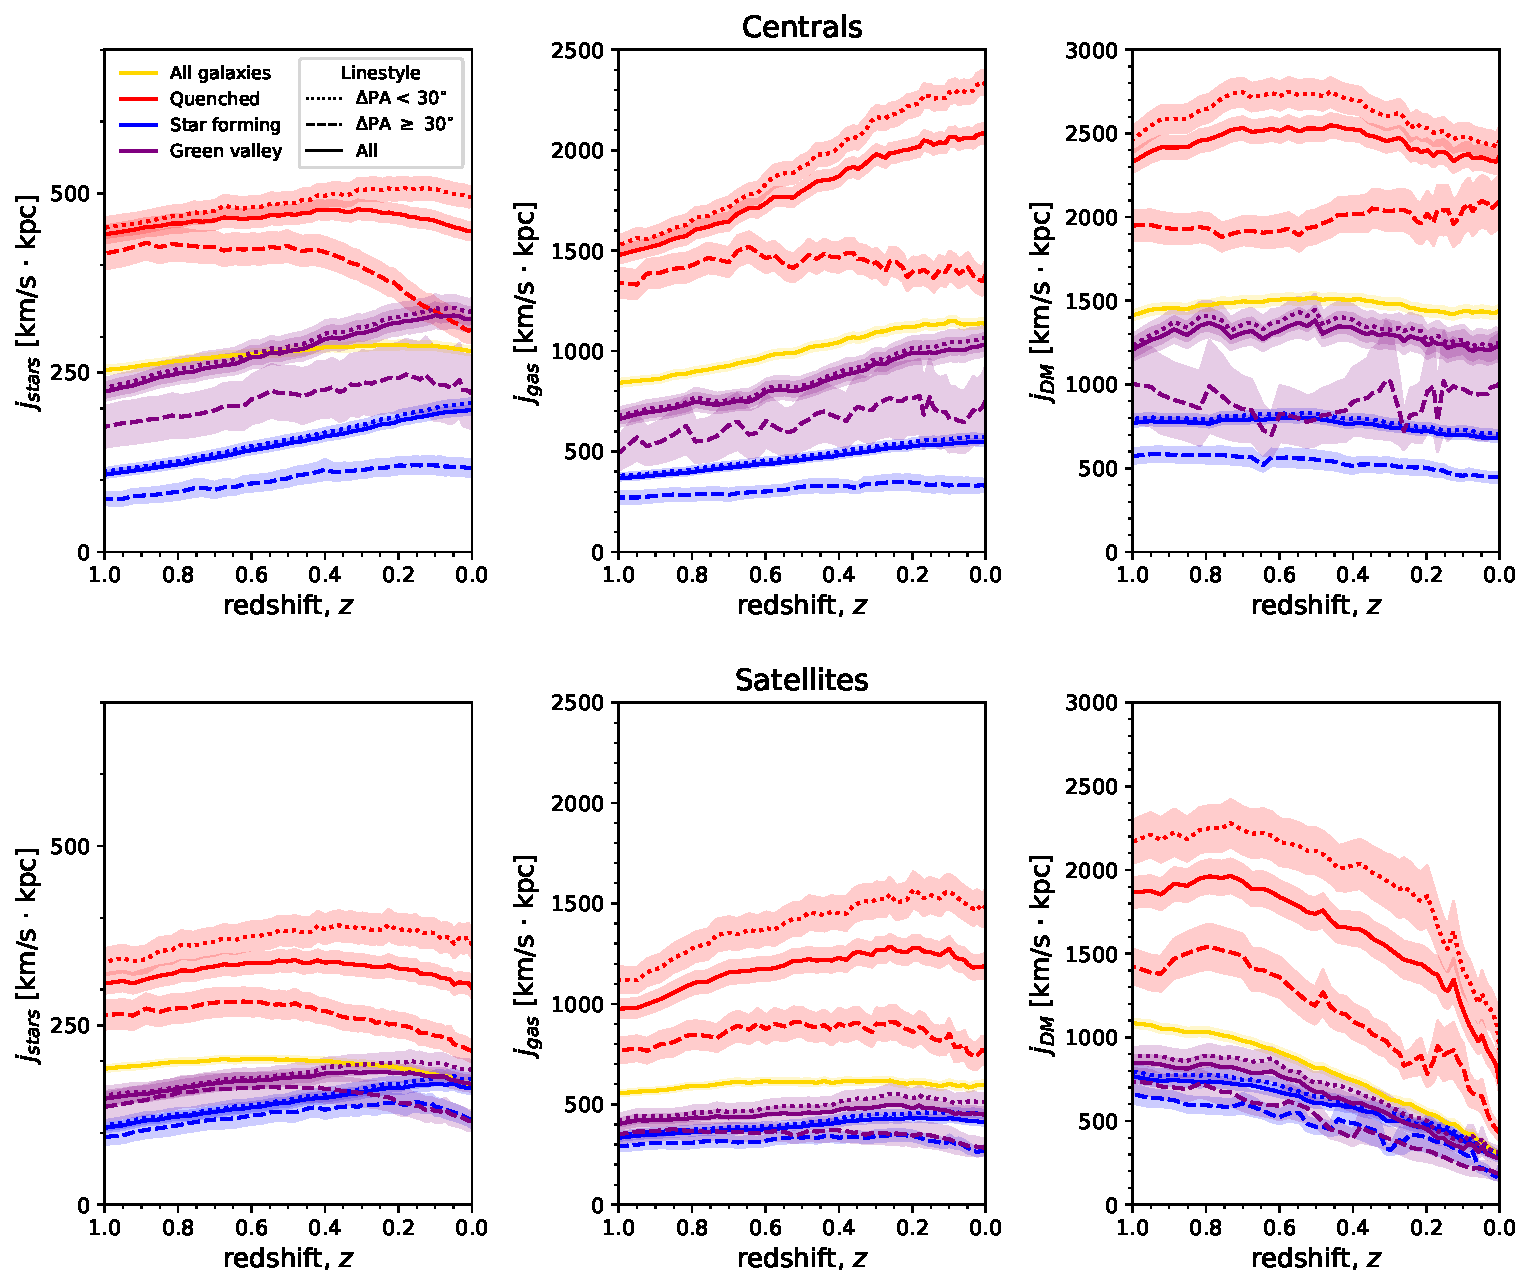
\includegraphics[width=\linewidth]{misalignment_TNG/sJ_evo_cen_sat.pdf}
    \caption{Specific angular momentum evolution from $z = 1$ calculated from star, gas and DM particles (left to right). The angular momentum is calculated for all star and gas particles/cells within the 3D radius assigned by the mock IFU observation, whereas DM is found from all particles associated to the subhalo. The evolution is taken as the median at each timestep for all galaxies of that category with errorbars showing the standard error. The top (bottom) row shows the evolution for central (satellite) galaxies. Each panel displays the evolution split into morphologies; quenched (red), green valley (purple) and star forming (blue) and also $\Delta$PA $< 30^{\circ}$ (dotted) and $> 30^{\circ}$ (dashed). Kinematically misaligned galaxies selected at $z=0$ have notably lower specific angular momentum for all of stars, gas and dark matter.}
    \label{fig:sJ_evo}
\end{figure*}

We note that particle based calculations of specific angular momentum scales with the number of particles (mass). This results in more massive galaxies having higher $\mathrm{j_{i}}$ and further, quenched galaxies (that are typically more massive) having higher $\mathrm{j_{i}}$ than their later type counterparts. While there is only a small difference in-between the mass distributions of our aligned and misaligned samples, to ensure our signal is not simply driven by mass we calculate the residuals of $\mathrm{j_{star}}$ with respect to a typical galaxy of that mass. The residuals, $\Delta \mathrm{j_{star}}$ are calculated by fitting a polynomial to the distribution of $\mathrm{j_{star}}$ vs $\mathrm{M_{\ast}}$ for the galaxies (all mock observations, regardless if $\Delta$PA is well defined) at each snapshot. $\Delta \mathrm{j_{star}}$, is then defined as the deviation of a given galaxy away from the expectation of the fitted line at that mass. Since the trends are qualitatively consistent regardless of morphology, Figure \ref{fig:sJ_evo_residual} shows the specific angular momentum residuals for the total population. For completeness we also include comparison to every galaxy in the mock sample (regardless if $\Delta$PA is well defined). Misaligned galaxies ($\Delta$PA $\geq 30^{\circ}$) for both centrals and satellites show intrinsically lower $\Delta \mathrm{j_{star}}$ with respect to the total population at a given mass, indicative that it is not an effect due to mass. In addition, there is a relative evolution where $\Delta \mathrm{j_{stars}}$ diverges from all galaxies at $z \sim 0.5$ so that misaligned galaxies have even lower stellar angular momentum with respect to the aligned galaxies in recent times.

\begin{figure*}
	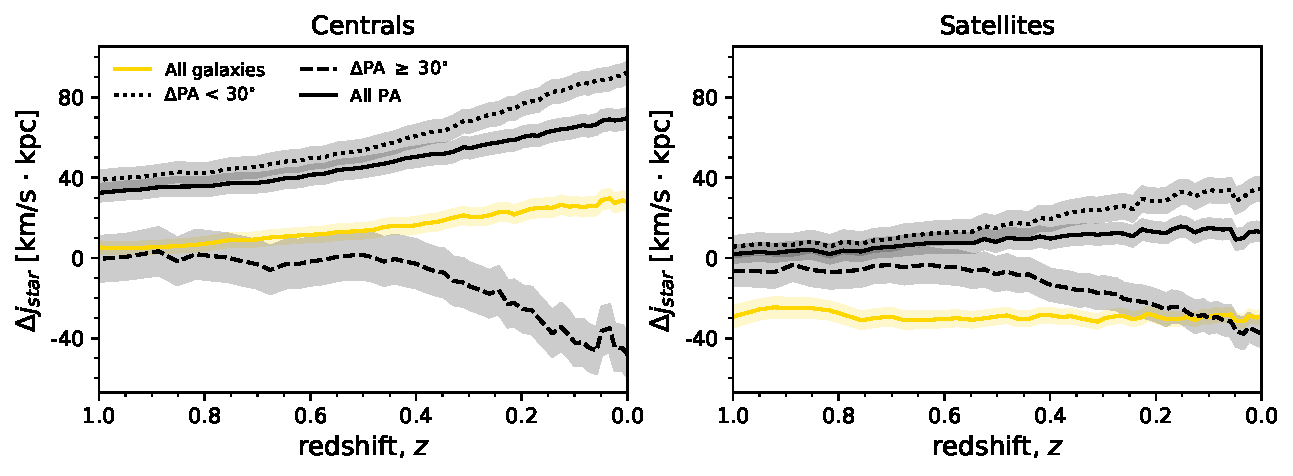
\includegraphics[width=\linewidth]{misalignment_TNG/delta_j_stars_residuals.pdf}
    \caption{The specific angular momentum residuals from $z=1$ for all star particles within the 3D radius assigned by the mock IFU observation. The residual is calculated as the deviation away from the expectation for a galaxy of that mass at each snapshot. The evolution of the residual is taken as the median at each timestep for all galaxies of that category with errorbars showing the standard error. The right (left) panel shows the evolution for central (satellite) galaxies. Each panel displays the evolution for all galaxies (yellow), of which have a defined $\Delta$PA (black solid), aligned galaxies $\Delta$PA $< 30^{\circ}$ (black dotted) and misaligned $> 30^{\circ}$ (black dashed). We see that the difference in angular momentum between aligned and misaligned galaxies is not due to differences in mass. In addition we note a marked deviation of misaligned galaxies to even lower angular momentum in recent times.}
    \label{fig:sJ_evo_residual}
\end{figure*}

\subsubsection{Direction}
\subsubsection{Computation of 3D angles and comparison to $\Delta$PA}
To conclude this section we now consider the directional 3D offsets between the angular momentum vectors of the stars, gas and dark matter. These are calculated from:
\begin{equation} \label{eq:alpha}
\mathrm{\alpha_{3D} = \text{arccos} \left( \frac{\boldsymbol{j_{i}} \cdot \boldsymbol{j_{k}}}{\left| \boldsymbol{j_{i}} \right| \left| \boldsymbol{j_{k}} \right|} \right),}
\end{equation}
where $i, k$ refer to either stars, gas or dark matter. As for the magnitudes of angular momentum, the star and gas vectors are calculated within a 3D radius set to that of the IFU footprint and the dark matter vector is calculated for all particles assigned to the subhalo by subfind.

A key assumption of this work is the ability for the projected $\Delta$PA to be a reliable estimator of the actual 3D offset between star and gas rotation axes. Figure \ref{fig:PA_residual} shows the distributions of the difference between $\Delta$PA and the 2D and 3D offsets between the angular momentum principal axes of stars and gas. The true 3D offset is calculated as in equation \ref{eq:alpha}; the 2D equivalent is simply a projection of this onto the XY plane. $\Delta$PA is a reasonable measure of the true 3D offset which can be modelled as a Gaussian centred on 0$^{\circ}$ with a standard deviation of 17.6$^{\circ}$ (green dotted line). The deviation of the 2D projection from the true 3D offset (black line) has a standard deviation of 13$^{\circ}$, demonstrating that the variation is both due to projection and the noise associated with observations. Additionally, we note the different particle selection for the two measures which may drive slight differences. While the 2D/3D offsets and $\Delta$PA are measured in a footprint with the same radius, the offsets are only defined for particles within a 3D sphere of this radius, where $\Delta$PA is defined for all particles along the line of sight enclosed by the sky footprint. 

\begin{figure}
    \centering
	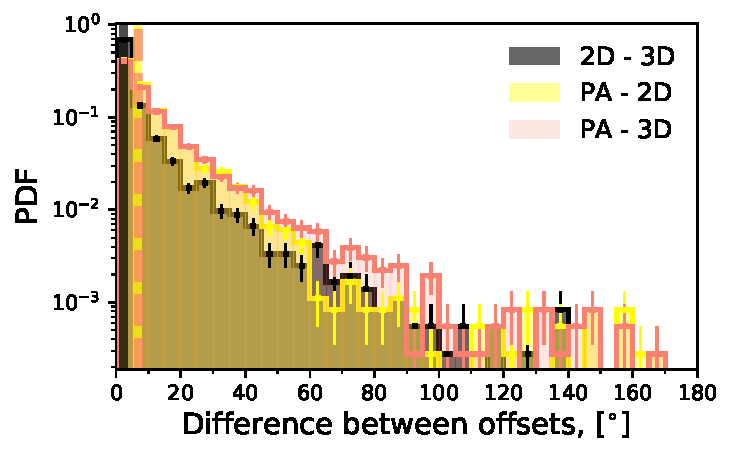
\includegraphics[width=0.7\linewidth]{misalignment_TNG/PA_alpha_resid_hist.pdf}
    \caption{Probability density distribution of the difference between various measures of the star-gas rotational angle offset. The difference between the 3D angular momentum vectors and projection in 2D is shown (black), $\Delta$PA and 2D (yellow) and $\Delta$PA and 3D (red).}
    \label{fig:PA_residual}
\end{figure}

\subsubsection{Results}
Figure \ref{fig:3D_alpha_evo} shows the evolution of the 3D offsets between each of stars, gas and DM respectively. As expected splitting our sample on $\Delta$PA results in significantly higher $\mathrm{\alpha_{STARS - GAS}}$ at $z = 0$ for the misaligned galaxies found in the MaNGA observations. This is also typically correlated, albeit less strongly, with larger $\mathrm{\alpha_{STARS - DM}}$ and $\mathrm{\alpha_{GAS - DM}}$ at $z=0$. This is indicative that a decoupling between stars and gas is often mirrored by a decoupling between the rotation of stars and DM. We also plot the average decoupling for all galaxies (all that are matched to MaNGA) between all components. In the middle panel, we see that $\mathrm{\alpha_{STARS - DM} \sim 50^{\circ}}$ on average for all galaxies (gold line) with a slight redshift evolution which is roughly consistent with previous work \citep[e.g.][]{chisari+17}. We note that our choice to consider the direction of the star and gas rotation within the observational footprint is typically far smaller than the overall DM halo, and hence, may lead to slightly higher typical misalignments between baryonic and DM components.

Working back from $z=0$, we note that $\mathrm{\alpha_{STARS - GAS}}$ for the aligned and misaligned samples (selected at $z=0$) converges in the majority of cases before $z=1$. This indicates the transient nature of misalignment. This is in stark contrast to the magnitude of angular momentum for individual components (stars, gas, DM) which show a persistent difference in magnitude between aligned and misaligned objects (selected at $z=0$) going back past at least $z=1$. 

\begin{figure*}
	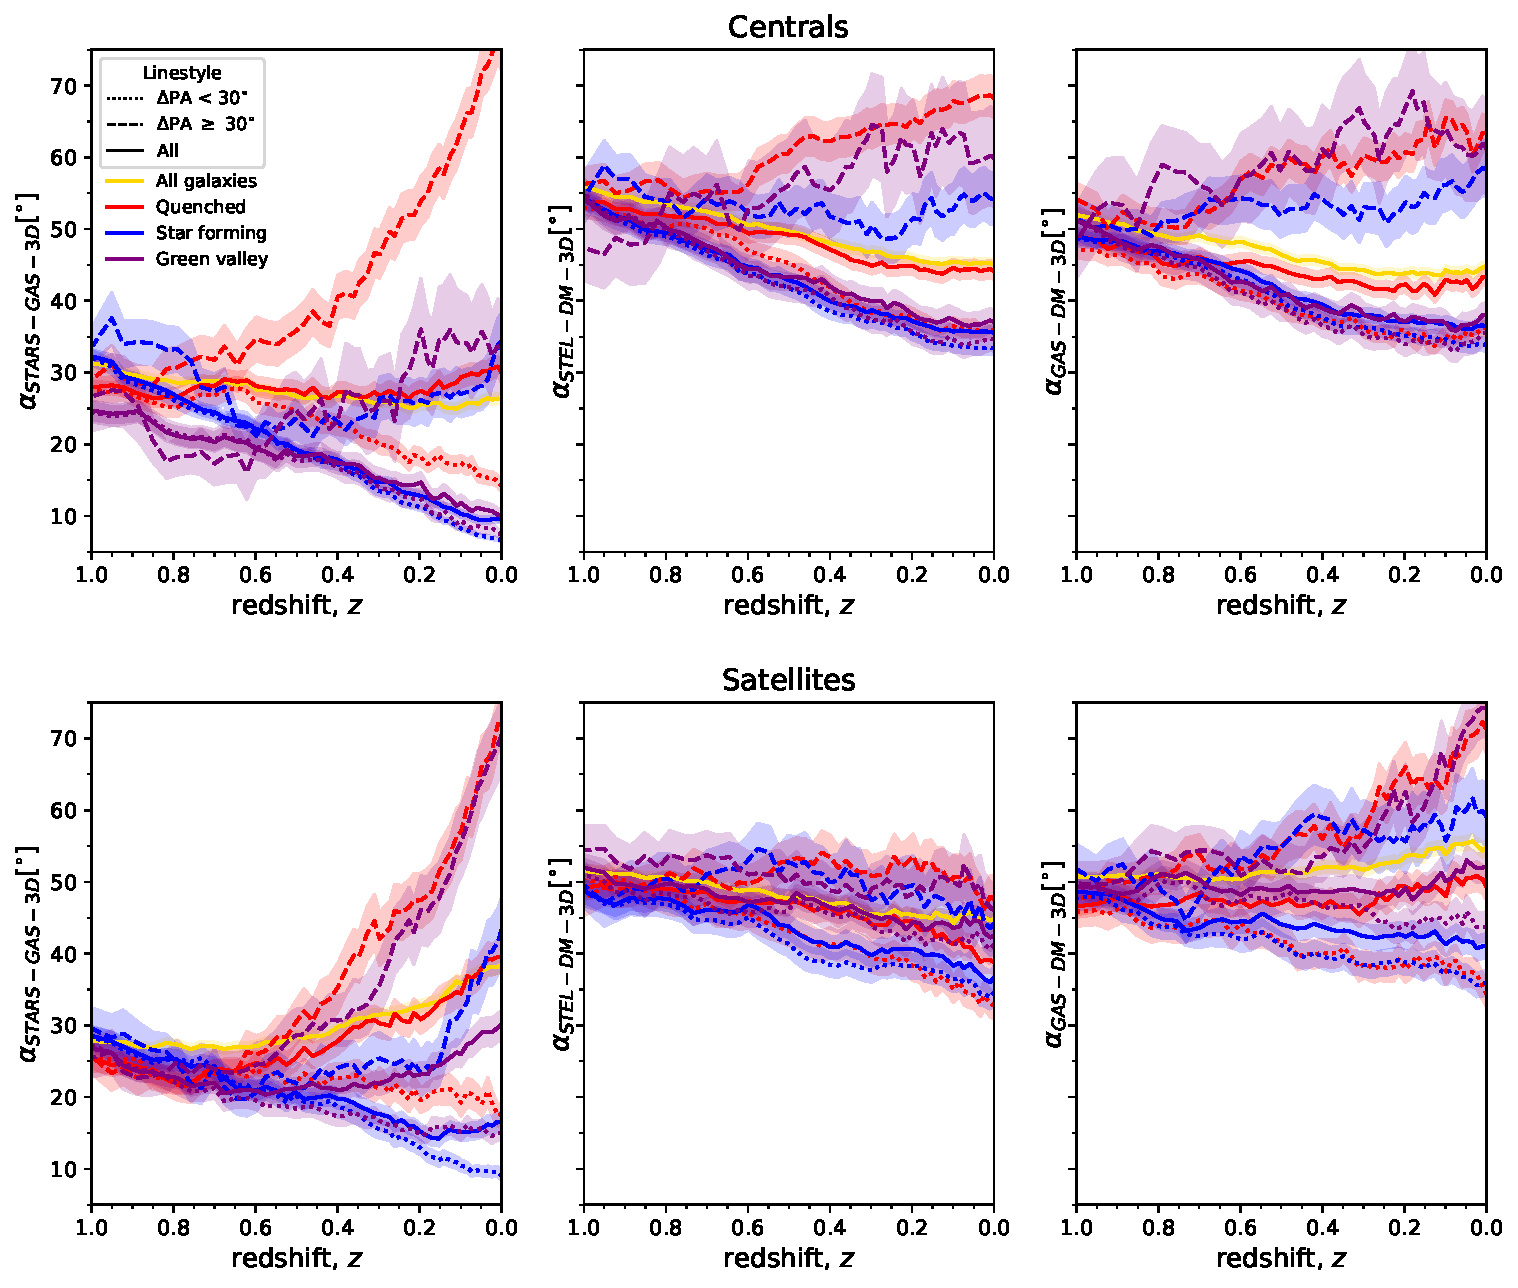
\includegraphics[width=\linewidth]{misalignment_TNG/3D_pa_evo_cen_sat.pdf}
    \caption{Evolution of the 3D offset (in degrees) between the principal spin axes of; stars and gas (left), stars and dark matter (middle) and gas and dark matter (right) from $z=1$. The evolution is taken as the median at each timestep for all galaxies of that category with errorbars showing the standard error. The top (bottom) row shows the evolution for central (satellite) galaxies. Each panel displays the evolution split into morphologies; quenched (red), green valley (purple) and star forming (blue) and also $\Delta$PA $< 30^{\circ}$ (dotted) and $\geq 30^{\circ}$ (dashed).}
    \label{fig:3D_alpha_evo}
\end{figure*}

\subsection{Summary of simulations} \label{sec:tng_summary}
In this chapter, we constructed a mock MaNGA sample in \texttt{IllustrisTNG100} to compare directly to observations and understand the build up of angular momentum in kinematically misaligned galaxies. Our conclusions are as follows:
\begin{enumerate}
    \item We find that a mock MaNGA like sample constructed from cosmological scale hydrodynamical simulation \texttt{IllustrisTNG100} reproduces the observed trends of decoupling with morphology and stellar angular momentum at $z=0$.
    
    \item We find that decoupled galaxies reside in dark matter haloes with lower spin going back past $z=1$. Despite the decoupling between gas and stars being inherently transient in nature, it is also associated with a decoupling of both stars and gas with respect to dark matter. This demonstrates the inherent link of decoupling, not only to present day stellar angular momentum, but to lower spin haloes at $z=1$. 

\end{enumerate}

\section{Discussion} \label{sec:tng_discussion}
In this chapter we have demonstrated the relationship of kinematic misalignment with morphology, stellar angular momentum and dark matter halo spin. In the following we put our results in context and highlight the potential of using the decoupling of star-gas rotation to identify underlying properties of a galaxy. 

We note the close relationship of our findings of our samples with respect to the work of \citet{starkenburg+19}. They investigate the origin of star-gas decoupling (in this instance $ > 90^{\circ}$) using low mass galaxies (i.e. $2 \times \mathrm{10^{9} < M_{\ast} < 5 \times 10^{10}}$) in the original Illustris simulation. Despite extending the mass range and only considering the ensemble average for aligned and misaligned galaxies split at $\Delta$PA$ = 30^{\circ}$, we still find the same qualitative trends of lower angular momentum and lower gas mass fractions for misaligned galaxies (in comparison to aligned). 

While outside the scope of this work, we note that their estimation of relaxation timescales (i.e. until realignment of rotation axes) is of the order Gigayears. This appears to be roughly comparable to toy-model estimates \citep[see;][albeit for ETGs]{davis2016}. Here we also demonstrate the transient nature of star-gas decoupling (left panels, Figure \ref{fig:3D_alpha_evo}). Working back from $z=0$, we note that $\mathrm{\alpha_{STARS - GAS}}$ for the aligned and misaligned samples (at $z=0$) converges in the majority of cases before $z=1$. Since we are only considering the ensemble average for misalignment selected at $z=0$, we cannot comment on the timescales of misalignment here since the average may include several events that decouple the rotation.

In contrast, we see that the magnitude of specific angular momentum for stars, gas and DM for misaligned objects (at $z=0$) remains fundamentally lower going to at least $z=1$. This suggests that while star-gas misalignment at $z=0$ is a transient property, \textit{its likelihood is correlated with the angular momentum content of the halo at early times}. In part, the correlation must be driven by the lower angular momentum content of the stellar component. This inherently leads to longer relaxation timescales (i.e. longer star-gas decoupling) due to weaker stellar torques acting on the misaligned gas component and hence a higher likelihood of being misaligned at $z=0$.

We note the apparent relationship of misalignment with the different evolution of low and high spin haloes due to environment. In Horizon-AGN, \citet{khim2019} show that the misalignment fraction strongly increases in cluster environments. While not explicitly shown in this work, we find that misaligned satellites are typically closer to group centres, indicating the importance of gas stripping or interactions. In observations, \citet{li2019} find that at least 40\% of misalignment can be attributed to recent mergers or interactions. The environment of a given galaxy, modulating the probability of mergers/interactions and hence the spin of the halo/galaxy appears to be an important factor in dictating the misalignment fraction. However, current studies of the environmental dependence of misalignment in observations are inconclusive \citep[e.g. preference for misalignment in overdensity vs isolation; Chapter 5 vs][]{jin2016}.

We also note TNG100's ability to not only reproduce a reasonable distribution of $\Delta$PA with respect to the MaNGA sample (Figure \ref{fig:total_pa_dist}) once accounting for variances in mass between the $\Delta$PA defined samples in MaNGA and TNG100, but also reproducing the strong trends with morphology found in observations (Figure \ref{fig:group_morph_PA}). Whether the trigger of misalignment is internal or external, it appears to be clearly linked to a lowered gas mass (Figure \ref{fig:delPA_gasM}). In the next chapter, we use our simulated sample to investigate the temporal connection between black hole activity and misalignment in \texttt{IllustrisTNG100}. 
\colorlet{chaptergrey}{gray}
\chapter[Kinematically misaligned galaxies in IllustrisTNG]{Kinematic misalignment in TNG}
\label{ch:halo_assembly}
\vspace{-5.25in}
\includegraphics[height=1.39in]{thesis/latex/misalignment_intro/kin_mis_chapter_heading_grey.pdf}
\vspace{3in}

\epigraph{This chapter is based on Duckworth, Tojeiro and Kraljic, in MNRAS, XXX, Issue X, 2020 and Duckworth, Starkenburg, Genel, Davis, Habouzit, Kraljic and Tojeiro (submitted). Here we investigate kinematically misaligned galaxies in the cosmological scale simulation IllustrisTNG. We make direct comparison to observations and investigate the relationship of misalignment identified at $z=0$ with the evolutionary histories of halo spin, gas properties and AGN feedback.}

\section{Introduction}
\colorlet{chaptergrey}{gray}
\chapter[Misalignment and black hole activity]{Misalignment and black hole activity}
\label{ch:halo_assembly}
\vspace{-5.25in}
\includegraphics[height=1.39in]{thesis/latex/misalignment_MaNGA/kin_mis_chapter_heading_grey.pdf}
\vspace{3in}

\epigraph{This chapter is based Duckworth, Starkenburg, Genel, Davis, Habouzit, Kraljic and Tojeiro (submitted). Here we investigate the temporal relationship between kinematically misaligned galaxies and black hole activity in IllustrisTNG.}

\section{Introduction}
Recent cosmological scale hydro-dynamical simulations have provided a clear insight into the relationship between the angular momentum of baryons and dark matter through cosmic time. A necessary component of realistic simulations is efficient feedback from both supermassive black holes (BH) and stars, required to, amongst other things, reproduce late type disks and solve the problem of catastrophic angular momentum loss \citep[e.g.][]{zavala2008, scannapieco2009}. Active galactic nuclei (AGN) and supernova explosions can also lead to dramatic redistribution of gas which regulate the angular momentum content of galaxies \citep[e.g.][]{genel2015, DeFelippis2017}.

`Quasar' (radiative) mode feedback releases huge amounts of energy through radiation from the accretion disk leading to high luminosity AGN and dramatic gas outflows \citep[e.g.][]{cattaneo2009, rubin2014, cheung2016}. Alternatively `radio' (kinetic) mode a term for lower luminosity AGN that host lower black hole accretion rates. In this instance energy is deposited into the surrounding gas via jets which drive outflows, heat the gas and suppress star formation \citep[][]{binney1995, ciotti2001, heckman2014}.

The relationship between AGN and kinematics has been the focus of several recent studies using data from Integral Field Spectroscopy. In particular, a potential new class of galaxy termed `red geyser' has been identified which host AGN and exhibit high velocity outflows in the spatial distribution of ionized gas \citep[][]{cheung2016, roy2018}. These outflows are often linked to a distinctive offset in rotation direction between the stars and gas. Detection of ongoing outflows is, however, rare ($\sim5-10$\% of the quiescent population). \citet{penny2018} demonstrate the importance of AGN feedback in low mass quiescent galaxies ($\mathrm{M_{stel} < 5 \times 10^{9}M_{\odot}}$). While the majority demonstrate no ionized gas present, quiescent galaxies (i.e. with reduced or null SFR) with an AGN show a clear decoupling in the rotation of stars and gas. However, the relationship of gas kinematics to BH feedback is not clear for all galaxies \citep[see also:][]{koudmani2019}. In particular, \citet{ilha2019} find that the typical decoupling between stars and gas for AGN defined galaxies are consistent with an inactive control sample. 

As introduced in chapter 2, the decoupled rotation of stars and gas can be a natural result of external processes \cite[e.g.][]{davis2011, barrera2015, vdvoort2015, jin2016, bryant2019, duckworth2019_halo, li_decoupling2019}. Regardless of internal or external origin, kinematic misalignment in observations and simulations is linked with both a lower gas mass fraction and angular momentum as demonstrated in chapter 3 \citep[see also;][]{starkenburg+19, khim2019}. In particular, \citet{starkenburg+19} highlight the importance of feedback leading to gas loss, enabling new or re-accretion as a mechanism for future misalignment in low mass galaxies. The question arises if misalignment is caused in the first instance by mergers or cosmic gas accretion (and hence making BH accretion easier) or if they are a result of AGN feedback leading to gas loss allowing for accretion of misaligned gas. The timescales of luminous AGN are typically much shorter than kinematic misalignment, making correlation at $z=0$ alone difficult. 

\red{Add section which talks about relationship between major mergers and AGN activity; Hewlett 2017, Ilha 2019 \& associated references?}

In this chapter, we study the temporal relationship between BH feedback, BH luminosity and kinematic misalignment in the cosmological scale hydrodynamical simulation of IllustrisTNG100 (hereafter referred to as TNG100). We use our sample of galaxies with mock MaNGA observations introduced in Chapter 3 to emulate what we may expect to see in IFS observations. In Section \ref{sec:methods_BH} we briefly introduce the specific methods associated with this work, before introducing results in Section \ref{sec:results_BH}. Finally we summarise the chapter in Section \ref{sec:summary_BH}.

\section{Methods} \label{sec:methods_BH}
As introduced in \S\ref{sec:sim_data_TNG}, we make use of data from the IllustrisTNG100 simulation. Black holes are populated in IllustrisTNG based on the mass of the host halo. All haloes without BHs that have a mass greater than $\mathrm{M_{h,thres} = 7.38 x 10^{10} M_{\odot} }$ are automatically populated by a BH of mass $\mathrm{M_{BH} = 8 x 10^{5} h^{-1}}$ at their centre \citep[termed halo-based BH formation, see also;][]{sijacki2009, dimatteo2012, hirschmann2014, sijacki2015}. After being seeded, BHs grow from their seed mass through accretion and BH-BH mergers. BH accretion in IllustrisTNG is modelled by the commonly assumed Bondi formalism. The formalism assumes spherical accretion onto a compact object travelling through the interstellar medium. The accretion rate onto the BH is then assumed to take the form;
\begin{equation}
\mathrm{\dot{M}_{bondi} = \frac{4\pi G^{2} M_{BH}^{2} \bar{\rho}}{\bar{c^{3}_{s}}}}
\end{equation}
where $G$ is the gravitational constant, $c_{s}$ is the sound speed and $\rho$ is the ambient density. This accretion rate in TNG is capped at the Eddington limit (i.e. where there is a balance between the outward force of radiation and gravitational force of in-fall) so that;
\begin{equation}
\mathrm{\dot{M}_{Edd} = \frac{4\pi M_{BH} m_p}{\epsilon_r \sigma_T c} }
\end{equation}
remains an upper bound. Here $\sigma_T$ is the Thomson scattering cross-section for the electron, $m_p$ is the mass of a proton, $c$ is the speed of light and $\epsilon_r$ is the radiative efficiency. Outside of accretion, BHs gain mass through mergers when they come within the feedback radius (i.e. the radius at which the thermal energy is released) of another. One final detail is that BHs in TNG are enforced to remain in minimum of the potential within the haloes they populate. This is done through repositioning of the BH at each timestep so that it remains maximally gravitationally bound. In dramatic events such as galaxy mergers, BHs can be stripped and removed from haloes, however. 

For studies of black hole feedback, of particular relevance is the prescription of \citet{weinberger17} for BH/AGN feedback in TNG100, which is modelled by two distinct modes depending on the current rate of accretion. This choice is reflected in multiple recent cosmological simulations \citep[][]{sijacki2007, dubois2014}, however is not always taken \citep[e.g.][]{schaye2015}. The high accretion state is often associated with luminous quasars at high redshift, and hence is often referred to as `quasar' mode feedback. The feedback is purely thermal and isotropically heats the surrounding gas around the BH. Moving towards lower redshift, BHs are typically accreting at lower rates (i.e. significantly lower than the Eddington limit) and are modelled to be radiatively inefficient. In the original Illustris cosmological simulation feedback in this mode was implemented through injections of bubbles into the surrounding gas \citep{sijacki2007}; however this was updated in IllustrisTNG to a kinetic wind model \citep{weinberger17}. The kinetic mode of feedback (also commonly referred to as radio mode), injects kinetic energy (momentum) in randomised directions. 

The feedback mode is determined by a combination of the instantaneous accretion rate onto the BH and the BH mass. The transition threshold in terms of the Eddington ratio is 
\begin{equation}
\mathrm{f_{Edd}= \min ( 2x10^{-3}(M_{BH}/10^8 M_{\odot})^2 , 0.1)}
\end{equation}
so that BHs typically transition from quasar to kinetic mode around $\mathrm{M_{BH} = 10^{8}M_{\odot}}$. In the following, we separate our TNG100 galaxies by stellar mass at $\mathrm{M_{stel} = 10^{10.2}M_{\odot}}$ (nominally referred to low and high mass galaxies henceforth) which corresponds to this transition \citep[i.e. $\mathrm{M_{BH} \approx 10^{8}M_{\odot}}$, see Fig 1 in][]{li2019}. We do not explicitly follow the individual modes of accretion and feedback for each galaxy, which can alternate through its evolutionary history. Despite this, the transition threshold in TNG determines that we almost exclusively isolate the role of radiative feedback for our low mass sample. Our high mass sample, however, has been subject to both quasar and kinetic feedback over the last 8 Gyrs. To emulate what we may expect to see in IFS observations, we make use of our mock MaNGA sample as introduced in \S\ref{sec:mock_obs}.

Bolometric BH luminosities in cosmological simulations are typically estimated using an expression involving the instantaneous accretion rate onto the BH and the radiative efficiency of the feedback. Historically, BH bolometric luminosities are found by the following expression;
\begin{equation}
\mathrm{L_{bol, AGN}} = \frac{\varepsilon_r}{1 - \varepsilon_r} \dot{\mathrm{M}}_{\mathrm{BH}} \mathrm{c^2}
\end{equation}
where $\varepsilon_r=0.1$ is the radiative efficiency \citep[see discussion in][]{habouzit2019}, c the light speed, and $\dot{\mathrm{M}}_{\mathrm{BH}}$ the accretion rate onto the BH. Here we adopt the same expression. In addition to BH properties, in this chapter, the time evolution of gas properties are also presented. Gas properties are defined within two effective radii ($\mathrm{R_{e}}$, radius containing half of the stellar mass within the galaxy), unless stated otherwise.

\section{Results} \label{sec:results_BH}
Each panel of Figure \ref{fig:overall_pop} shows the time evolution average of a property for all galaxies split by stellar mass at $\mathrm{M_{stel} = 10^{10.2}M_{\odot}}$, as explained in \S\ref{sec:methods_BH}. Splitting directly on BH mass at $\mathrm{M_{BH} = 10^{8}M_{\odot}}$ or enforcing stricter stellar mass cuts does not change any of our findings. We divide our sample by $\Delta$PA at $z=0$. For each sub-population, we find that the stellar mass distributions are consistent at $z=0$ for aligned and misaligned galaxies. Equivalent to our selection in chapter 3, we also split on specific star formation rate using the distance from the star-forming sequence (SFS) as defined in \citet{pillepich2019}. We select star forming ($\Delta \mathrm{log_{10}(SFR) > -0.5}$) and quenched galaxies ($\Delta \mathrm{log_{10}(SFR) \leq -1.0}$) at $z=0$. For clarity, the correlations with each misaligned sub-population in Figure \ref{fig:overall_pop} are summarized by Table \ref{tab:truth}. Additional time evolution properties can be found in Figure \ref{fig:overall_pop_additional}, and are also summarized in Table \ref{tab:truth}.

\begin{figure}
	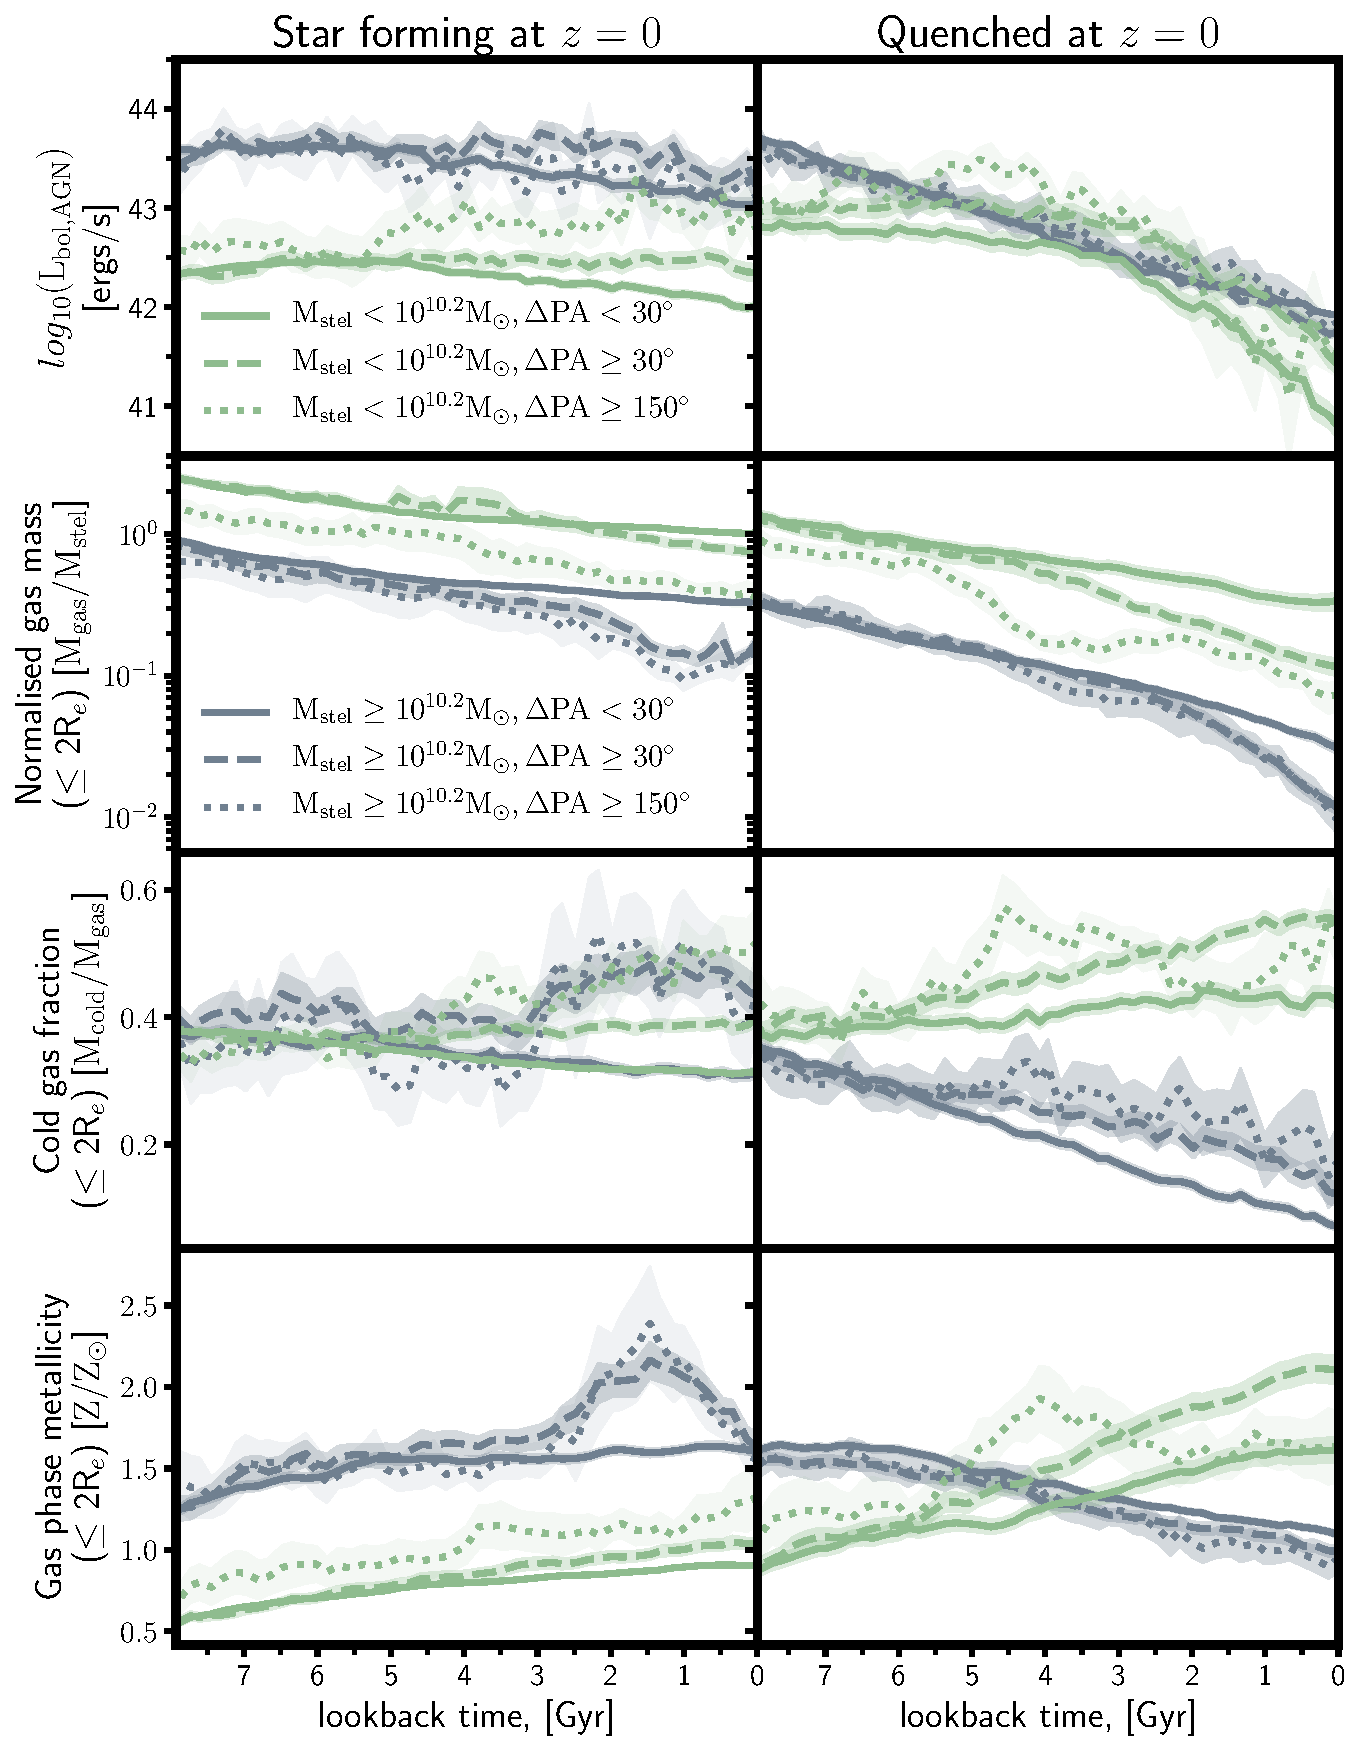
\includegraphics[width=\linewidth]{misalignment_BH/time_evo_letter_without_BH_props.pdf}
    \caption{Time evolution of (rows top to bottom) black hole luminosity ($\mathrm{log_{10}(L_{bol, AGN})}$), normalised gas mass ($\mathrm{M_{gas}/M_{stel}}$), cold and star forming gas fraction ($\mathrm{M_{cold}/M_{stel}}$), and, gas phase metallicity for star forming (left) and quenched galaxies (right) identified at $z=0$. Galaxies are divided into low mass (green; $\mathrm{M_{stel} < 10^{10.2}M_{\odot}}$) and high mass (grey; $\mathrm{M_{stel} > 10^{10.2}M_{\odot}}$) populations. Both are subdivided by misalignment ($\Delta$PA $< 30^{\circ}$: solid, $\geq 30^{\circ}$: dashed, and  $\geq 150^{\circ}$: dotted). Each line shows the mean for the population with the shaded region corresponding to the standard error.}
    \label{fig:overall_pop}
\end{figure}

\begin{figure}
	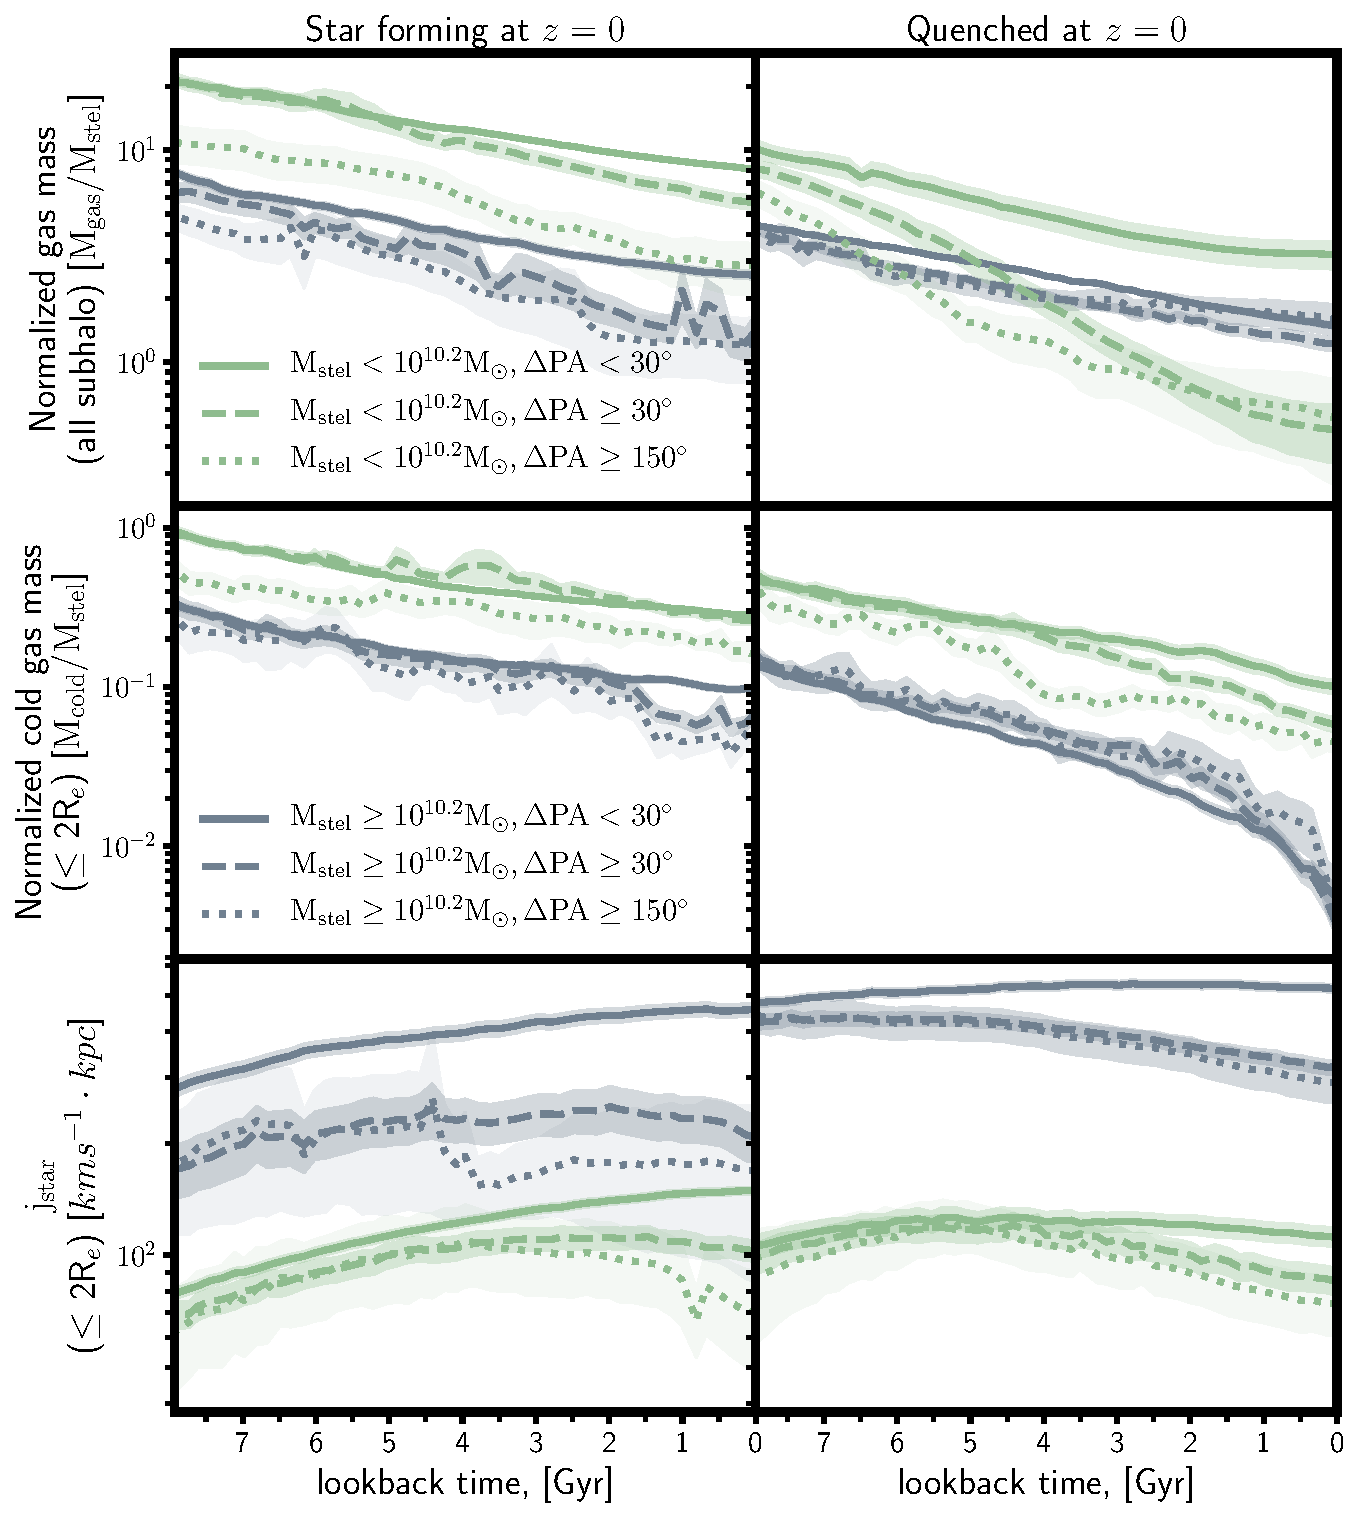
\includegraphics[width=\linewidth]{misalignment_BH/time_evo_supplement_no_feedback.pdf}
    \caption{Time evolution of (rows top to bottom) of normalized gas mass within the total subhalo ($\mathrm{M_{gas}/M_{stel}}$), normalized cold gas mass ($\mathrm{M_{cold}/M_{stel}}$) and specific stellar angular momentum ($\mathrm{j_{star}}$), for star forming (left) and quenched galaxies (right) identified at $z=0$. We show both low mass (green; $\mathrm{M_{stel} < 10^{10.2}M_{\odot}}$) and high mass (grey; $\mathrm{M_{stel} > 10^{10.2}M_{\odot}}$) galaxies. Both are subdivided by misalignment ($\Delta$PA $< 30^{\circ}$: solid, $\geq 30^{\circ}$: dashed, and  $\geq 150^{\circ}$: dotted). Each line shows the mean for the population with the shaded region corresponding to the standard error.}
    \label{fig:overall_pop_additional}
\end{figure}

\begin{sidewaystable}
\centering
\begin{tabular}{llllllll}
\hline
&  $\mathrm{L_{bol,AGN}}$ & $\mathrm{M_{gas} / M_{stel} (< 2R_e)}$ & $\mathrm{M_{cold} / M_{gas}}$ & $\mathrm{Z / Z_{\odot}}$ & $\mathrm{M_{gas}/M_{stel} (total)}$ & $\mathrm{M_{cold}/M_{stel}}$ & $\mathrm{j_{star}}$ \\
\hline
Low mass star forming & ++ & $--$ & ++ & + & $--$ & 0/$-$C & $--$ \\
High mass star forming & + & $-$/bump & ++/bump & ++/bump & $--$ & -/bump & $--$ \\
Low mass quenched & +/bumpC & $--$/bumpC & ++/bumpC & ++/bumpC & $--$ & $--$ & $--$ \\
High mass quenched & 0 & $-$ & ++ & 0$-$ & 0 & 0+ & $--$ \\
\end{tabular}
\caption{Truth table summarising the correlations found in Figure \ref{fig:overall_pop} between BH luminosity, normalised gas mass ($\mathrm{< 2R_e}$), cold gas fraction and gas phase metallicity (first four columns) with misalignment identified at $z=0$. The latter three columns additionally show the correlations found in the Supplementary material between total normalised gas mass (in subhalo), normalised cold gas mass and specific stellar angular momentum with misalignment. Correlations are shown individually for misaligned galaxies separated by both stellar mass and SFR at $z=0$. ++, + ($--$, $-$) refer to strong and mild positive (negative) correlations, 0 to no correlation and bump indicates a feature in the curve. A C is appended if the correlation/feature is only applicable to counter-rotating galaxies.}
\label{tab:truth}
\end{sidewaystable}

\subsection{Star forming galaxies}
In Figure \ref{fig:overall_pop}, misaligned (dashed) and counter-rotating (dotted) low mass star forming galaxies (green curves in left column) exhibit increased BH luminosity (top row; $\mathrm{log_{10}(L_{bol, AGN})}$) and a decreased total gas fraction within 2$\mathrm{R_{e}}$ (second row; $\mathrm{M_{gas} / M_{stel}}$) over the last 8 Gyr relative to those aligned (solid). In TNG, galaxies in this mass range almost exclusively exhibit quasar mode feedback, suggesting this mode's correlation with misalignment (as shown by both increased BH luminosity and potential outflows seen in a lowered gas fraction). Those misaligned also demonstrate positive correlations with the fraction of cold or star forming gas (third row; $\mathrm{M_{cold} / M_{gas}}$ where $\mathrm{M_{cold}}$ is selected by gas cells with $\mathrm{T < 10^{4.5}K}$ or SFR > 0) and gas phase metallicity (fourth row; $\mathrm{Z / Z_{\odot}}$) compared with the aligned. 
It is important to note that despite the increased fraction of cold or star forming gas for the misaligned galaxies, the overall gas mass is lower than the aligned. In particular, the higher gas metallicity for the misaligned galaxies could indicate accretion of pre-enriched or recycled material, or that fresh accretion is prevented by the radiative outflows. For each property, the misaligned population are consistent with the aligned prior to a look-back time of $\sim$5 Gyrs and diverge towards $z=0$.

High mass star forming galaxies (grey curves in left column) exhibit the same qualitative trends with misalignment as the low mass star forming galaxies, also showing positive correlations with BH luminosity, cold gas fraction and gas phase metallicity and a negative correlation with gas fraction (see also Table \ref{tab:truth}). Despite this, these trends are notably less linear (BH luminosity aside) with bumps seen at a look-back time at $\sim$1.5 Gyrs. As the total number of misaligned (counter-rotating) high mass star forming galaxies is 31 (8) we consider the bump, while significant, too dependent on a very small set of galaxies. The similarities between the low and high mass star forming galaxies could be indicative that they are subject to the same physical processes. 

In Figure \ref{fig:overall_pop_additional} we also compare the definition of normalised gas mass (within 2\re) to the normalised gas mass within the total subhalo (first row). For both the low and high mass star forming galaxies, the misaligned show the same qualitative trends of lower gas mass with respect to the aligned. In the second row we consider the normalised gas mass (i.e. $M_{cold} / M_{stel}$) to better understand if the increased cold gas fraction (third row, Figure \ref{fig:overall_pop}) is due to hot gas loss or cold gas gain. We find that the overall trends are markedly similar to the overall normalised gas mass for each sub-population (second row, Figure \ref{fig:overall_pop}), however, the misaligned curves are higher with respect to the aligned, suggesting that hot gas is preferentially lost. 

\subsection{Quenched galaxies}
Quenched low mass galaxies (green curves in right column) also demonstrate positive correlations with BH luminosity, cold gas fraction and gas phase metallicity and a negative correlation with gas fraction. This appears to corroborate the possible relationship between misalignment and radiative feedback mode as seen for the star forming low mass galaxies. Trends of BH luminosity and gas fraction, however, are more prominent for the quenched galaxies (relative to the low mass star forming) and show deviations from the aligned galaxies at earlier look-back times. To understand this, we discuss the evolution of the black hole and related feedback in \S\ref{sec:evolution}.
 
Trends for the quenched high mass galaxies are generally less distinct. Despite this, the gas-phase metallicity is typically lower for those misaligned at $z=0$ in contrast to the three other sub-populations. In addition we find that despite a decreased gas fraction within 2$\mathrm{R_{e}}$, the misaligned galaxies show typically higher cold gas masses (within 2$\mathrm{R_{e}}$) and no overall decrease in gas mass (within the overall subhalo) relative to the aligned (Figure \ref{fig:}; rows one and two). This may indicate that for the high-mass quenched galaxies the accretion of pristine gas and gas rich minor mergers is important for decoupling their rotation. This could be a natural result of high-mass quenched galaxies hosting smaller gas reservoirs, meaning that a small amount of accretion onto the galaxy (relatively to late-types) is sufficient to cause misalignment. An alternate explanation could be that enriched gas is preferentially lost due to feedback or environment. 

A notable consistency across all sub-populations is a similar degree of disruption to the angular momentum content of the gas (Figure \ref{fig:overall_pop_additional}, third column). This mirrors the previous chapter (Figure \ref{fig:sJ_evo}, middle column), in that regardless of how you split the population; \textit{all components (DM, stars, gas) of misaligned galaxies have lower angular momentum than their aligned counterparts.}

\subsection{Evolution of black hole feedback} \label{sec:evolution}
In Figure \ref{fig:BH_props} we show the time evolution of the mass of the black hole and of its associated feedback: the amount of energy injected into the surrounding gas cells. Here, we plot the average residual difference ($\Delta$Energy injected$\mathrm{ = E_{Misaligned/Counter-rotating} - E_{Aligned}}$) of misaligned (dashed) and counter-rotating (dotted) galaxies with respect to the aligned galaxies (grey dashed line at the origin) for both the low mass (first two rows) and high mass galaxies (bottom two rows).

\begin{figure}
	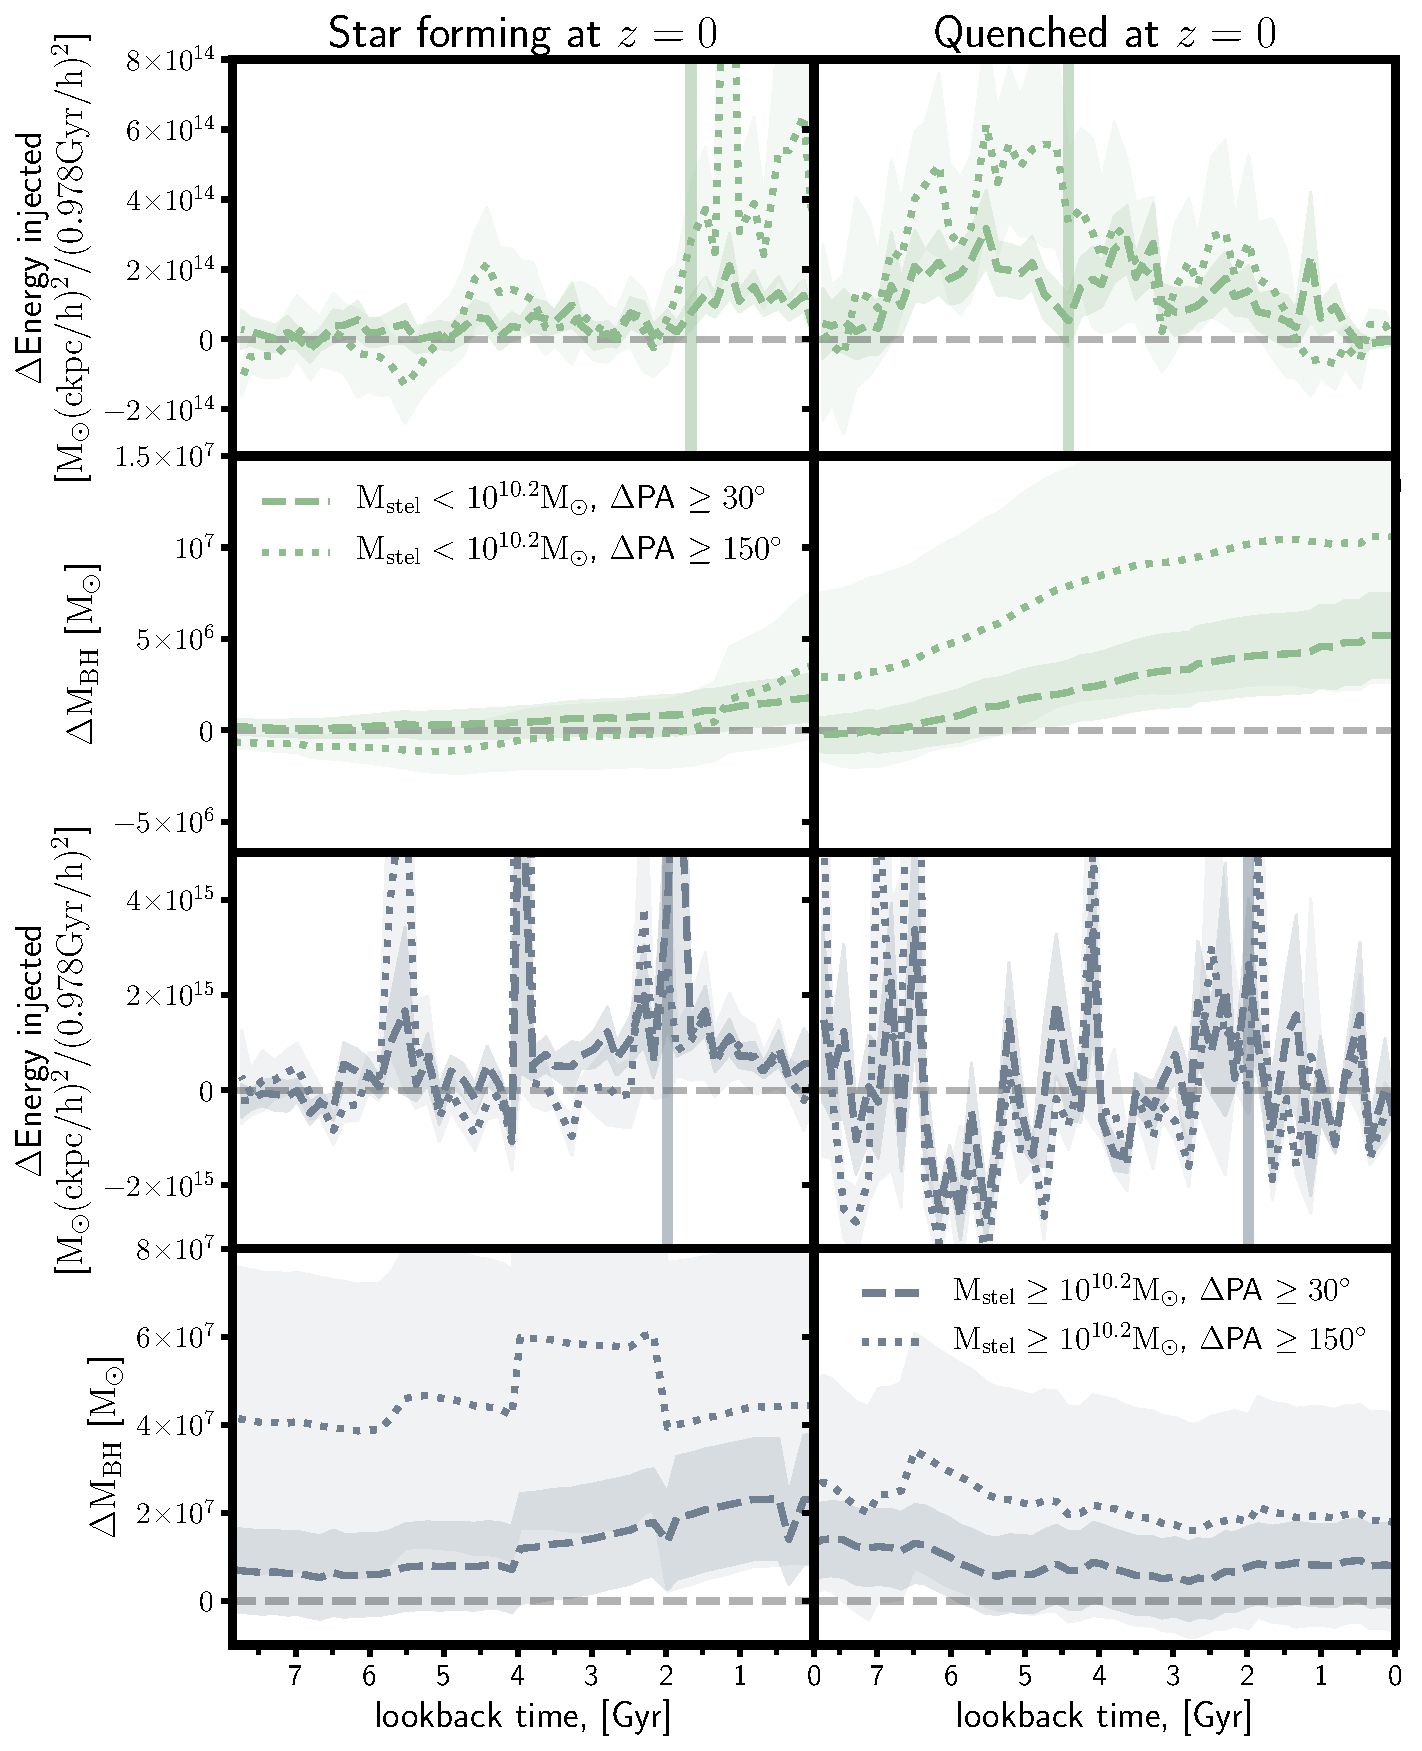
\includegraphics[width=\linewidth]{misalignment_BH/BH_props_only.pdf}
    \caption{Time evolution of black hole feedback energy injection and black hole mass for star forming (left) and quenched galaxies (right). Each row shows the residuals ($\Delta$Energy injected$\mathrm{ = E_{Misaligned/Counter-rotating} - E_{Aligned}}$) or $\Delta \mathrm{M_{BH}}$ where galaxies with $\Delta$PA $\geq 30^{\circ}$ (dashed) and $\Delta$PA $\geq 150^{\circ}$ (dotted) are defined relative to $\Delta$PA$ < 30^{\circ}$. The vertical line in the energy injection panels represents the time at which 50\% of the energy over the last 8 Gyrs has been injected. The top (bottom) two rows show the trends for low (high) mass galaxies.}
    \label{fig:BH_props}
\end{figure}

For the low mass galaxies, we find that the rate of energy injection is typically elevated for counter-rotating galaxies, however a clear boost can be seen for all those that are misaligned at $z=0$. The look-back time of peak energy injection is earlier for quenched galaxies relative to the star forming (the solid vertical line represents the time at which 50\% of the energy over the last 8 Gyrs has been injected). Misaligned star forming galaxies show far more recent feedback and BH luminosity, possibly indicative that the feedback has not fully suppressed star formation yet. Conversely, the quenched galaxies exhibit earlier peak energy injection which through this feedback suppressing star formation leads to the quenched classification at $z=0$. For this reason selecting misaligned star forming and quenched galaxies at $z=0$ will naturally lead to different time correlations in BH activity. This can be visualized by the diagram in Figure \ref{fig:diagram}. Here we depict the time evolution of a model low mass galaxy that transitions in SFR from high to low due to a radiative feedback event. At each step in the evolution we create representations of IFU observations, if made at that point in the galaxy's evolution. Due to the persistence of kinematic misalignment lasting much longer that the high AGN luminosity state, this explains the difficulty in correlating the two at a single time-step. 

\begin{landscape}
\begin{figure}
	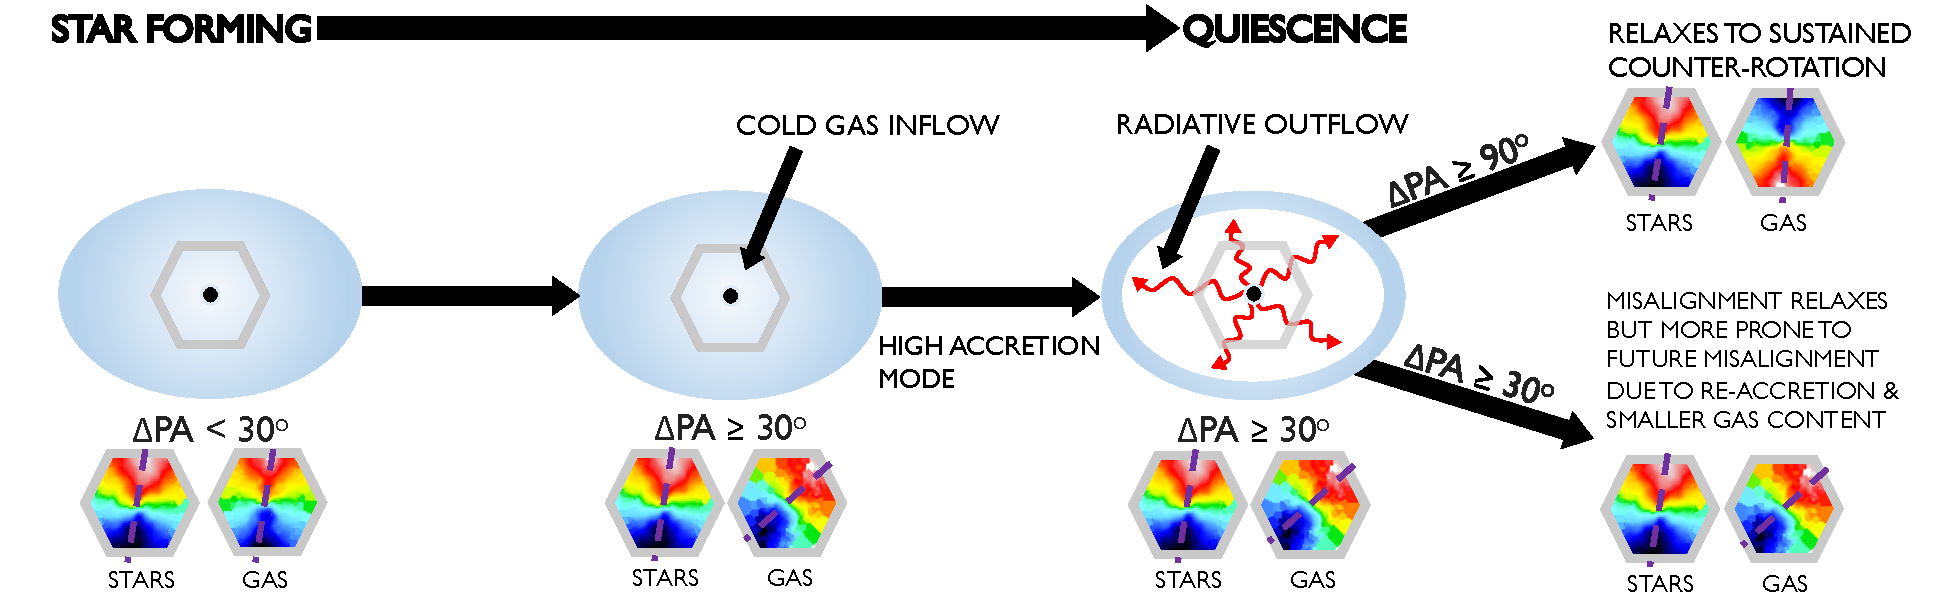
\includegraphics[width=\linewidth]{misalignment_BH/quasar_mode_feedback_compressed.pdf}
    \caption{Diagram of the relationship between BH accretion, radiative feedback, and kinematic misalignment in low mass galaxies. The diagram (left to right) shows the time evolution of radiative feedback which injects thermal energy into the cold gas reservoir of galaxy after a high accretion state triggered by a possible inflow of cold gas. Below this are representations of stellar and gas velocity fields showing what we may expect to see in an IFS observation if it was made at this time. $\Delta$PA refers to the difference between the global position angles (purple lines) for the stellar and gas velocity fields. High accretion onto the BH is directly related to boosted BH luminosity in our model. Over time radiative outflows act to suppress star formation leading to quiescence. Given that first misalignment ($\Delta$PA $\geq 30^{\circ}$) most commonly occurs around the high accretion period, we see that selecting different sSFR low mass galaxies at $z=0$ would result in different timescales since the peak AGN luminosity. Star forming galaxies with misalignment at $z=0$ will have had more recent peak energy injection since the feedback hasn't had time to fully suppress star formation yet (fifth row in Figure \ref{fig:overall_pop}).}
    \label{fig:diagram}
\end{figure}
\end{landscape}

We also show the residual time evolution of black hole mass with respect to the aligned galaxies (Figure \ref{fig:BH_props} row 2 for low mass galaxies). We find that BH growth correlates with the time scales of energy injection, indicating the close relationship between feedback and accretion for those misaligned. The causality between BH growth and feedback is however not clear. While BH growth leads to increased feedback by design, with respect to a possible correlation between feedback and the onset of misalignment the question of causality remains. One possibility is that the angular momentum is disrupted prior to feedback, potentially due to mergers. Alternatively, gas removal due to feedback could facilitate (re-)accretion of (misaligned) gas which disrupts angular momentum and then leads to increased BH growth. We again note that misaligned high mass star forming galaxies (third row, left panel) demonstrate the same qualitative trends with BH feedback and growth as the low mass, corroborating that radiative feedback is likely dominant for this sub-sample. Misaligned and counter-rotating high mass quenched galaxies show little obvious trends of BH feedback energy and growth relative to the aligned.

\subsection{Correlating kinematic misalignment and AGN at $z=0$}
To understand how kinematic misalignment may correlate with BH luminosity at $z=0$ alone, in the top panel of Figure \ref{fig:PAdist}, we show the distribution of $\Delta$PA for the top 20\% BH luminosity in our low mass sample ($\mathrm{M_{stel} < 10^{10.2}M_{\odot}}$, both the star-forming and quenched galaxies) in comparison with a control sample (all defined at $z=0$). The control is made by taking the closest unique match in stellar mass for each high BH luminosity galaxy from the remainder of our sample. We find the two distributions are statistically indistinguishable (Anderson-Darling statistic; -0.001 with a p-value of 0.348). In the bottom panel we show the same but instead we select the top 20\% in peak BH luminosity (for each galaxy in our low mass sample) over the last 8 Gyrs. In this instance the AGN bright galaxies are distinctly more misaligned than the mass matched control (Anderson-Darling statistic; 13.793 with a p-value of $3 \times 10^{-5}$). 

\begin{figure}
    \centering
	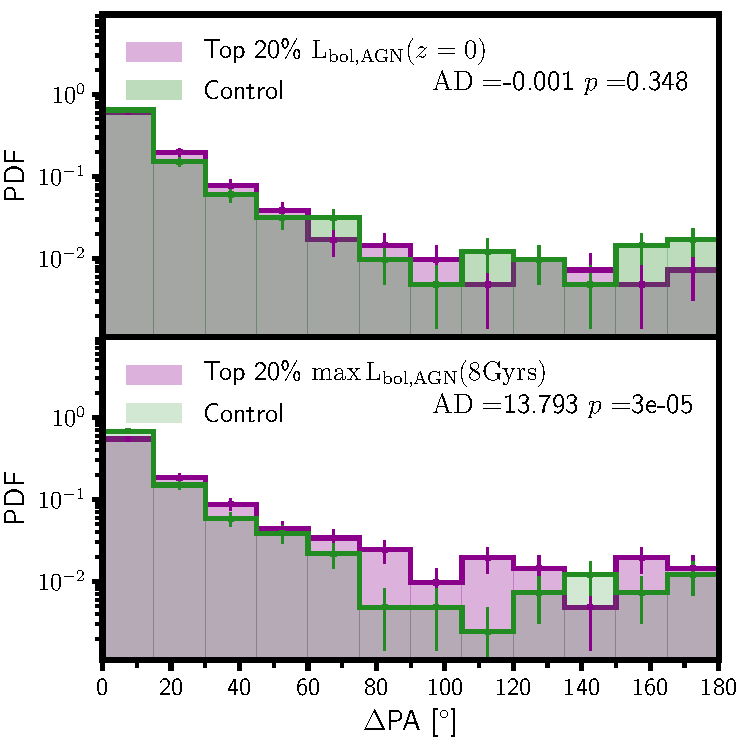
\includegraphics[width=0.9\linewidth]{misalignment_BH/PA_distribution_low_mass_z0_max_comparison.pdf}
    \caption{Probability density function of kinematic misalignment as defined by $\Delta$PA at $z=0$ for low mass galaxies ($\mathrm{M_{stel} < 10^{10.2}M_{\odot}}$). In both panels the brightest 20\% in $\mathrm{L_{bol,AGN}}$ (purple) compared with a mass matched control (green) is shown. The top panel shows the brightest in $\mathrm{L_{bol,AGN}}$ at $z=0$ only, whereas the bottom panel shows those with the brightest peak $\mathrm{L_{bol, AGN}}$ over the last 8 Gyrs. In each panel the Anderson-Darling statistic with a corresponding p-value is shown. We find no statistical difference between the active galaxies and the control for those selected at $z=0$ only, whereas we find that those which have been the most luminous over the last 8 Gyrs are distinctly more misaligned.}
    \label{fig:PAdist}
\end{figure}

This demonstrates that despite the inherent relationship between BH luminosity, feedback, and gas kinematics, considering the overall distribution of $\Delta$PA split on instantaneous luminosity at $z=0$ does not necessitate that correlation is found. This matches that of observations in MaNGA \citep[Figure 6 in][]{ilha2019}, who also find no correlation between active galaxies and a control sample. We emphasise that while our results indicate a correlation between feedback and misalignment, the decoupled rotation of gas can remain for several Gyr after initially becoming misaligned, meaning that a single epoch is unlikely to characterise the relationship for an ensemble of galaxies.

We note that IllustrisTNG typically under-produces bright AGN ($\mathrm{L_{X-ray}(2-10 keV) > 10^{44}ergs^{-1}}$) for $z \leq 1$ in contrast with observational constraints \citep[see][]{habouzit2019}. Given this and the uncertainty in estimating BH luminosity from simulations (treatment of radiatively efficient and inefficient AGN \& obscuration), we chose to select by percentile rather than cutting on absolute luminosity. Regardless, selecting only bright AGN in this way or choosing a higher percentile does not change our conclusions.

\section{Summary} \label{sec:summary_BH}
In this chapter, we study the relationship between BH luminosity, BH feedback and kinematic misalignment between stars and gas for galaxies in TNG100. We use mock observations of an IFS survey (MaNGA) built from galaxies in TNG100, to identify kinematic misalignment ($\Delta$PA; difference in PAs of stars and gas) at $z=0$. We split our mock IFS sample on stellar mass to separate the impact of `quasar' feedback from `kinetic' feedback. We follow the time evolution of BH luminosity and energy injection from BH feedback in leading up to misalignment (or counter-rotation) at $z=0$. We also compare the $z=0$ distributions of $\Delta$PA of the most luminous BHs in our sample against a control. Our conclusions are as follows.
\begin{enumerate}
    \item Low mass galaxies with misalignment (and counter-rotation) at $z=0$ typically have had boosted BH luminosity, BH growth, and significantly more energy injected into the gas over the last 8 Gyr in comparison to aligned galaxies. Gas is potentially blown out due to the AGN feedback, losing angular momentum towards $z=0$. Along with the feedback there is an increase in the fraction of cold phase gas within 2$\mathrm{R_{e}}$ (seen also for all high mass galaxies), along with an increased metallicity. These trends are seen for low mass star-forming and quenched galaxies, and high-mass star-forming galaxies split at $z=0$.
    
    \item The epoch of peak energy injection from the quasar mode feedback is different as a function of $z=0$ sSFR for misaligned low mass galaxies. This can be explained by the relationship between energy injection from feedback and galaxy quenching. Misaligned quenched galaxies have typically experienced peak energy injection from the BH at earlier times which has since acted to suppress star formation, whereas misaligned star forming galaxies exhibit more recent energy injection.

    \item Quenched high mass galaxies with misalignment (and counter-rotation) at $z=0$ typically have similar BH luminosity over the last 8 Gyr with respect to aligned galaxies and decreased gas mass is  seen within 2$\mathrm{R_{e}}$ (but not for all gas associated with the total subhalo). Gas phase metallicity is also lower with respect to aligned galaxies. This suggests that the origin of misalignment in massive quenched galaxies is more likely due to accretion of pristine gas or loss of enriched gas. 
    
    \item We find that the distributions of kinematic misalignment are statistically indistinguishable between the top 20\% in BH luminosity of low mass galaxies in our sample and a mass matched control at $z=0$. This matches observations \citep[see Figure 6 in][]{ilha2019}. Misalignment may initially occur at a similar time to the initial high accretion state (and hence peak BH luminosity), however misalignment can persist/correlate on much longer timescales. To test this we split by the top 20\% in maximum BH luminosity (for each galaxy) over the last 8 Gyrs in comparison with a control. We find that the most luminous AGN over the last 8 Gyrs are significantly more misaligned at $z=0$. This result suggests that while one may not expect correlation with misalignment when considering BH activity at $z=0$ alone, the relationship between BH luminosity and misalignment in low mass galaxies is clear. 
\end{enumerate}
While this work clearly demonstrates the correlation between BH activity and kinematic misalignment, it makes no comment on causality. Further work is required to understand what triggers the initial high accretion mode and following period of feedback for both low and high mass galaxies.
\red{expand on further work.}
\colorlet{chaptergrey}{blue!20!}
\chapter[Kinematics, the cosmic web, and halo assembly]{Kinematics as a tool to explore the role of the cosmic web and halo assembly in galaxy evolution}
\label{ch:halo_assembly}
\vspace{-5.25in}
\includegraphics[height=1.39in]{thesis/latex/misalignment_MaNGA/kin_mis_chapter_heading_grey.pdf}
\vspace{3in}

\epigraph{This chapter is partially based on Duckworth, Tojeiro, Kraljic, Sgr\'o, Wild, Weijmans, Lacerna and Drory, in MNRAS, 448, Issue 1, 2019 and Kraljic, Duckworth, Tojeiro et al. (in prep.). Here, we investigate how large scale IFS surveys can be utilized to understand the relationship between galaxy kinematics and their large-scale environment, in the context of dark matter halo assembly.}

\section{Introduction}
\red{Expand on relationship between cosmic web and galaxy properties - maybe with a focus on spin alignment? - certainly re-introduce C. Welker stuff and extended TTT. introduce MPL-6 somehow?  talk about transition from baryonic processes on small scales and transition to how this relates to large scale structure and halo assembly.}

In Chapters 2 and 3, we demonstrated how galaxy kinematics are closely related to morphological properties, baryonic processes such as AGN feedback, and the characteristics of its surrounding dark matter halo. The stellar (dark matter halo) mass of a galaxy encodes a lot of its evolution, demonstrating that \textit{local environment} (or over-density) can explain a large part of the diversity of properties we observe.

As introduced in \S\ref{sec:cosmic_web_intro}, galaxies on large scales are organised within the cosmic network of filamentary structure. Dark matter haloes and their constituent galaxies are subject to the large-scale anisotropic forces throughout their formation and evolution, in particular shaping their initial angular momentum content, before non-linear baryonic processes take hold. Their is growing evidence that the cosmic web environment of a galaxy, also plays a significant role in galaxy evolution and is, at least partially, driving their morphology. 

Revisiting tidal torque theory \citep[TTT; e.g.][]{hoyle1951, peebles1969} in the context of large-scale anisotropic environment, \citet{codis2015} explain the relative angular momentum distribution of haloes with respect to neighbouring filaments and walls. The misalignment between the inertia tensors of the proto-haloes and the directionality of the tidal tensor due to the neighbouring wall or filament leads to a spin alignment for low mass haloes. As these haloes grow in mass hierarchically, merging with other haloes and they lose this preferential alignment with large scale structure. Due to the flow of matter along walls and filaments, mergers often happen in this plane, leading to \textit{flip} in direction, so that higher mass dark matter haloes are preferentially perpendicular to the orientation of the tidal field \citep[e.g.][]{Codis2012, dubois2014, GaneshaiahVeena2018}. This is, of course, motivated from cosmological N-body simulations and understanding how this propagates to observations is complex. In simulations, the constituent galaxies appear to retain a memory of the spin orientation (with respect to large scale structure) as dictated by their host dark matter halo \citep[e.g.][]{codis2018, Kraljic2019flip}. The mass dependence of the spin alignment \textit{flip} is, however, debated and likely dependent on different choices for baryonic processes and the scale of the neighbouring filamentary structure.

\red{add figure of spin orientation with disperse overlay?}

Historically, exploring the relationship between the spin direction of galaxies and large scale structure has been difficult. Without spatially resolved spectra of galaxies, we are reliant on projected shapes which introduces degeneracies with respect to the actual spin vector direction \citep[e.g. see Fig 2. in][for example of degeneracies that can occur]{motloch2020}. Due to this, and the different approaches to re-constructing the cosmic web, studies are often conflicting in findings \citep[e.g. spiral galaxies having parallel vs perpendicular orientations with respect to the cosmic web][]{tempel2013a, tempel2013, lee2007, jones2010, zhang2015}. These differences due to the reconstruction of the cosmic web can likely be explained due a difference in chosen scales. In hydrodynamical simulations, the transition mass from preferential parallel alignment to perpendicular alignment is very much dependent on the scale of the filamentary structure, such as width \citep{ganeshaiahveena2019, Kraljic2019flip}. Averaging over an ensemble of filamentary scales will likely wash out this transition, and hence preferential alignment in either direction. 

The other half of the problem can be solved, however, by having kinematic information for a large population of galaxies. Kinematic (rotational) position angles help break the degeneracy of shape orientation, and provide more robust measures of directionality. We are now in the era of multiple IFS surveys that may observe enough galaxies to find a significant detection of spin alignment. In section \S\ref{sec:spin_alignment}, we explore spin alignment in MaNGA for spirals and S0 galaxies.

The orientation of galaxies with respect to large-scale structure is, however, one aspect to determining the relationship between galaxy evolution and the cosmic web. As introduced in \S\ref{sec:halo_assembly_bias_intro}, the large-scale tidal forces created by the cosmic web are motivated to modulate the assembly history of dark matter haloes and their constituent galaxies, once the effect of mass has been taken into account. 

In parallel with detecting spin alignment, tracing the impact of dark matter halo assembly on galaxy observables in the local Universe is a difficult prospect. A powerful approach is to consider the wealth of spatially resolved information from surveys such as MaNGA and SAMI to deconvolve the role of differences in halo assembly history. In \S\ref{sec:halo_assembly}, we investigate if kinematically misaligned central galaxies assemble their mass differently, and are in preferentially different locations in the cosmic web.

\section{Spin alignment of spiral and S0 galaxies in MaNGA} \label{sec:spin_alignment}
\red{talk about C. Welker and Krowleski papers.}

\subsection{Data and Methods}

\subsubsection{Galaxy sample}
Throughout this chapter, we base our analysis on 4633 unique galaxy observations corresponding to the 6th MaNGA product launch (MPL). This reflects the completion of the survey as of mid-2018 (data released publicly December 2018). For each galaxy we compute kinematic position angles for both the stellar and ionized gas velocity fields. We calculate position angles as described in \S\ref{sec:kin_mis}. In this section concerning spin alignment we only make use of position angles derived from stellar kinematics, however, in \S\ref{sec:halo_assembly} we make use of the full kinematic misalignment measures. 

To compute the spin direction of each galaxy in our sample, we assume a thin disk approximation and therefore require each galaxy to have a disk component. We select our sample based on the visual morphological classifications of GalaxyZoo2 \citep[GZ2][]{willett2013} as introduced in \S\ref{sec:morph_def_obs}. We select a \textit{pure} spiral galaxy sample by taking all objects that have a debiased vote fraction of $\geq 0.9$ for answers positive to the galaxy having a disk. \red{add in lenticular definition}.

\subsubsection{DisPerSE}
For all work in this chapter, we characterise the topological features of the cosmic web using the Discrete Persistent Structure Extractor Code \citep{sousbie2011a, sousbie2011b} as introduced in \S\ref{sec:cosmic_web_intro}. Here DisPerSE is applied to a modified version of the SDSS DR10 spectroscopic sample as described in \citet{tempel2014}. In observations there is an additional difficulty since we are not working with exact three dimensional positions in real space, however, in redshift space. To recover the intrinsic galaxy position, an estimation for the peculiar velocity must be made for each galaxy. On large-scales this corresponds to the Kaiser effect \citep{kaiser1987}, which acts to increase the contrast of the skeleton due the coherent motion of galaxies with the growth of structure \citep[e.g.][]{shi2016}. On small-scales, however, the Fingers of God effect \citep[FOG;][]{jackson1972,tulley1978} derives from random motions of galaxies within virialized haloes. The latter can elongate structure in redshift space leading to erroneous identification of filaments. We correct for the FOG effect using the technique outlined in \citet{kraljic2018}. As introduced in \S\ref{sec:cosmic_web_intro}, the \textit{robustness} of the morphological features identified are quantified using the so called persistence ratio, a measure of the significance of the topological connection between individual pairs of critical points. Here we use filaments identified with a significance of 5$\sigma$ corresponding to robust structure.

The local geometry of each filament is characterised by a series of smaller \textit{segments}, which are the default output of the DisPerSE code. For each galaxy, the nearest segment is found and its direction is used to compare to the given galaxy's spin direction.
\red{find out maximum distance at which a galaxy is considered to be connected with a filament in Kat's sample.}

\subsubsection{Angular momentum directions}
In order to estimate the spin direction of our galaxy sample, we assume a thin-disk approximation according to \citet{LeeErdogdu2007}. Here we summarise the key steps in calculating the three dimensional vector. Working in spherical coordinates in the reference frame of the galaxy, the spin direction can be described as
\begin{equation}
\begin{split}
\mathrm{\hat{L}_r & = \cos i,} \\
\mathrm{\hat{L}_{\theta} & = (1 - \cos^2 i)^{1/2} \sin PA,} \\
\mathrm{\hat{L}_{\phi} & = (1 - \cos^2 i)^{1/2} \cos PA,}
\end{split}    
\end{equation}
where $\mathrm{PA}$ is the position angle from the stellar kinematics and $i$ is the inclination of the galaxy, defined as such
\begin{equation}
\mathrm{\cos^2 i = \frac{(b/a)^2 - p^2}{1 - p^2},}
\end{equation}
where $b/a$ is the sky projected axis ratio and $p$ is the intrinsic flatness of the galaxy \citep[varies as a function of morphology as described in][]{haynes1984}. $p$ accounts for the fact that the disk of galaxies has a finite thickness, and the presence of a bulge impacts the estimation of $b/a$. In this work we adopt an intermediate value (0.158), however choosing more extreme proposed values (0.1 - 0.23) does not change our findings. The value of $i$ is set to $\pi/2$ if $b/a < p$.

The spin direction can then be transformed into equatorial Cartesian coordinates as follows:
\begin{equation}
\begin{split}
    \hat{L}_x & = \hat{L}_r \sin \alpha \cos \beta + \hat{L}_{\theta} \cos \alpha \cos \beta - \hat{L}_{\phi} \sin \beta \\
    \hat{L}_y & = \hat{L}_r \sin \alpha \sin \beta + \hat{L}_{\theta} \cos \alpha \sin \beta + \hat{L}_{\phi} \cos \beta \\
    \hat{L}_z & = \hat{L}_r \cos \alpha - \hat{L}_{\theta} \sin \alpha
\end{split}    
\end{equation}
where $\alpha = \pi/2 - {\rm dec}$ and $\beta = {\rm RA}$.

% %We apply positive sign to $\hat{L}_r$ to all galaxies 
% %It is worth mentioning here that the spin vector determined from equation (9) suffers from the sign ambiguity in Lr, as mentioned in Pen et al. (2000) and Trujillo et al. (2006). Since it is not possible to determine the sign of Lr from the given information of the Tully Catalog, we apply positive sign to all Tully galaxies here. We expect that this sign ambiguity will play a role in decreasing the strength of the spin-shear alignment signal.
% \Kat{Talk about the ambiguity in the sign of $\hat{L}_r$ and the adopted positive value. Maybe we could do better, Chris I think you should have an information on whether it is positive of negative, no?}

\subsection{Spin alignment}
\subsubsection{LTGs}
\begin{figure}
    \centering
    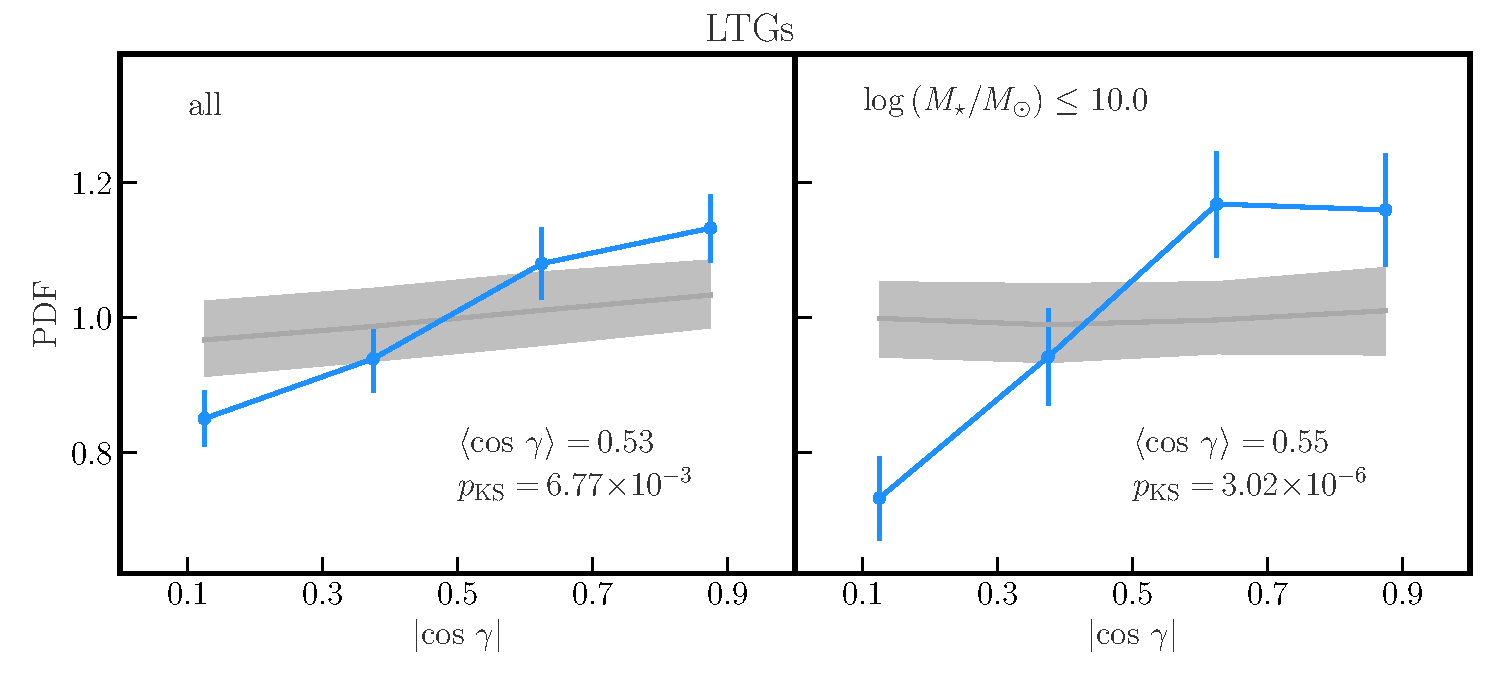
\includegraphics[width=\linewidth]{thesis/latex/halo_assembly_manga/spin_fil_LTGs_2in1.pdf}
    \caption{Alignment between neighbouring filament and spin direction of late type galaxies calculated from the thin disk approximation. Each panel shows the probability density distribution (blue) of the cosine angle between the direction of the filament segment and the spin direction. Errors are calculated through bootstrapping and the grey line (with associated errors) corresponds to the expected distribution for a completely random alignment. In addition, each panel shows the mean $\cos \gamma$ for the population and the $p$-value for a Kolmogorov--Smirnov test. The left panel shows for all LTGs in our sample, whereas the right panel shows the distribution only for those with a stellar mass $< 10^{10} M_{\odot}$. We find that for all masses LTGs are preferentially \textit{parallel} orientated with respect to the neighbouring filament, with low mass showing a more significant alignment signal.}
    \label{fig:ltgs_spin_alignment} 
\end{figure}

In Figure \ref{fig:ltgs_spin_alignment}, we show the probability density function of alignment between the spin directions of LTGs and their neighbouring filament segment. We define $\gamma$ as the angle between the spin direction and segment directions. The PDF is presented as $|\cos \gamma|$ so that 0 corresponds to exact perpendicular alignment and 1 exact parallel alignment. Each panel shows the distribution for LTGs (blue) with associated bootstrap errors, along with the expectation of the distribution if the spin vectors have completely random orientations (grey line with errors). In addition, each panel shows the mean $\cos \gamma$ for the population and the $p$-value for a Kolmogorov--Smirnov (KS) test between the LTGs and the random orientations. A KS test evaluates if two sub-populations are drawn from the same distribution with the null hypothesis that they are consistent. A low $p$-value therefore signifies that the populations are independent to the significance level stated. 

In the left panel, we show the orientations for all LTGs selected in our sample. We find that the spin of LTGs are preferentially orientated \textit{parallel} to the direction of the neighbouring filament segment, to the significance level of $p_{KS} = 6.77 x 10^{-3}$. In the right panel, we show the PDF for only LTGs that are below a stellar mass of $\mathrm{M_{stel} < 10^{10} M_{\odot}}$. Again we find a preferential parallel alignment, however, now to an increased significance level of $p_{KS} = 3.02 x 10^{-6}$. In addition $\langle \cos \gamma \rangle$ increases from 0.53 (all LTGs) to 0.55 (low mass LTGs), indicative that this signal is strongest for the low mass LTGs. This parallel alignment is in-keeping with theoretical expectation that the formation of low mass disks tend to align with the large-scale tidal field in which they evolve. 

\subsubsection{S0s}
\begin{figure}
    \centering
    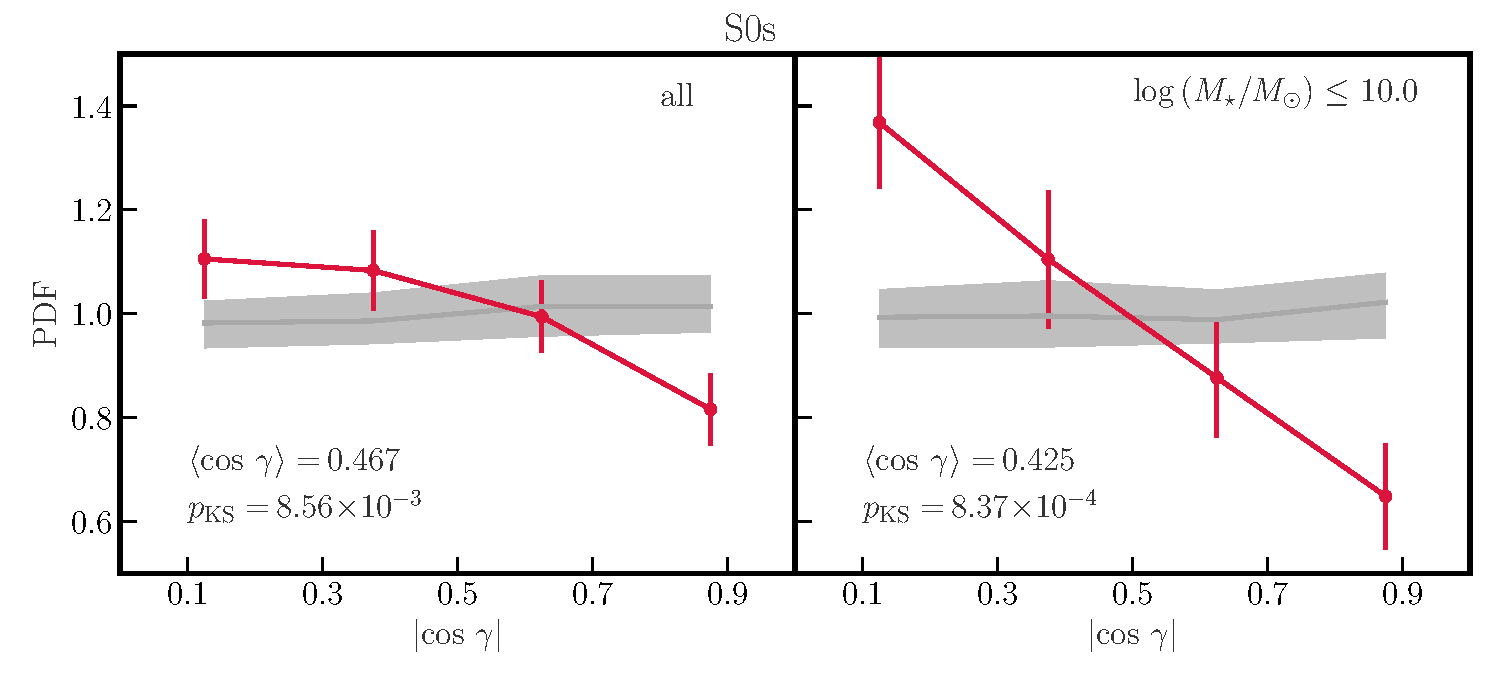
\includegraphics[width=\linewidth]{thesis/latex/halo_assembly_manga/spin_fil_S0s_2in1.pdf}
    \caption{Alignment between neighbouring filament and spin direction of lenticular galaxies calculated from the thin disk approximation. Each panel shows the probability density distribution (red) of the cosine angle between the direction of the filament segment and the spin direction. Errors are calculated through bootstrapping and the grey line (with associated errors) corresponds to the expected distribution for a completely random alignment. In addition, each panel shows the mean $\cos \gamma$ for the population and the $p$-value for a Kolmogorov--Smirnov test. The left panel shows for all S0s in our sample, whereas the right panel shows the distribution only for those with a stellar mass $< 10^{10} M_{stel}$. We find that for all masses lenticulars are preferentially \textit{perpendicular} orientated with respect to the neighbouring filament, with low mass showing a more significant alignment signal.}
    \label{fig:s0_spin_alignment}
\end{figure}

In Figure \ref{fig:s0_spin_alignment}, we now show the PDF of alignment between the disks of lenticular galaxies and their neighbouring filament segment. As before, we show the PDF as a $\cos \gamma$ distribution with the left panel showing the results for all S0s in our sample and the right for low mass ($\mathrm{M_{stel} < 10^{10} M_{\odot}}$) S0s only. Here, we find that the spin direction of S0s are preferentially \textit{perpendicular} with respect to their neighbouring filament segment. Considering the null hypothesis that the spin directions have random orientation, we find that the total S0 population is different from random to a significance of $p_{KS} = 8.56 x 10^{-3}$ which increases to  $p_{KS} = 8.37 x 10^{-4}$ when only considering the low mass S0s. This preferential perpendicular alignment could be indicative of the evolutionary history of lenticular galaxies embedded in large filamentary structure. The expectation from N-body simulations is that the orientation of dark matter haloes flip in direction due to mergers in the plane of the filament. This could be indicative that the S0s near filamentary structure have undergone mergers in their recent history, leading to a perpendicular orientation. 

\subsection{Discussion and Summary}
Of most relevance to our findings are the studies of spin alignment which also make use of large scale IFS surveys. In the SAMI survey, \citet{welker2020} correlate the spin directions of galaxies estimated from kinematics with the direction of the nearest filament segment (also defined using DisPerSE). They find evidence that low mass galaxies are preferentially parallel to filaments, whereas high mass galaxies are preferentially perpendicular (to a significance of 2$\sigma$). This is in agreement with expectations of a spin \textit{flip} seen for dark matter haloes in N-body simulations, due to initial preferential alignment (for low mass haloes) with the tidal field, before mergers in the plane of the filament cause a flip in orientation. Conversely in MaNGA \citet{krolewski2019} find no evidence for spin alignment with neighbouring cosmic web structure using the vector computed from stellar velocity fields. 

In both studies the spin alignment signal is computed using the spin and filament vectors in projected 2D space. While this reduces uncertainty when reconstructing the 3D spin vector (i.e. such as making an assumption of a thin disk approximation), it does not make use of the 3D information associated with filament reconstruction. Additionally making use of only the 2D information enables studies of galaxies without disks. Projecting the angle between two 3D vectors into 2D introduces possible projection degeneracies (see black histogram in Figure \ref{fig:PA_residual}) corresponding to a standard deviation of $\sim 13^{\circ}$ from the intrinsic value.

Our work represents the first study using IFS data to estimate 3D spin directions and correlating them with neighbouring filamentary structure. Our key findings are as follows: 
\begin{itemize}
    \item Spiral galaxies demonstrate preferentially \textit{parallel} spin orientations with respect to the nearest filament segment. The significance of the alignment signal is increased if we only consider low mass LTGs ($\mathrm{M_{stel} < 10^{10} M_{\odot}}$). 
    \item Lenticular galaxies demonstrate preferentially \textit{perpendicular} spin orientations with respect to the nearest filament segment. The significance of the alignment signal is increased if we only consider low mass S0s ($\mathrm{M_{stel} < 10^{10} M_{\odot}}$). 
\end{itemize}

Parallel spin alignment between LTGs and filaments is in agreement with \cite{welker2020} and expectations from N-body simulations \citep[e.g.][]{laigle2015}. Our finding of perpendicular alignment for lenticulars, especially for those low mass, is perhaps more surprising. This is in direct conflict with the expectation that low mass galaxies have a parallel orientation, which flips as they grow in mass. This could be indicative that the orientation is not only a function of mass, \textit{but also of morphology.} Following the idea that lenticulars form through mergers, this could be indicative of a spin \textit{flip} at lower masses as the galaxy becomes re-orientated which is reflected in the galaxy morphology. In the next section, we make further use of MaNGA to explore the connection between the cosmic web and galaxy kinematics, \textit{now} in the context of halo assembly.

\section{Kinematically misaligned galaxies and halo assembly} \label{sec:halo_assembly}
In this section, the kinematic misalignment, $\Delta$PA, of central galaxies will be correlated with various environment dependent parameters for the surrounding halo. Following the discussion of \citet{hahn2009}, the current accretion rate is correlated with the large-scale tidal environment. Low-mass haloes in the vicinity of large haloes or massive structures will have their accretion `stalled' as tidal forces overcome their ability to accrete \citep[see also;][]{wang2007,dalal2008,lacerna2011}. Accordingly, this would lead to a relatively earlier formation time and a lack of on-going accretion seen today. Conversely low-mass haloes in environments of low magnitude tidal forces will continue accreting, and could have a late halo assembly time and continued gas accretion onto the central galaxy today. 
% We explore whether position with respect to filamentary structures identified in the cosmic web, halo age and estimated group occupancy correlate with more recent accretion observed on the central galaxy of the group. A younger halo corresponds, by definition, to more recent dark matter accretion and a richer recent merger history. We explore the idea that low-mass haloes have their cold flow accretion halted due to large-scale tidal environment as indicated by the halo age or vicinity to cosmic web features. 

\subsection{Estimators of halo assembly and environment}
In this section we explore these ideas with the following tests:
\begin{enumerate}
\item Cosmic web classification (Section \ref{sec:cw_classification_hab})
\begin{itemize}
\item Distances of haloes to filamentary structures are considered for galaxies split on $\Delta$PA. We test if low-mass haloes near filaments have their accretion `stalled' due to material preferentially flowing along the filament to more dense regions. 
\end{itemize}
\item Stellar to halo mass ratio  (Section \ref{sec:MsMh_hab})
\begin{itemize}
\item The stellar to halo mass ratio is used as a proxy for halo age and its correlation with $\Delta$PA is considered. We test if large-scale tidal forces can `stall' accretion onto low-mass haloes, seen as a low accretion rate today ($\Delta$PA < 30$^{\circ}$) on the central galaxy, indicating an earlier forming halo.
\end{itemize}
\item HOD modelling (Section \ref{sec:HOD_hab})
\begin{itemize}
\item A halo occupation distribution is constructed for groups with aligned and misaligned central galaxies. Earlier forming haloes provide more time for centrals to form and satellites to merge. This would correspond to a decrease in the magnitude of the HOD, which we aim to isolate. 
\end{itemize}
\end{enumerate}
In each section we present both our method and results. The impact of environment on kinematically misaligned galaxies has been previously studied in MaNGA. Using a sample of 66 misaligned galaxies, \citet{jin2016} found that the fraction of misalignment varies with galaxy properties such as stellar mass and sSFR. Regardless of sSFR, they find that kinematically misaligned galaxies are typically more isolated. Could these correspond to the later forming haloes?

\subsection{Data}
\red{Here, we describe the additional data used and our sample selection for this section.}

\subsubsection{Stellar mass and halo mass definitions} \label{sec:mass_hab}
We use stellar masses estimated in the New-York University Value Added Catalogue from the K-correct routine \citep[NYU-VAC;][]{blanton2005}. To analyse the incident effects onto central galaxies as a function of environment, we require both group identification and estimations of the total halo mass. \citet{yang2007} (Y07 hence-forth) present an adaptive group finding algorithm based on the NYU-VAC to assign galaxies to haloes and then estimate and revise group properties through iteration. We will summarise the basic steps here. Potential group centres are first found through a friend-of-friends algorithm with small linking lengths in redshift space. All galaxies not currently linked are also considered as potential centres. For each tentative group, the combined luminosity of all group members with 
\begin{equation}
^{0.1}M_r - 5log(h) \leq -19.5
\end{equation}
are found, where $^{0.1}M_r$ is the absolute magnitude estimated from the NYU-VAC K-corrected to $z=0.1$. All galaxies within SDSS data-release 7 (DR7, all spectroscopic galaxies) below $z=0.09$ meet this criteria and hence the combined luminosity can be estimated directly. A corrective factor is applied for groups above this redshift. This total luminosity is then used to assign halo mass and various other group properties, which in turn refines the group identification following an iterative process until conversion. 

We remove all groups with $f_{edge} < 0.6$ as recommended by Y07 corresponding to groups on the survey borders. \citet{yang2009} provide a conservative estimate on the minimum halo mass for groups that would be expected to be complete as a function of redshift. This work primarily focusses on low-mass haloes, ($M_h \lesssim 10^{12.5} M_{\odot}$), however many of these groups will be incomplete at the redshift range selected. Y07 note however that any potential scatter arising from the incompleteness correction should be minimal in comparison with the scatter between group luminosity and assigned halo mass. 

The use of a group catalogue brings important considerations. In low-mass groups, the multiplicity of each group is low, and the luminosity (or stellar mass) of the central galaxy, will largely determine the mass of the group, potentially leading to an under-estimation of the scatter in the stellar-mass to halo-mass relation (see e.g. \citealt{campbell2015, reddick2013}). On the other hand, the fraction of groups with at least one satellite galaxy that is more massive than the central, increases steeply with halo mass (see e.g. \citealt{reddick2013}), leading to artificially larger scatter and an increased likelihood of central misclassification with increasing halo mass. \citet{campbell2015} demonstrate that group finder inferred measurements tend to equalise the properties of distinct galaxy sub-populations, however in general it is possible to recover meaningful physical correlations for average properties as a function of stellar and halo mass. 

We select only galaxies classified as centrals corresponding to the most massive galaxy within each group identified by Y07. The relationship between the central stellar mass and halo mass for galaxies within Y07 is shown in Figure \ref{fig:stel_halo_dist}. The increase of scatter in this relationship with increasing halo mass is likely explained by the limitations of group catalogues mentioned above. 

\begin{figure}
    \centering
	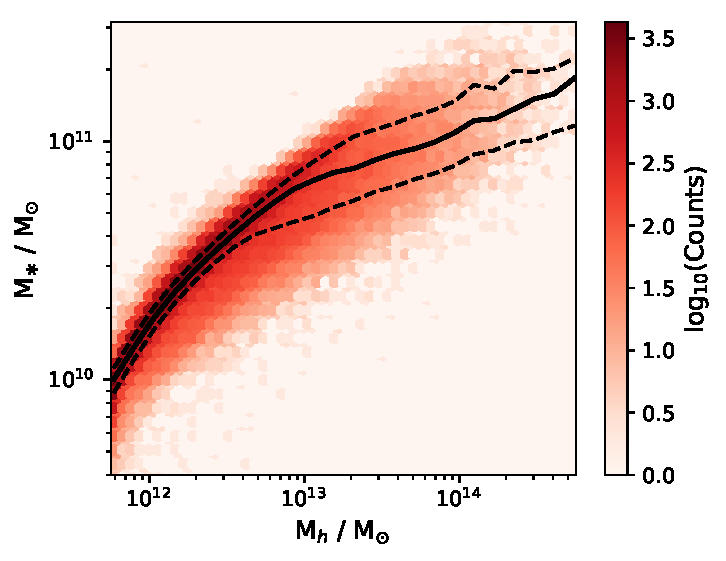
\includegraphics[width=0.8\linewidth]{thesis/latex/misalignment_MaNGA/stel_halo_ratio_dist.pdf}
    \caption[Hexagonal density plot of the relationship between the stellar mass  and the halo mass for central galaxies within Y07]{Hexagonal density plot of the relationship between the stellar mass  and the halo mass for central galaxies within Y07. The number counts are scaled logarithmically. The black lines show the median (solid) and the 20th and 80th quantiles (dashed) of the stellar mass in bins of halo mass.}
    \label{fig:stel_halo_dist}
\end{figure}

\subsubsection{Sample selection} \label{sec:samp_sec}
While the complete MaNGA sample may be unbiased to morphology, we must proceed with care when selecting a sub-sample usable for kinematic disturbance. To remove spurious PA fits we eyeball the entire MPL-6 sample and remove all galaxies which have a largely incomplete velocity field, poor or biased PA fit or are virtually face-on so that little or no rotational component is along the line of sight. This removes approximately half of MPL-6 observations. The majority of galaxies removed have largely incomplete gas velocity fields and for that reason our analysis naturally excludes gas-poor and slowly rotating elliptical galaxies. 

Recent studies have found that the fraction of slow rotators increases steeply with stellar mass and has a weak dependence on environment once this is controlled for \citep[e.g.][]{greene2018,lagos2018}. We note that our natural exclusion of gas-poor high-mass galaxies is reflected in the stellar mass distribution of the $\Delta$PA defined sample in Figure \ref{fig:samp_cons}. \red{Reference NSA target catalogue?}

\begin{figure}
    \centering
	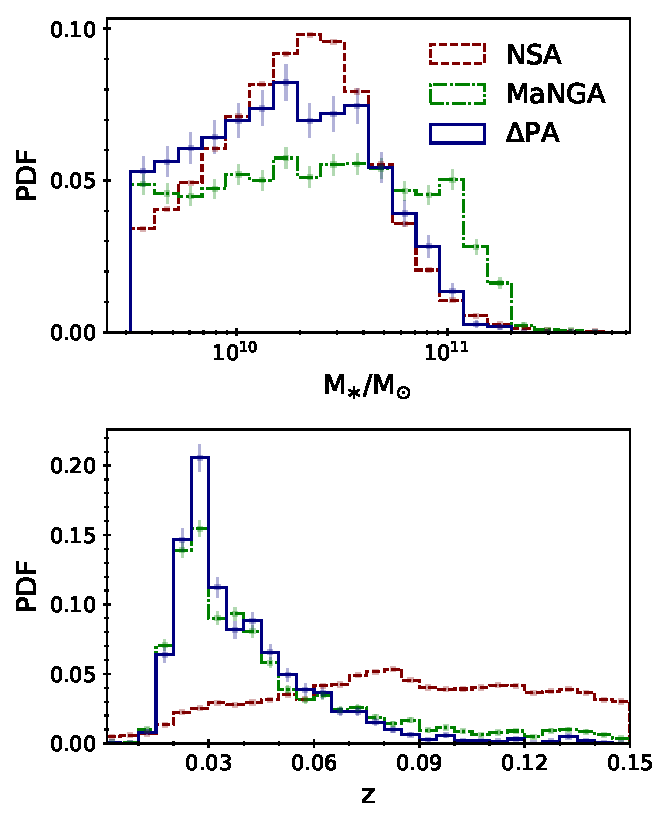
\includegraphics[width=0.6\linewidth]{thesis/latex/halo_assembly_manga/sample_consistency.pdf}
    \caption[Relative frequency distributions of stellar mass and redshift for the NSA target catalogue, MaNGA MPL-6 and $\Delta$PA sub-samples.]{Relative frequency distributions of stellar mass and redshift for the NSA target catalogue (brown dashed line), MaNGA MPL-6 (green dot-dashed line) and our $\Delta$PA sub-sample (blue solid line). The figure is cut at $z=0.15$ representing the extent of MaNGA targets. Each histogram is given with Poisson errors on each bin.}
    \label{fig:samp_cons}
\end{figure}

GalaxyZoo1\footnote{At the point of submission for this work, GalaxyZoo1 provided the largest sample of galaxies with classified morphologies for the MaNGA survey. Since then a complete catalogue for all MaNGA targets has been constructed which will be used and described in \red{Chapter...}} provides visually identified morphologies for a large sample of SDSS galaxies \citep{lintott2008}. Morphology is identified by having over 80\% of debiased classification votes in the same category (i.e. elliptical or spiral). The remainder of galaxies are marked as uncertain morphology. We compare the fraction of ellipticals in our $\Delta$PA sub-sample with MPL-6, as shown in Table \ref{tab:GZ}. GalaxyZoo1 only provides classifications for 3/4 of MPL-6 as reflected by the total classification numbers. We find the fraction of ETGs falls from 0.242 to 0.111, reaffirming our bias against slow-rotating high-mass ellipticals that our eye-balling tends to remove. 

If galaxies are truly morphologically transformed, then this should be reflected in their angular momentum. \citet{cortese2016} find that galaxies lie on a tight plane defined by stellar angular momentum ($j_{stars}$), S\'ersic index and stellar mass when excluding slow rotators in the SAMI galaxy Survey. This could indicate that fast rotating early-type and late-type galaxies are not two distinct populations but instead represent a continuum connecting pure-discs to bulge dominated systems \citep{cappellari2011}. This can be linked to simulation: \citet{lagos2017} use EAGLE \citep{EAGLE2015} to investigate the effects of galaxy mergers on the evolution of stellar specific angular momentum. They find that the gas content of a merger is the most important factor for dictating $j_{stars}$ for the remnant, ahead of both the mass ratio and spin/orbital orientation of the merger progenitors. An increasing rate of wet (gas-rich) mergers corresponds to decreasing stellar mass and increasing $j_{stars}$. Conversely dry (gas-poor) mergers are the most effective way of spinning down galaxies, with gas-poor counter-rotating progenitors creating the biggest decrease in $j_{stars}$. Following this narrative, it is fair to exclude slow rotators which could follow a different evolutionary track to a continuum of fast rotating galaxies in angular momentum phase space. 

\red{We note that the initial GalaxyZoo1 classifications mirror our findings in Section X. Despite the $\Delta$PA defined galaxies in this analysis being predominately classified as LTGs, we find the majority of kinematically misaligned galaxies are ETGs. The ubiquity of misalignment in ETGs and lack there-of in LTGs is a distinct question which is covered in more depth in Chapter X.} 

%The ubiquity of misalignment in ETGs and lack there-of in LTGs is however a distinct question which could be explained by the relative relaxation time-scales of galaxies of different intrinsic angular momenta or the fractions of in-situ/ex-situ origin of gas. This could, however, be a natural result of disc formation and sustainment arising from cold flows of the cosmic web \citep{pichon2011}. If the disc is preferentially aligned with its larger surrounding structure then further directional accretion would be unlikely to create a kinematic misalignment. The low fraction of kinematically misaligned blue galaxies was first noted by \citet{chen2016} who explored a possible mechanism for their formation and characteristics. Selecting only early-type galaxies and comparing the misaligned sub-sample with a stellar mass weighted control does not fundamentally change any of the results presented here. While understanding how a morphology bias could impact any results presented, we leave its origin the focus of future work. 

\begin{table}
\centering
\begin{tabular}{|l|c|c|c|c|}
\hline
& Total & GZ1 & ETG & LTG \\ \hline
MPL-6 & 4614 & 3598 & 869 (0.242) & 1225 (0.340) \\
$\Delta$PA defined & 2272 & 1835 & 204 (0.111) & 1005 (0.548) \\
$\Delta$PA > 30$^{\circ}$ & 192 & 151 & 85 (0.556) & 9 (0.060)\\
Final sample & 925 & 812 & 136 (0.167) & 456 (0.561) \\ \hline
\end{tabular}
\caption{(Rows: top to bottom) All usable MPL-6 galaxies, all $\Delta$PA defined galaxies within MPL-6, those that are kinematically misaligned with $\Delta$PA > 30$^{\circ}$ and the final sample of central, $\Delta$PA defined galaxies used in this Chapter. For each row, the total number of galaxies is given, along with those defined in GalaxyZoo1 (denoted GZ1 in table) and the total number of which that are classified into early-type (ETG) and late-type (LTG). The fractions of early-types and late-types are defined with respect to the total number of GalaxyZoo1 defined galaxies.}
\label{tab:GZ}
\end{table}

We are looking for accretion due to large-scale influence, so we remove all obvious on-going mergers through visual inspection of both the field photometry and IFU observations. We also identify target galaxies interacting with close pairs or neighbours. While this visual inspection should identify the majority of on-going major mergers, we note that our identifications are clearly subjective. We remove $\sim$50 galaxies, identified to be merging or interacting with a nearby neighbour. After matching to the Y07 group catalogue for halo mass we are left with 925 central galaxies which we use in this chapter. 

\subsection{Cosmic web classification} \label{sec:cw_classification_hab}
We explore the ability of a low-mass halo to accrete with respect to where it falls within the cosmic web. 
% \citet{ZOMGI} find that low mass halos within large filaments typically correspond to this `stalled' scenario. Dark matter and baryonic material flows along the filament towards high density nodes (intersection of filaments), which starves the low mass halo residing between nodes (however accretion may be allowed to continue perpendicular to the filament - should still be a lower rate today). Conversely low mass halos residing at the convergence point of multiple small filaments correspond to environments of low tidal force strength as isotropic accretion is allowed to continue. This test correlates distances to various cosmic web features with $\Delta$PA.
To characterise topological features, such as the filaments which could lead to the suppression of accretion, the Discrete Persistent Structure Extractor code \citep[DisPerSE;][]{sousbie2011a,sousbie2011b} is applied to a modified SDSS DR10 spectroscopic catalogue \citep{tempel2014}. 
% \citet{kraljic2018} applied DisPerSE to GAMA and analysed various galaxy properties such as u-r colour, specific star formation rate (sSFR) and stellar mass relative to distances to different cosmic web features. They find significant mass and colour gradients with more massive and passive galaxies typically residing closer to both filaments and the points of their intersection (nodes). For fixed stellar mass, the star forming population appears to redden with decreasing distance to filaments \blue{plot?}. This trend can be seen well outside the virial radii of the galaxies and underlying structure and hence can be considered as `pre-processing' which can be explained by large scale filamentary tides rather than any density effect. This can be interpreted as anisotropic assembly bias, that at fixed mass the accretion rate varies with the orientation and distance to filaments. 

\subsection{DisPerSE}

\red{refer to section in introduction?}

% DisPerSE is a geometric three-dimensional ridge extractor that applies directly to point-like distributions, making it particularly well adapted for astrophysical applications, as demonstrated by its previous application to various large galaxy surveys, such as SDSS \citep{sousbie2011b}, GAMA \citep{kraljic2018} or VIPERS \citep{malavasi2017}. 

% It is based on discrete Morse and persistence theories, allowing for a scale and parameter-free coherent identification of the 3D structures of the cosmic web as dictated by the large-scale topology. 

% In a nutshell, discrete homology is used to build the so-called Morse-Smale complex on the point-like tracers. This geometrical segmentation of space defines distinct regions called ascending manifolds that are identified as individual morphological components of the cosmic web; i.e. ascending manifolds of dimension 3, 2, 1 and 0 as voids, walls, filaments and nodes of the cosmic web, respectively. 

% In addition to its ability to work with sparsely sampled data sets and assuming nothing about the geometry or homogeneity of the survey, retained structures can be selected on the basis of their significance compared to shot noise. DisPerSE hence allows to trace precisely the locus of filaments, walls and voids using the so called persistence ratio, a measure of the significance of the topological connection between individual pairs of critical points, mimicking thus an adaptive smoothing depending on the local level of noise. In practice, this threshold is expressed in term of number of $\sigma$.

% In this work, DisPerSE is run with a 5$\sigma$ persistence threshold to extract the persistent cosmic web from the density field as computed from the discrete distribution of the galaxies in the SDSS main sample using the Delaunay Tessellation Field Estimator technique (DTFE; \citet{schaap2000}; \citet{cautun2011}). An illustration of the filamentary network overlaid with the density contrast of the underlying galaxy distribution for the SDSS field is shown in Figure \ref{fig:disperse_sdss}. 

% Being reliant on the three-dimensional distribution of galaxies, DisPerSE is therefore affected by redshift space distortions. On large-scales this corresponds to the Kaiser effect \citep{kaiser1987}, which acts to increase the contrast of the skeleton due the coherent motion of galaxies with the growth of structure \citep[e.g.][]{shi2016}. On small-scales, however, the Fingers of God effect \citep[FOG;][]{jackson1972,tulley1978} derives from random motions of galaxies within virialized haloes. The latter can elongate structure in redshift space leading to erroneous identification of filaments. We correct for the FOG effect using the technique outlined in \citet{kraljic2018}.

\subsubsection{Cosmic web distances}
Having constructed a skeleton of the cosmic web, a galaxy's environment can be described by finding its vicinity to various features of the skeleton. The cosmic web comprises of low density `void' regions which are enclosed by `walls' of structure which become filaments at points of intersection. The gravitational potential of the filaments dictate the flow of the matter, which at the point of intersection, feed high density regions interpreted as `nodes'. Along the filament, saddle points remain as minima between the flows towards nodes.  
% GAMA has a completeness of > 98\% down to a r-band apparent magnitude of $m_r$ = 19.8 whereas... Care must therefore be taken when making any direct comparisons between GAMA and DR7.

The distance to the nearest filamentary point, $D_{skel}$, is first found for each galaxy. To then consider the influence of the nearest node, the distance from this impact point along the filament to the node is also computed, $D_{node}$. Finally the distance to the nearest wall, $D_{wall}$, can then be found. In order to investigate expected trends of galaxies with vicinity to any cosmic web feature we must remove effects resulting due to the proximity of others. For $D_{skel}$ we remove all galaxies that lie within $D_{node} < 0.5$ Mpc. 
% and for $D_{wall}$, all galaxies within $D_{node} < 0.5$ Mpc and $D_{skel} < 2.5$ Mpc are discounted. 
This represents a compromise between eliminating the effect of other cosmic web features and having enough galaxies left to construct a statistically significant sample. Tightening the condition with respect to nodes so that we require $D_{node} > 1$ Mpc does not change any of the results presented in this work. 
We do not include analysis with respect to the walls since we limited to low numbers after removing galaxies that could be influenced by nodes and/or filaments.

Construction of the cosmic web from any observation is influenced by the completeness and the sampling of the galaxy sample. The modified SDSS DR10 spectroscopic sample is complete to $m_r$ = 17.77. A sample containing only brighter galaxies will naturally only identify stronger/larger filamentary features and hence smaller substructures will be missed. In addition, the lower the sampling of galaxies, the lesser the accuracy of the actual position of cosmic web features. To correct for this, the distances are normalised by the mean inter-galaxy separation, $\left\langle D_z \right\rangle$ at a given redshift, as such $\left\langle D_z \right\rangle = n(z)^{-1/3}$ where $n(z)$ is the number density. 

\subsubsection{Environmental density and stellar mass}
Before we consider the role of the cosmic web, we consider the role of environmental density and stellar mass in our results. A dependence on small scale density is an indirect effect of halo mass and would not probe the large-scale anisotropy of the cosmic web. It is also important to isolate the role of stellar mass and morphology following their distinct gradients with respect to cosmic web features found in GAMA \citep{kraljic2018}.

Figure \ref{fig:density_hab} shows the distributions of densities and stellar mass for the aligned and misaligned samples. Density used in this work is computed using a Delaunay tessellation of the discrete galaxy positions through the DTFE estimator, smoothed with a Gaussian kernel at local scales (3 Mpc) and at large scales (9 Mpc). 

We evaluate the likelihood of the aligned and misaligned sample being drawn from the same continuous distribution through implementation of a two-sample Kolmogorov--Smirnov (KS) test. In each case a D-value of the KS statistic with a corresponding p-value is provided. The D-value (referred to as the KS statistic hence-forth) provides the maximum fractional difference between the cumulative distribution functions with a p-value corresponding to the null hypothesis that the two samples are drawn from the same continuous distribution. A high KS value combined with a low p-value (for example; KS $\geq$ 0.1 for P $\leq$ 10\% confidence level) therefore is consistent with the two samples being significantly different.

The first row of Figure \ref{fig:density_hab} considers the difference between all $\Delta$PA defined galaxies. We find that the misaligned galaxies ($\Delta$PA > 30$^{\circ}$) reside in more dense environments at small and large scales with a probability that the distributions are instead consistent of 0.3\% and 0.5\% respectively. The two samples are consistent in distribution of stellar mass, despite the difference in classified morphology, as shown in Table \ref{tab:GZ}. In the second row of Figure \ref{fig:density_hab} we consider the same properties but only for ETGs. We select on optical morphology using the classifications of GalaxyZoo1 as introduced in \S\ref{sec:samp_sec}. We find that the difference seen in density smoothed on small scales may be explained by morphology as the p-value for the KS test increases, however misaligned galaxies tend to reside in more dense large-scale environments and populate lower stellar masses compared with aligned galaxies of the same morphology.

In order to minimize the effect of $\rho_{3Mpc}$ and $M_{\ast}$ in our cosmic web results, in the next section we weight distance distributions on both stellar mass and small scale density, when comparing the distribution of cosmic distances for the aligned and misaligned samples. This is done through normalising the histogram of the weight quantity to be consistent between distributions using a minimum of three bins. We also include the results of ETGs only to minimize the impact of morphology. We cannot do the same for LTGs due to the lack of misaligned LTGs. 

\begin{figure*}
    \centering
	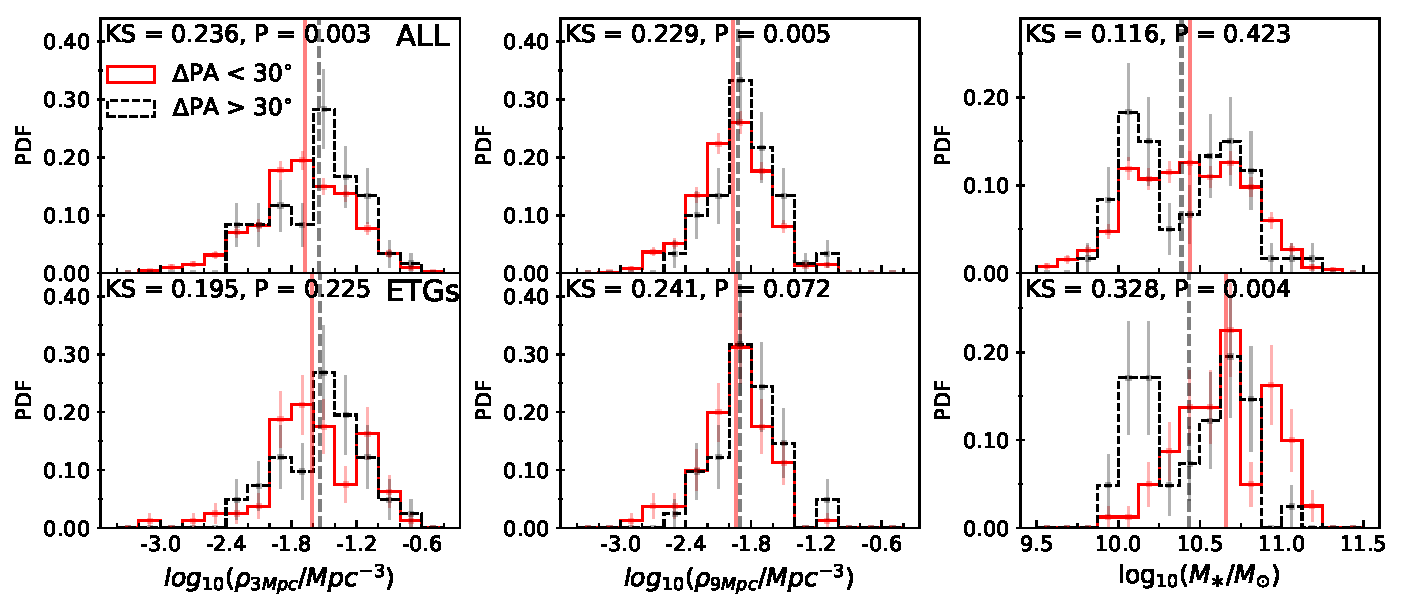
\includegraphics[width=\linewidth]{thesis/latex/halo_assembly_manga/PA_ALL_ET_DENSITY.pdf}
    \caption[Probability density distributions of density smoothed with a Gaussian kernel at the scale of 3 Mpc \& 9 Mpc and the stellar mass, log$_{10}(M_{\ast}/M_{\odot})$ for all $\Delta$PA defined galaxies and all GalaxyZoo1 classified elliptical galaxies with a $\Delta$PA.]{Probability density distributions of density smoothed with a Gaussian kernel at the scale of 3 Mpc \& 9 Mpc and the stellar mass, log$_{10}(M_{\ast}/M_{\odot})$ (left to right) for all $\Delta$PA defined galaxies (top row) and all GalaxyZoo1 classified elliptical galaxies with a $\Delta$PA (bottom row). Aligned galaxies ($\Delta$PA < 30$^{\circ}$) are shown in red (solid line) and those with high misalignment ($\Delta$PA > 30$^{\circ}$) are in black (dashed line). Each histogram is given with Poisson errors on each bin. A two-sample KS statistic and its corresponding p-value is overlaid for comparison between the distributions in each cell and the vertical lines denote the corresponding distribution's median. Using all galaxies, the misaligned sample resides in higher density at the scales of 3 Mpc and 9 Mpc to the aligned sample respectively, but are equivalent in stellar mass. Selecting only ETGs accounts for the difference in small scale density but the misaligned sample are at lower stellar masses than the aligned.}
    \label{fig:density_hab}
\end{figure*}

\subsubsection{Results of cosmic web distances} \label{sec:cw_res}
Figure \ref{fig:cw_all} shows the distance probability density distributions of aligned and misaligned galaxies with respect to nodes (left) and filaments (right). The top row shows the two samples weighted on stellar mass, the middle row weighted on small scale density (3 Mpc smoothed) and the bottom row shows the raw distributions. The results of a two-sample KS test with corresponding weightings to the cumulative distribution function are overlaid in each cell. 
% This is to assess if any signal is an indirect result of halo mass, rather than the tidal forces we aim to probe. 

%We do not include interpretation of the distribution of misaligned galaxies with respect to walls since we are limited to very low numbers and they are left unweighted. 
The distributions of aligned and misaligned galaxies with respect to filaments meet the null hypothesis criterion of high p-values for all weighting schemes (i.e. no statistically significant difference between distributions). This is indicative that $\Delta$PA is independent of the influence of filaments identified in our analysis. For the unweighted samples, we find that misaligned galaxies typically reside in closer vicinity to nodes than their aligned counterparts as indicated by a p-value of 0.089. This difference is however partially negated by weighting on stellar mass or density smoothed on the 3 Mpc scale, as reflected in slightly reduced KS values and p-values increased above the 0.1 significance level.

The origin of misaligned galaxies residing preferentially closer to nodes could be explained by their morphology difference with respect to the aligned sample. In previous work, \citet{kraljic2018} found distinct gradients of stellar mass and morphology with vicinity to nodes and filaments. Figure \ref{fig:cw_et} shows the distributions of cosmic web feature distances but now only selecting ETGs. We find that in all weighting schemes, the distance distributions of aligned and misaligned galaxies with respect to both nodes and filaments meet the null hypothesis criterion as reflected in large p-values (> 0.4). These distributions appear to be drawn from the same continuous distribution, indicating that direct and indirect effects of morphology are likely responsible for the difference in distance to nodes. 
% In all cases we find no statistical difference between distances to features for the aligned and misaligned galaxies. As previously noted, GalaxyZoo1 only provides classifications for 3/4 of MPL-6. 

\begin{figure}
    \centering
	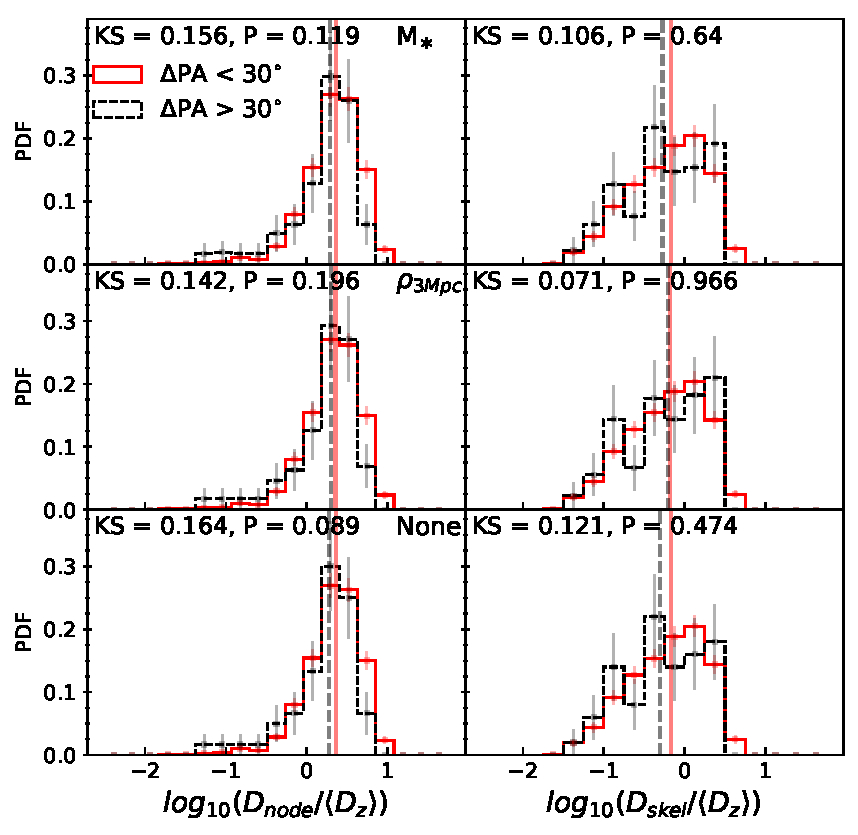
\includegraphics[width=0.85\linewidth]{thesis/latex/halo_assembly_manga/PA_ALL_CW.pdf}
    \caption[Probability density distributions of normalised distances to cosmic web features for all $\Delta$PA defined galaxies.]{Probability density distributions of normalised distances to cosmic web features for all $\Delta$PA defined galaxies. Distances to nodes (left) and filaments (right) are normalised by the sampling at a given redshift. The distributions of galaxies in the top row is weighted on stellar mass between the aligned (red solid line) and misaligned samples (black dashed line). The distributions are weighted by density smoothed by a Gaussian kernel at the scale of 3 Mpc for the middle row and are left unweighted for the bottom row. A two-sample KS statistic and its corresponding p-value is overlaid for comparison between the distributions in each cell. The error bars represent the poisson noise in each bin. The weighted median values for each distribution are shown by the vertical lines.}
    \label{fig:cw_all}
\end{figure}

\begin{figure}
    \centering
	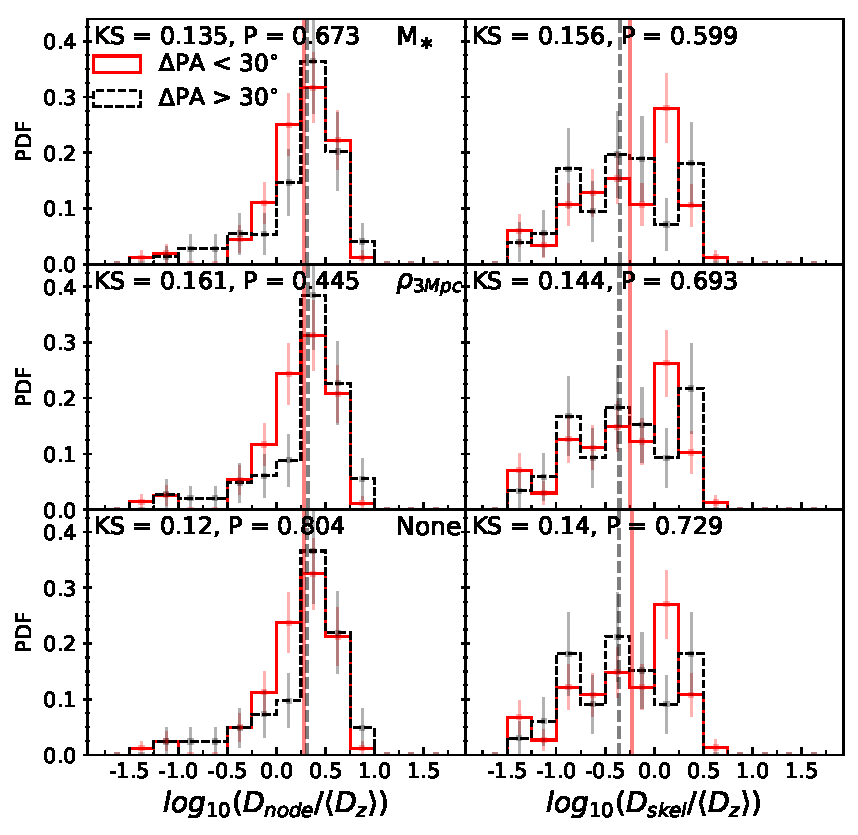
\includegraphics[width=0.9\linewidth]{thesis/latex/halo_assembly_manga/PA_ET_CW.pdf}
    \caption{Same as Figure \ref{fig:cw_all} but using only visually selected ETGs as found in GalaxyZoo1.}
    \label{fig:cw_et}
\end{figure}

\subsubsection{The role of halo mass} 
Our primary aim in this section is to isolate if vicinity to filaments can impact the rate of present-time accretion on a central galaxy in a low-mass halo. Including high-mass haloes in our sample may counteract any observable signal as they are possible candidates responsible for quenching accretion. High-mass, typically old haloes, are the opposite of what we are trying to target: young, still forming low-mass haloes (with respect to old low-mass haloes). 

We now consider $D_{skel}$ for low-mass haloes only. \citet{tojeiro2017} found signal of halo assembly bias in low-mass haloes using the stellar to halo mass ratio in GAMA. Low-mass haloes residing in regions of stronger tidal forces were found to form earlier irrespective of density, with this trend apparently reversed at high mass. This signal was found to be strongest for haloes of mass $M_h \sim 10^{12.3} M_{\odot}$, however a slight trend was found even at $M_h \sim 10^{12.74} M_{\odot}$. To ensure we have enough objects for a statistically significant sample we therefore consider all central galaxies residing in haloes of mass: $M_h \sim 10^{12.5} M_{\odot}$. Figure \ref{fig:mh_cw} shows the distance probability density distributions for the whole $\Delta$PA defined sample and GalaxyZoo1 defined ETGs only. For all weighting schemes, we find p-values consistently above the 0.1 significance level and hence conclude the null hypothesis that the aligned and misaligned galaxies are consistent in distance distributions with respect to filaments. This holds true regardless of morphology selection.

\begin{figure}
	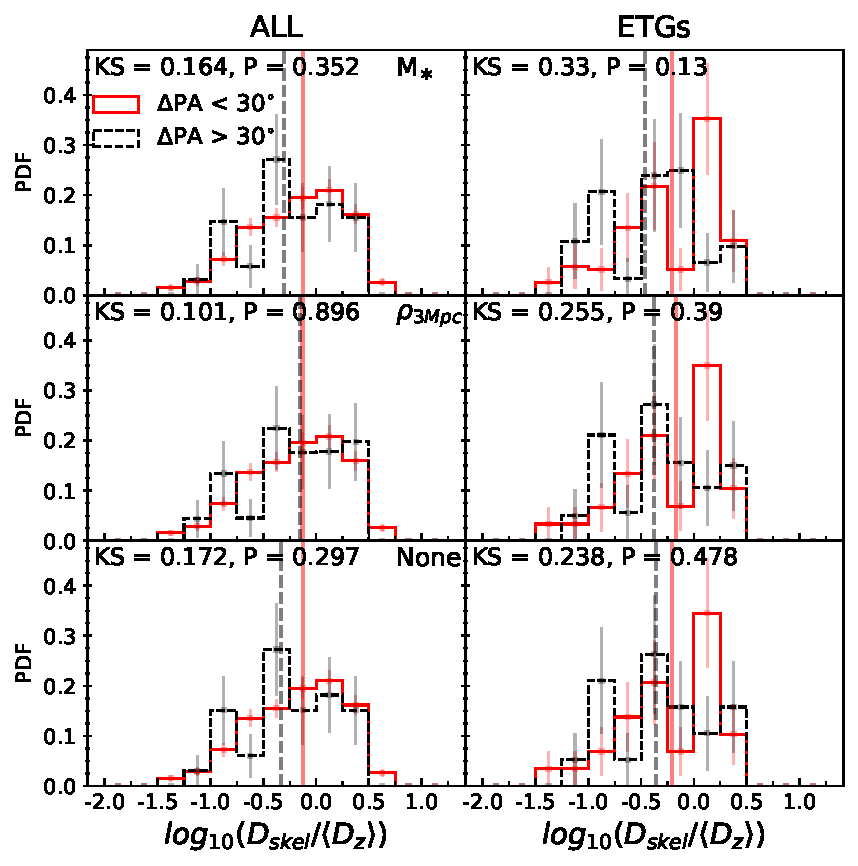
\includegraphics[width=\linewidth]{thesis/latex/halo_assembly_manga/PA_ALL_CW_Mh12_5.pdf}
    \caption[Probability density distributions of normalised distances to filaments for galaxies in MaNGA MPL-6.]{Probability density distributions of normalised distances to filaments for galaxies with log$_{10}$(M$_h$/M$_{\odot}) \le 12.5$. As in Figure \ref{fig:cw_all} the distributions are weighted on stellar mass (top), density smoothed at scales of 3 Mpc (middle) and left unweighted (bottom). The distributions of all $\Delta$PA defined galaxies (left) and only galaxyZoo selected ETGs (right) are shown for comparison.}
    \label{fig:mh_cw}
\end{figure}

\subsection{Stellar to halo mass ratio}\label{sec:MsMh_hab}
In this section we introduce an observational proxy for halo formation time: the central stellar to total halo mass ratio. Its use was motivated in \citet{wang2011} who explored the correlation between various halo properties which were identified within a set of seven N-body simulations using the P\textsuperscript{3}M code described in \citet{jing2007}. One of the most important properties is its formation time, $z_f$ which was shown to correlate with galaxy properties such as SFR, galaxy age and colour. The formation time in this instance is defined as the redshift at which the main progenitor has formed half of the mass of the final halo. %An observational counterpart must be constructed as $z_f$ cannot be determined from galaxies alone. 
They establish that formation time shows a tight correlation with the sub-structure fraction, $f_s = 1 - M_{main}/M_h$, where $M_{main}$ and $M_h$ are the main \textit{sub}-halo mass and the halo mass respectively \citep{gao2007}. 
The ratio of $M_{main}$ and the total halo mass is seen to act as an robust estimate for formation time. Following \citet{lim2015}, we use the following as an observational proxy,
\begin{equation}
f_c = \frac{M_{*,c}}{M_h},
\end{equation}
where $M_{*,c}$ is the stellar mass of the central galaxy. The $M_h$ in this instance is found using the group stellar mass ranking from Y07. $M_{*,c}$ is a reasonable estimator for the main sub-halo mass $M_{main}$ however they do not hold an exactly monotonic relation. Given this and that $f_s$ is not perfectly correlated with formation time, $f_c$ can only be considered to be a relative proxy of $z_f$ as shown in \citet{lim2015}. A higher value of $M_{*,c}/M_h$ should correspond to a relatively older halo. 
Semi-analytic and hydrodynamical simulations have since confirmed a correlation between halo assembly time and the stellar to halo mass ratio, and have shown how halo formation time partly explains the scatter in the stellar mass to halo mass relation \citep[e.g.][]{matthee2017,tojeiro2017,zehavi2018}. Observationally, \cite{tojeiro2017} show that the stellar to halo mass ratio of central galaxies varied with position within the cosmic web, at fixed halo mass. In this section, we investigate whether recent accretion history, associated with younger halos, might be visible in the kinematics of gas and stars.

\subsubsection{Results of the halo age proxy}
Figure \ref{fig:2d_ratio} shows the stellar to halo mass ratio as function of $\Delta$PA. Since we do not possess errors for stellar mass or halo mass and can only roughly estimate $\Delta$PA errors, we bin our data and calculate the standard error on the mean. We split our sample at the median halo mass of $M_{\ast} = 10^{12.3} M_{\odot}$ and divide galaxies into bins with boundaries; $\Delta$PA$ = [0,5,10,20,90,180] (^{\circ})$. In each of the halo mass bins, we weigh the redshift and halo mass distributions to be consistent in each bin of $\Delta$PA. Figure \ref{fig:2d_ratio} shows no particular dependence on $\Delta$PA for this proxy of halo age. However, given the strong dependence of $M_{\ast}/M_{h}$ on $M_{h}$, we investigate this further by simultaneously considering the relationship between $M_{h}$, $M_{\ast}/M_{h}$ and $\Delta$PA. 

\begin{figure}
    \centering
	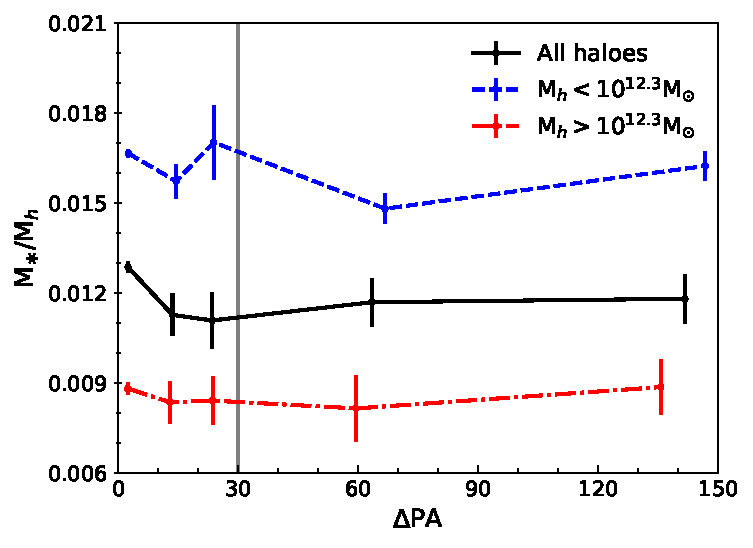
\includegraphics[width=0.8\linewidth]{thesis/latex/halo_assembly_manga/stel_halo_ratio_bin0_10_20_30_90.pdf}
    \caption[The central stellar to total halo mass ratio for the $\Delta$PA sub-sample.]{The central stellar to total halo mass ratio for the $\Delta$PA sub-sample in bins of halo mass. Galaxies residing in haloes of M$_{\ast} < 10^{12.3}$M$_{\odot}$ (blue dashed line), M$_{\ast} > 10^{12.3}$M$_{\odot}$ (red dot-dashed line) and the total sample (black solid line) are divided into bins of $\Delta$PA$ = [0,10,20,30,90,180] (^{\circ})$. Error-bars are given by the standard error on the mean. Within each bin of halo mass, distributions are weighted on redshift and halo mass between all $\Delta$PA bins.}
    \label{fig:2d_ratio}
\end{figure}

%Figure \ref{fig:plane_fit} shows the three parameter space. 
We divide our parameter space into quarters by splitting galaxies at $\Delta$PA = 30$^{\circ}$ and $M_{h} = 10^{12.3}M_{\odot}$. In each region we fit a flat plane to our data points as described by,
\begin{equation}
M_{\ast}/M_{h} = c_{0} log_{10}(M_{h}/M_{\odot}) + c_{1}\Delta PA + c_{2}.
\end{equation}
A strong correlation between $M_{\ast}/M_{h}$ and $\Delta$PA would correspond to a relatively large value of $c_{1}$ with regards to $c_{0}$. To understand the significance of any result, we also fit a flat plane with $c_{1} = 0$ (i.e. no dependence on $\Delta$PA) and evaluate $\chi_{red}^2$ for both. These values are found in Table \ref{tab:chisq}. We are inherently limited by having no errors on the estimates of stellar mass and halo mass for our sample. We therefore construct constant errors across the sample estimated from the sample variance. The sample variance itself is found from considering each data point with regards to its 10 nearest neighbours in the parameter space. 

We find that fixing the gradient along $\Delta$PA has little or no effect on the fit of the linear plane, regardless of how we sub-divide our parameter space. In some cases the comparison planes are effectively the same allowing for a smaller $\chi_{red}^2$ for the two free parameter fit. As discussed in \S\ref{sec:mass_hab}, halo masses assigned to galaxy groups using the Y07 group catalogue are corrected due to incompleteness above $z=0.09$. We consider the plane fitting again but with redshift cuts at both $z=0.09$ and a conservative $z=0.05$. In both instances, we also find there are no statistically significant gradients along $\Delta$PA. We therefore conclude that $\Delta$PA holds little correlation with the age of the halo in which it resides, as inferred from current measurements of $M_{\ast}/M_{h}$. 

% \begin{figure}
% 	\includegraphics[width=\linewidth]{stel_halo_param_chisq_fit}
%     \caption{Parameter space for the central stellar to halo mass ratio (M$_{\ast}$/M$_{h}$), halo mass (M$_{h}$) and $\Delta$PA. $\Delta$PA and M$_{h}$ are scaled logarithmically for presentation purposes. All scatter points correspond to galaxies within our analysis and are fit by 2D planes through least squares minimization. Each colour corresponds to the parameter space range in which a plane was fitted. The parameter space is divided at $\Delta$PA = 30$^{\circ}$ corresponding to red and black filled colours below and above this. It is secondly split at $M_{h} = 10^{12.3}M_{\odot}$ with blue and red edge colours corresponding to low and high mass respectively.}
%     \label{fig:plane_fit}
% \end{figure}

\begin{table}
\centering
\begin{tabular}{|l|c|c|c|}
\hline
$M_{h}/M_{\odot}$& & $\Delta$PA = [0, 30]($^{\circ}$) & $\Delta$PA = [30, 180]($^{\circ}$) \\ \hline 
[$10^{11.7}, 10^{12.3}$] & $c_{1} = 0$: & 1.188 & 1.070 \\
					   & Free : & 1.190 & 1.068 \\ \hline
[$10^{12.3}, 10^{14}$]   & $c_{1} = 0$: & 1.218 & 0.988 \\ 
					   & Free: & 1.212 & 1.001 \\ \hline
% fix units on this table
\end{tabular}
\caption{$\chi_{red}^2$ for plane fits with $c_1 = 0$ and left free in the parameter space for the central stellar to halo mass ratio (M$_{\ast}$/M$_{h}$), halo mass (M$_{h}$) and $\Delta$PA. The parameter space is divided at $\Delta$PA = 30$^{\circ}$ and $M_{h} = 10^{12.3}M_{\odot}$.}
\label{tab:chisq}
\end{table}

\subsection{Halo occupation distribution} \label{sec:HOD_hab}
In this section we introduce the HOD function and how it can be used to infer halo age. In describing the relationship between galaxies and dark matter haloes, HODs are a useful prescription to determine models of galaxy formation and evolution \citep[e.g.][]{berlind2003}. They provide a probability distribution function $P(N|M_h)$ for a set of virialised haloes where $N$ is the number of hosted galaxies for a given halo mass $M_h$. A fundamental assumption underlying HOD modelling is that the galaxy occupation is purely dependent on the halo mass. Typically the observed galaxy clustering is used to construct the empirical relationship that allows mock dark matter haloes to be populated with galaxies. Assembly bias would directly affect the observed clustering of galaxies and hence challenge any interpretation using the HOD framework. 

Continuing our discussion, low-mass haloes near large haloes are expected to cease formation earlier. This leads to a boost of galaxy clustering at this halo mass range relative to the overall sample as they live preferentially in high density regions. \citet{zehavi2018} previously investigated the dependence of occupation functions on various properties such as large-scale environmental density and halo age using semi-analytical galaxy models applied to the Millennium simulation \citep{springel2005} \citep[See also;][who confirmed these results using the hydro simulations of EAGLE and Illustris]{artale2018}. They find that higher density environments generally act to populate lower mass haloes with central galaxies. A stronger dependence can be found on halo age, however, as earlier forming low-mass haloes are more likely to host central galaxies. In addition, earlier forming haloes are likely to host fewer satellites relative to late forming haloes at fixed halo mass. A simple explanation is that the early forming haloes provide more time for their constituent satellite galaxies to merge with the central. More massive central galaxies may therefore reside in low-mass haloes that formed early due to this general in-flow, analogous to a higher stellar to halo mass ratio. 

\subsubsection{Background subtraction}
To understand the assembly history of a central galaxy's sub-halo we must consider the role of satellites that contribute to the hierarchical structure growth of its halo merger tree. However, we are limited by the magnitude and typical size of galaxies inhibiting small substructure around a main sub-halo. \citet{liu2011} demonstrate a common method for counter-acting the lack of spectroscopic information for satellite galaxies through counting possible photometric group members. Their numbers are then statistically corrected to remove the contribution of contaminant foreground and background galaxies outside of the group. This enables a lower limit of apparent magnitudes which can be accessed through use of the background subtraction technique. \citet{rodriguez2015} extend this formalism to HOD modelling and provide the technique we implement here. For a complete description of the technique we direct the reader to this reference, however we will summarise the basic concepts here.

Background subtraction requires two catalogues that share the same sky area; we will use our $\Delta$PA defined MaNGA centrals with their identified groups in combination with the photometric SDSS catalogue. For the photometric galaxies in the sky region of a group, their absolute magnitudes are calculated at the redshift of the group, $z_{f}$. The total number of galaxies with an absolute magnitude $M \le M_{min}$ are then counted within a circle around the group centre with its radius determined by the projected characteristic radius on the sky. In order to remove background galaxies, an estimation of the local density with respect to the average catalogue density must be made. All galaxies with $M \le M_{min}$ are recounted in concentric annuli centred on the group to provide the local density. A correction for the total number of galaxies in the group can then be estimated by subtracting the local background density multiplied by the group's projected area. The HOD is then constructed by binning the groups into mass intervals and averaging.

\citet{rodriguez2015} demonstrate the recovery of the background subtraction method using mock catalogues constructed from semi-analytic models of galaxy formation applied on top of the Millennium simulation. They compare the HODs found from the background subtraction technique to HODs of the direct galaxy counts in volume limited samples for different magnitude limits \citep[see Figure 1 in;][]{rodriguez2015}. Beyond a small overprediction for fainter magnitudes ($M_{lim} \approx -16.0$), they find good agreement with direct galaxy counts for all absolute magnitudes.

Results from the background subtraction technique have also been compared to results of other HOD estimation techniques applied to observations. \citet{yang2008} parametrise HODs for satellite galaxies in groups identified in SDSS DR4 using the adaptive group-finding algorithm of Y07 (see \S\ref{sec:mass_hab} for discussion). The background subtraction technique shows great agreement in estimating parameters of the HOD relative to the method of \citet{yang2008} but additionally offers the ability to estimate the HOD for fainter absolute magnitudes than previous work \citep[see Figure 5 in][]{rodriguez2015}.

MPL-6 does not provide a large enough sample size to construct a reliable two-halo term in HOD modelling through calculation of the cross-correlation function. Background subtraction therefore represents the best estimation for this sample size.

\subsubsection{Results of the HOD}
We match each central galaxy in our $\Delta$PA sample with its corresponding satellite group members using \citet{yang2007}. We split our groups at $\Delta$PA = 10$^{\circ}$ for the central and calculate the HOD using the background subtraction technique. Our lower split in $\Delta$PA is purely due to limitations of sample numbers. As demonstrated in \S \ref{sec:kin_mis}, this should be above the resolution limit of $\Delta$PA, however may include more galaxies with spurious kinematic misalignments or due to an internal origin. 

Figure \ref{fig:hod_mpl6} shows the HOD for different magnitude cuts of the group during comparison to the photometric background. As fainter galaxies are removed, the overall magnitude of the HOD naturally decreases as we have less complete groups. As a sanity check, we compare our HODs estimated from the background subtraction technique to HODs estimated directly from clustering in SDSS DR7 with similar magnitude cuts \citep{zehavi2011}. The authors use measurements of the projected correlation function for SDSS DR7, which is translated into a HOD through use of a smoothed step function \citep[see equation 7;][]{zehavi2011}. This comparison is shown in panels II-IV (green dashed line) and matches our estimation well.
Regardless of $\Delta$PA classification, at all magnitude thresholds we find that the difference between the HODs are indiscernible. We conclude that $\Delta$PA of the central galaxy does not produce a difference in its constituent group assembly that can be seen through occupation functions. A detailed analysis using cross-correlations will be presented in future work, once the sample size of MaNGA is sufficient. \red{Kian's Masters project. INCLUDE demonstration of HOD method?}

\begin{figure}
	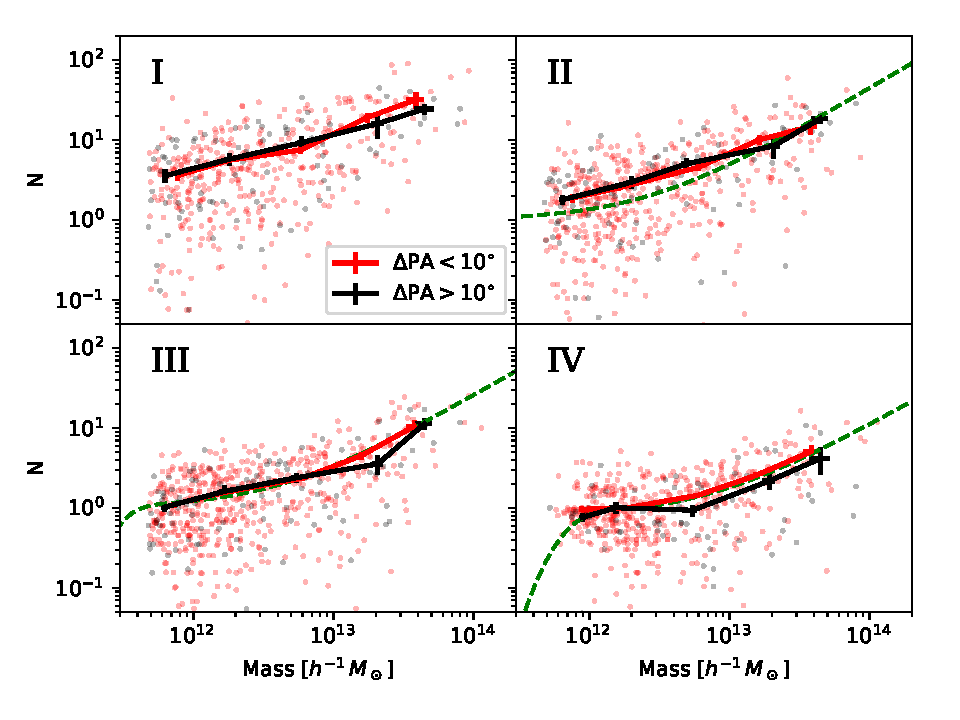
\includegraphics[width=\linewidth]{thesis/latex/halo_assembly_manga/hod_vs_zehavi.pdf}
    \caption[Halo occupation distributions using background subtraction for groups with central galaxies split on $\Delta$PA.]{Halo occupation distributions using background subtraction for groups with central galaxies with $\Delta$PA < 10$^{\circ}$ (red) and $\Delta$PA > 10$^{\circ}$ (black). Panels I, II, III \& IV correspond to a $r$-band magnitude cut of $\leq$ -17, -18, -19 and -20 respectively. The points reflect the estimation for individual groups, with these lines representing the mean with corresponding errors on the mean. In panels II-IV, comparison to HODs estimated directly from clustering with similar magnitude cuts are shown by the green dashed lines \citep[][see text]{zehavi2011}.}
    \label{fig:hod_mpl6}
\end{figure}

\subsection{Discussion}
An important assumption in our motivation has been that gas accretion should originate from cold filamentary flows of the cosmic web. In reality, gas in-flowing into a central galaxy could also result from cooling of the surrounding hot halo and accreting in a more stochastic nature, so we consider that next. 

As introduced in \S \ref{sec:kin_mis}, \citet{lagos2015} explore the origin of kinematic misalignment between gas and stars in ETGs using GALFORM, in comparison with the misaligned field ETG fraction found in ATLAS\textsuperscript{3D} of 42 $\pm$ 6\%  \citep{davis2011a}. They find that using solely galaxy mergers as the source for misaligned cold gas only predicts 2\% of ETGs to have $\Delta$PA > 30$^{\circ}$. Regardless of the time-scales of dynamical friction used, there are simply not enough mergers at $z=0$ to recreate the misaligned fraction observed. To include the effects of smooth gas accretion, they trace its history onto a subhalo along with incident galaxy mergers in their GALFORM model. They follow the angular momentum flips in the constituent cold gas, stars in galaxies and the corresponding dark matter halo using the Monte Carlo simulation prescription of \citet{padilla2014}. This simulation analyses the incident mass with respect to the subhalo, categorising by source (smooth accretion or merger) and constructs a PDF of the expected change in rotational direction for each component: hot halo, cold gas disc and stellar disc. \citet{padilla2014,lagos2015} consider the gas and stellar discs of galaxies to be initially aligned with the surrounding hot halo of gas from which they cooled. When a dark matter halo is accreted, the hot halo is immediately offset from the original rotation, which in time cools to create a misaligned gas disc in the galaxy. Memory of the misalignment can be erased through disc instabilities which use cold gas in the form of a starburst. It should however be noted that this model does not include the relaxation of the gas disc towards the stellar component due to torques. With this in mind any expected misalignment can only be considered an upper limit. \citet{lagos2015} reproduce consistent fractions of misalignment with ATLAS\textsuperscript{3D} by assuming that accretion does not come from a correlated preferential direction. To consider the effect of filamentary `cold mode' accretion on misalignment, the direction of accretion is then correlated on various time-scales and again the expected misaligned fraction is calculated. Assuming an uncorrelated direction of accretion marginally better reproduces observations but more importantly highlights the important role of slower `hot mode' accretion in interpretation. Stochastic accretion onto the galaxy from the hot halo may be the driving factor in misalignment of the gas disc, explaining the lack of correlation with our measures of large-scale environment and halo age. 

\citet{correa2018} investigated the role of cold and hot modes of accretion onto galaxies with respect to the accretion rate onto the host DM halo using the EAGLE suite of hydrodynamical cosmological simulations. In haloes of mass > $10^{12}M_{\odot}$, the two modes of accretion coexist and both contribute to the gas accretion rate on central galaxies. Below this value the cold mode of filamentary flows appear to dominate whereas the hot mode dominates above $10^{12.7}M_{\odot}$ for $z = 0$.  They note that AGN feedback plays an important role on the ability of gas from the surrounding hot halo to cool and accrete and is likely less efficient at high halo masses explaining why hot mode accretion becomes dominant. The ability of cold flows to reach the halo centre is, however, unconfirmed. \citet{nelson2013} find that the majority of gas from cold mode accretion is shock heated as it travels from the DM halo. They compare the differences of the moving mesh code AREPO with the results of GADGET-3 using otherwise identical simulation runs. While gas filaments in GADGET remain collimated and flow coherently to small radii, the same filamentary gas streams in AREPO are heated and become disrupted around  0.25-0.5 r$_{vir}$, boosting the rate of hot gas accretion as a result. The prominence of cold and hot modes of accretion and their subsequent ability to misalign the gas component of a galaxy is rightfully under debate. The lack of correlation of kinematically misaligned galaxies with environments of expected continued accretion could simply indicate that hot mode accretion is dominant in these regimes. 

Another consideration is the visibility of accretion within the effective radii observed in MaNGA. The Primary+ galaxy sample (63\% of MaNGA total including both Primary and Colour Enhanced samples) observes galaxies up to a minimum of 1.5 $R_e$, whereas the Secondary sample (37\% of MaNGA total) goes to a minimum of 2.5 $R_e$. All modes of accretion would be expected to be most visible on the outskirts of the central galaxy which could be further than 1.5-2.5 $R_e$. Below this we could expect gas and stellar components to align on much faster time-scales after an accretion event due to the strength of stellar torques peaking closer to the galactic centre. Despite this, it should be noted that approximately only 20\% of galaxies with $\Delta$PA > 30$^{\circ}$ are from the Secondary sample whereas the fraction of aligned galaxies in the Secondary is as expected from the targeting. 

To assess the impact of changing the observation extent between 1.5 and 2.5 $R_e$ on $\Delta$PA, we consider all Secondary sample galaxies. We find no significant difference in $\Delta$PA when fitting to an aperture 0.6 (1.5/2.5) of the total size of the original IFU extent. This could be a natural limitation of $\Delta$PA being an average property over all radii and hence being preferentially biased towards the rotation of its likely kinematically aligned centre when considering a population excluding recent mergers. The probability of misalignment is linked to the mass of accreted material and lower mass accretion may well propagate to `warps' in the gas velocity map (i.e. $\Delta$PA changing as a function of radius) while maintaining an aligned classification. During visual inspection we found the scenario of a warped gas map while maintaining an undisturbed stellar velocity field to be rare (seen in approximately 20 galaxies). Bars could also be attributed to create warps in velocity fields. \red{Update this statement.} We look to \citet{stark2018} who implement a modified radon transform to characterise PA and its radial variation in the velocity fields of MaNGA for the prevalence of these effects.

Finally, we consider the impact of using a group catalogue to identify central galaxies and estimate halo masses. As discussed in \S\ref{sec:mass_hab}, halo mass is less accurate for small groups, and central mis-classification is more problematic at large halo mass. An estimate of halo mass is only important in one of our tests, where we consider the stellar to halo mass ratio as a proxy for halo formation time. It is possible that errors in halo mass estimates simply averaged out any real signal of $\Delta$PA with the stellar to halo mass ratio. Whereas our two other tests use halo mass estimates to split the data into two populations, the dependence on halo mass values is much reduced, and the Y07 catalogue has been shown to reproduce general trends of galaxy properties as a function of halo mass well \citep{campbell2015}. 
Mis-classification of central galaxies has implications throughout our paper. However at $M_h < 10^{13} M_{\odot}$, where effects of halo assembly are expected to be more prominent, the fraction of groups where stellar ranking results in mis-identification of a satellite as a central is estimated to be well within 10\% by \cite{campbell2015} and \cite{reddick2013}. To consider how 10\% mis-classifications could impact Figure \ref{fig:2d_ratio}, we perform 50 realisations where we remove 10\% of our central sample and replace these with satellites (with their own defined $\Delta$PA) with a consistent distribution in halo mass. This shown in Figure \ref{fig:2d_ratio_realisations} where the additional realisations are plotted in the same colour with different transparency. The overall amplitude of $M_{\ast}/M_{h}$ tends to decrease (especially for low halo mass groups), however there appears to be no noticeable changes in trend. This is expected if a signal is not strong with either population of galaxies.

\begin{figure}
    \centering
	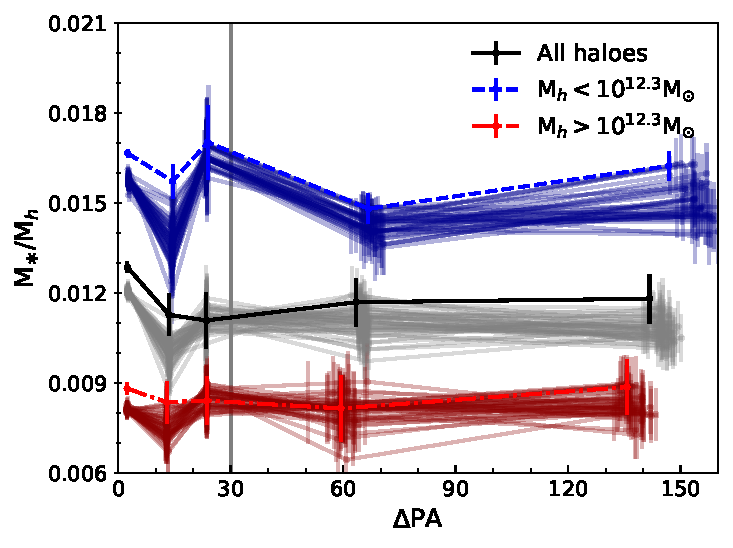
\includegraphics[width=0.7\linewidth]{thesis/latex/halo_assembly_manga/halo_ratio_wsampling.pdf}
    \caption[The same as Figure \ref{fig:2d_ratio} but with 50 realisations where we remove 10\% of our central sample and replace these with satellites]{The same as Figure \ref{fig:2d_ratio} but with 50 realisations where we remove 10\% of our central sample and replace these with satellites. The additional realisations are plotted in the same colour with different transparency with the original distribution overplotted as before. }
    \label{fig:2d_ratio_realisations}
\end{figure}

Although a quantitative assessment of the effects of the group catalogue can only be made using a forward-model approach using mock catalogues we argue, based on the above, that the lack of signal reported in this chapter is more likely due to a lack of physical correlation between halo assembly history and kinematic misalignment measured up to 2.5 $R_e$.

\subsection{Summary}
In this chapter, we considered the visibility of cosmic web accretion and hence halo assembly onto central galaxies in MaNGA. We used the difference in global position angles measured for the stellar and H$\alpha$ velocity fields to classify if a galaxy is kinematically misaligned ($\Delta$PA > 30$^{\circ}$). This chapter is summarised as follows:
\begin{itemize}
\item We first correlated distances to cosmic web features such as nodes and filaments to the aligned and misaligned galaxy samples. We considered the theory that low-mass haloes embedded in filaments (or in close vicinity) find their accretion `stalled' as material moves preferentially towards larger sub-haloes along the filament. This would correspond to aligned central galaxies in low-mass haloes residing closer to filamentary structures. We find that kinematic misalignment holds little or no correlation with the vicinity to nodes or filaments once the effects of morphology, stellar mass and small scale density are considered, as shown in Figure \ref{fig:mh_cw}. 
\item We secondly correlated a proxy for halo age; the central stellar mass to total halo mass ratio, with kinematic misalignment. We explored the idea that large-scale tidal forces dictate the formation time-scales of low-mass haloes ($\lesssim$ 10$^{12.3} M_{\odot}$) which should be reflected both in the halo age but also the likelihood of on-going filamentary accretion being quenched. We found that the magnitude of kinematic misalignment held little or no relation to the proxy of the halo age, as shown in Table \ref{tab:chisq}. 
\item We finally considered the halo occupation distribution as a measure of halo age with older haloes providing more time for satellites to merge and hence decrease the magnitude of the HOD \citep[e.g.][]{zehavi2018}. We estimate the HODs using the background subtraction technique for the aligned and misaligned groups with application of stellar mass weightings between the samples. Regardless of the magnitude limit imposed, we find no statistically significant difference between the groups containing aligned and misaligned galaxies, as seen in Figure \ref{fig:hod_mpl6}. We note in this analysis we split at $\Delta$PA = 10$^{\circ}$ in order to construct a sample size large enough for comparison. While this difference is likely well above the expected average error in $\Delta$PA, internal processes may be erroneously included.
\end{itemize}

We note that the lack of correlation could be indicative that the role of `hot mode' accretion from the cooling of the hot halo may play a far larger role than `cold mode' accretion deriving from the cosmic web flows, even at lower halo masses. The ability of integral field spectroscopy to resolve positions of properties such as gas-phase metallicity and star formation rate histories with respect to the surrounding large-scale environment should shed light on the exact origin of misalignment in future MaNGA studies.

\colorlet{chaptergrey}{black}
%\renewcommand*\sectfont{\color{orange}}
\chapter[Discrete dynamical models of stacked dark matter haloes]{Galaxies as potential tracers: \\ Discrete dynamical models of stacked dark matter haloes in IllustrisTNG}
\label{ch:dyn_mod}
\vspace{-5.25in}
\includegraphics[height=1.18in]{thesis/latex/headers/cw_left.pdf}
\vspace{3in}

%\epigraph{Eat slugs malfoy.}

\section{Introduction}
In the framework of the cosmic web, matter flows preferentially from under-dense to over-dense regions under the influence of the gravitational potential of the cosmic web. In Figure \ref{fig:disperse_matter_path}, we show a diagram of the flow of matter of the cosmic web, using morphological features identified by DisPerSE in IllustrisTNG300. As large-scale structure grows, material moves from voids to the walls that in-case them. These walls are framed by filaments, so that matter travels along walls into the filaments, perpendicular to the filament's major axis. Once in the reference frame of the filament, material moves along its major axis, towards maxima (nodes or clusters). Numerical simulations show that the natural anisotropy of the cosmic web imprints distinct signatures in the orbits of material accreting onto dark matter haloes. Haloes forming at these intersections (saddle) points should experience large degrees of anisotropy since matter is collapsing perpendicular to the filament from the walls but is moving to more dense regimes (nodes) along the direction of the filament itself \citep[e.g.][for galaxy properties in saddle environments]{kraljic2019saddle}. Outside the immediate influence of the cosmic web, lower mass dark matter halos should be able to continue to form matter more isotropically. The decrease in the tidal field strength enables the halos to continue accreting material from smaller scale filamentary structure, leading to more radial orbits.

\begin{figure*}
    \centering
	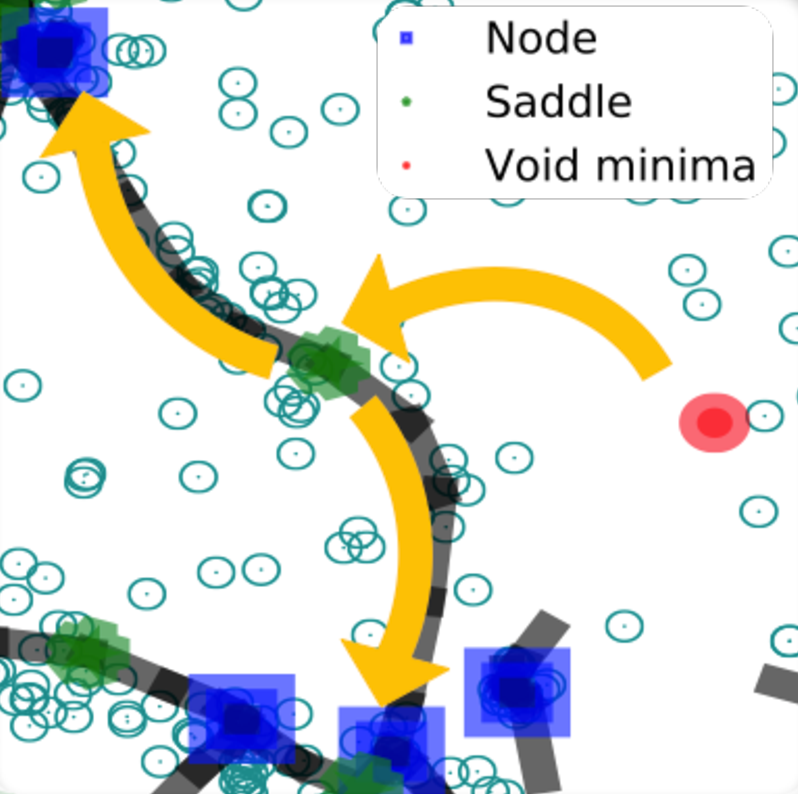
\includegraphics[width=0.5\linewidth]{thesis/latex/dyn_mod_files/disperse_matter_path.pdf}
    \caption{Representation of the flow of matter in large-scale structure. The empty green circles show the galaxy distribution in a slice of IllustrisTNG300 from which DisPerSE has been applied to. Identified nodes (blue squares), saddle points (green stars) and minima (red circles) are shown with filaments (black lines). The yellow arrows show the flow of matter to hierarchically higher mass environments. Mass is sucked out of voids which are funnelled into filaments through walls. Once within filaments, matter moves preferentially along the plane of the filament to the most over-dense regimes: nodes (galaxy groups or clusters). This flow of material inwards (perpendicular) and outwards (parallel) to a given point in the plane of the filament, creates the anisotropy we see in orbits of dark matter; \textit{especially} in saddle points.}
    \label{fig:disperse_matter_path}
\end{figure*}

In numerical simulations, the degree of perturbation from pure isotropic radial accretion is quantified by velocity anisotropy (ratio between velocity moments in tangential and radial directions). This is typically calculated by considering the total population of dark matter particles associated with the halo. On this basis, the orbits have greater tangential dispersion in haloes within environments of both higher tidal field strength and over-density \citep[e.g.][]{faltenbacher2010, shi2015}. \citet{shi2015} characterise the environment through a topological estimator of the tidal field strength, and as discussed in \S\ref{sec:cosmo_numerics}, making a direct link to the geometrically defined cosmic web (i.e. identifying exact positions of filaments, saddle points and other morphological features) is nuanced.  

Baryonic matter is also subject to the gravitational potential of the cosmic web, and, to first order, should trace the same orbits as seen in the dark matter. \citep[][]{garaldi2018} demonstrate this through considering the orbits of all satellite galaxies (albeit including those below the typical mass observable in redshift surveys) within milky way sized haloes. Satellites in those haloes embedded in (or in close vicinity to) large filamentary structure, display distinctly more anisotropic orbits, than those in isolated haloes. Being able to trace the anisotropy though satellite galaxies is promising for observations. However, recovering three dimensional motions for galaxies is extremely difficult.

In this chapter, we aim to trace the flow of dark matter near different morphological features of the cosmic web, through using satellite galaxies as tracers. This chapter contains two main parts; 1) characterising the velocity anisotropy in cosmological simulations in different geometrically defined cosmic web environments, 2) introducing the potential application of discrete dynamical modelling in this context.

In particular, we are interested in the impact of large scale structure on low mass dark matter haloes ($\mathrm{M_{DM} \sim 10^{12}M_{\odot}}$), whose evolution is modulated most strongly by large scale tidal fields, and hence, most likely to trace the anistropy of the cosmic web \citep[e.g.][]{tojeiro2017}. This brings an additional difficulty, as these low mass haloes will host low numbers of satellite galaxies. Using the cosmological simulation of IllustrisTNG300, we stack low mass haloes in different cosmic web environments (voids, saddle points, and filaments) to recover the intrinsic difference in velocity anisotropy. To consider the dynamics within each environment we require $\sim$1000 so we stack in consistent regimes while maintaining orientation and scaling characteristic group lengths. We use this study to motivate the potential to recover the 3D motions of satellites in observations through a new application of the axisymmetric Jeans equations, and hence, the velocity anisotropy of the environment they trace. In section \S\ref{sec:dyn_mod_aniso}, we introduce the data, methodology, and results associated with using satellites galaxies as tracers in different cosmic web environments in IllustrisTNG. In section \S\ref{sec:jam}, we introduce the basics and methodology of discrete dynamical modelling, and highlight the potential for it to be used to recover 3D satellite galaxy dynamics in observations. We also present a re-derivation of the axis-symmetric jeans equations to include gravitational collapse, and removing the steady state assumption. Finally we summarise our findings and conclude in \S\ref{sec:dyn_mod_conclusions}.

\section{Anisotropy in the cosmic web} \label{sec:dyn_mod_aniso}
\subsection{Data}
\subsubsection{IllustrisTNG300}
Throughout this chapter, we base our analysis on galaxies selected from the 300Mpc box of the IllustrisTNG simulation suite. Nominally referred to as IllustrisTNG300 (TNG300), this simulation run follows the evolution of 2500$^3$ dark matter particles ($\mathrm{M_{DM} = 4 x 10^{7}h^{-1}M_{\odot}}$) and 2500$^3$ gas cells ($\mathrm{M_{gas} = 7.6 x 10^{6}h^{-1}M_{\odot}}$. The prescriptions for baryonic physics are consistent with TNG100 (see \S\ref{sec:sim_data_TNG} for further details), however TNG300 provides a far larger cosmological volume, at the cost of spatial resolution.

\subsubsection{Galaxy sample} \label{sec:gal_samp}
As in with TNG100, gravitationally bound structures in TNG300 are identified into haloes and subhaloes through use of a friends-of-friends algorithm \citep{davis85} and the subfind algorithm \citep{springel01} respectively (see \S\ref{sec:sim_data_TNG}). In this work, we select a galaxy sample in TNG300 by considering all $z=0$ (snapshot 99) subhaloes which contain a minimum stellar mass of $\mathrm{M_{\ast} = 10^{8} M_{\odot}}$ within a 3D aperture of 30 comoving kpc from the subhalo centre \citep[as defined in;][]{pillepich18b}. This corresponds to 564,930 unique galaxies which we use for both reconstruction of the cosmic web, and for the satellite tracers in the velocity anisotropy calculations.

In the context of halo assembly, we are particularly interested in isolating the impact of the cosmic web on low mass dark matter haloes. To this effect, we select all galaxies (from our sample above) that reside in a FoF halo of mass $\mathrm{10^{11.5} M_{\odot} < M_{h} < 10^{12.5} M_{\odot}}$, which we use to stack in each cosmological environment as described in \S\ref{sec:stacking}. 

\subsubsection{Cosmological environment}
To identify morphological features of the cosmic web, we make use of DisPerSE (see \S\ref{sec:cosmic_web_intro} for more information). We apply DisPerSE directly to the spatial distribution of our selected galaxy sample in the periodic cube of TNG300. In Figure \ref{fig:disperse_TNG300}, we show the spatial distribution of galaxies for a 10Mpc slice through TNG300, along with the identified filamentary network from DisPerSE.

\begin{figure*}
	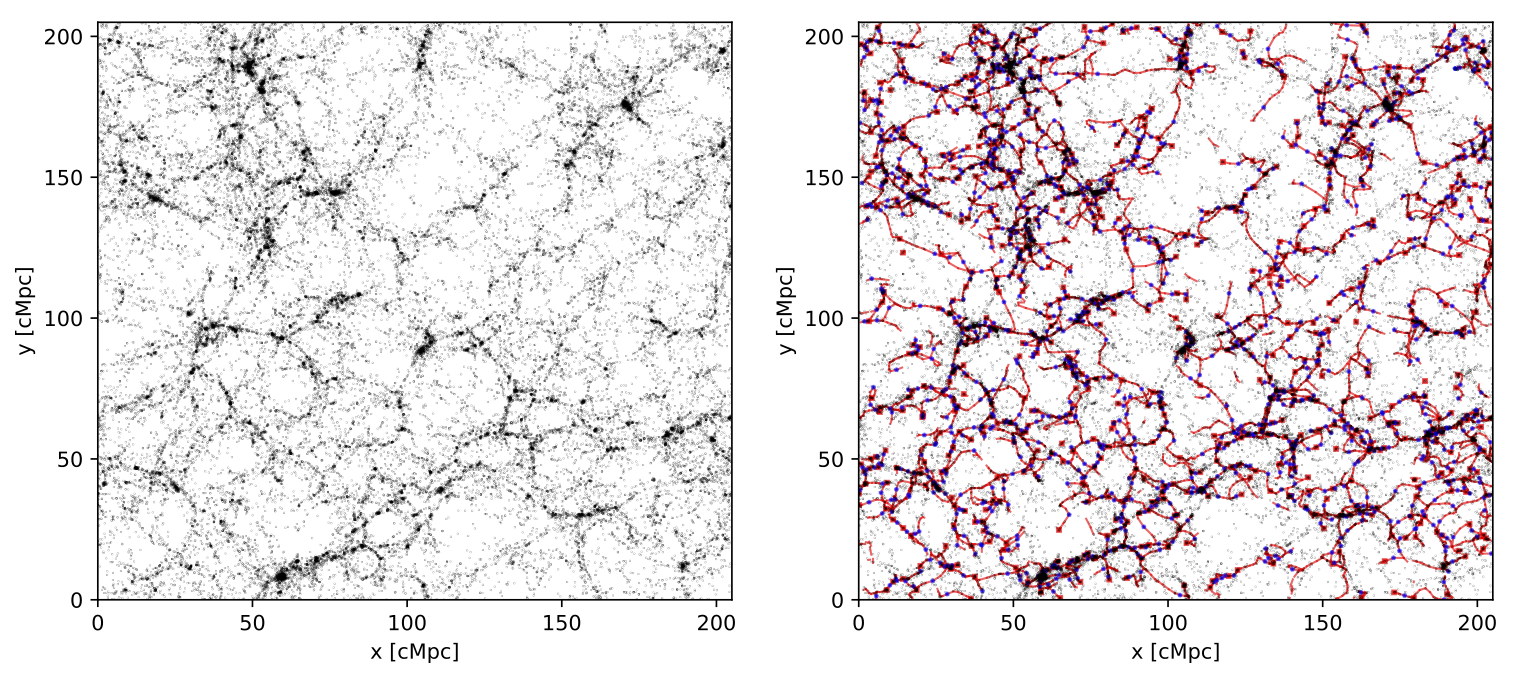
\includegraphics[width=\linewidth]{dyn_mod_files/TNG300-1-SM10-8-slice-galaxy-density-skeleton-comparison.png}
    \caption{Illustration of the filamentary network identified from galaxy positions within a 10 Mpc slice in TNG. The left panel shows the distribution of galaxy ($\mathrm{M_{\ast} > 10^{8}M_{\odot}}$) positions within the slice. The right panel shows the same but with filamentary structure overlaid (red lines). Critical points are also shown such as nodes (red squares) and saddle points (blue stars) highlighting the ensemble which the skeleton connects.}
    \label{fig:disperse_TNG300}
\end{figure*}

Having constructed a skeleton of the cosmic web, we now look to separate the selected haloes into the distinct cosmological environments in which they live. In similarity with \S\ref{sec:cosmic_web_distances}, for each FoF halo (computed from the centre point), the distance to the nearest node ($\mathrm{D_{node}}$), filament segment ($\mathrm{D_{skel}}$) and saddle point ($\mathrm{D_{2-saddle}}$) is found. 

\subsubsection{Stacking of cosmic web environments} \label{sec:stacking}
In order to trace the differences in orbits for different cosmic web environments with satellite galaxies, we need enough tracers to first compute the anisotropy directly, and further, enough to test the feasibility of recovering the anisotropy through dynamical models in observations. Since our focus is on the impact on low mass haloes, we only have a handful (at best) of satellite galaxies to use as tracers. To proceed, we therefore must stack similar haloes in the same topological environment. 

For each environment (node, filament, saddle point) we select all galaxies in FoF haloes with $\mathrm{10^{11.5} M_{\odot} < M_{h} < 10^{12.5} M_{\odot}}$. We take all halos within the selections shown in Table \ref{tab:stacking}. 

\begin{table}
\centering
\begin{tabular}{|l|c|c|c|}
\hline
& Filament & 2-saddle & Void \\ \hline
$D_{node}$ & > 2 Mpc & > 2 Mpc & > 5 Mpc \\
$D_{skel}$ & < 0.5 Mpc  & - - & > 5 Mpc \\
$D_{2-saddle}$ & > 1 Mpc & < 0.75 Mpc & > 5 Mpc \\
Number of galaxies: & 8071 & 941 & 2246 \\
\hline
\end{tabular}
\caption{Selection criteria for stacks in three different environments; filaments, 2-saddle points and voids. Each row shows the distance cut used to select an environment apart from the final row which shows the total number of galaxies selected.}
\label{tab:stacking}
\end{table}

In addition to the distribution of satellites, we also require an assumed dark matter potential for each stacked environment. To construct a reliable dynamical model, all tracers should reside in gravitational potentials that are consistent in overall mass and scale. For every FoF halo that contains a galaxy to be stacked we take the density profile and scale it according to the characteristic group scale as defined by $R_{200}$ (comoving radius of a sphere centered on the FoF halo whose mean density is 200 times the critical density of the Universe). The magnitude of the density profile is scaled according to the total mass contained in the FoF halo and then combined with all density profiles, each with an equal weighting. The stacked FoF halo density profile is finally scaled so that its total mass is equal to the average for all profiles in the stacked population. We then convert the final density profile to the gravitational potential. Each tracer position and velocity is also scaled by the characteristic group scale of its host FoF halo, $\mathrm{R_{200}}$. \red{Should velocity be scaled according to mass or is this accounted for by the scale?}. 
A natural assumption of the axis-symmetric Jeans equations is symmetry around the principal axis of rotation, and hence, it is important to retain directionality while stacking tracers (galaxies) and potentials. In the instance of saddle points and filaments, we use the direction of the nearest filament segment (from saddle to node) to stack galaxy positions/velocities and the gravitational potential around. For those stacked far away from large scale structure (i.e. voids), we use the direction of the overall angular momentum vector of the dark matter in the central subhalo.

\subsection{Velocity anisotropy} \label{sec:velocity_anisotropy}
\subsubsection{Results}
For each environment stack, we first directly compute the anisotropy from the three-dimensional motions of the satellite galaxies. We define two measures of anisotropy, based on the radial and tangential velocity moments. Following \citet{faltenbacher2010}, we refer to the \textit{velocity anisotropy parameter} as such;
\begin{equation} \label{eq:vel_ani_sigma}
\mathrm{\beta_{\sigma}(r) = 1 - \frac{\sigma_t^2(r)}{2 \sigma_r^2(r)} }
\end{equation}
where $\sigma_r^2(r)$ and $\sigma_t^2(r)$ denote the radial and tangential velocity dispersions. Additionally, we also compute the \textit{satellite anisotropy parameter}, motivated in \citet{ZOMGiii} to compute the anisotropy directly from the orbits of satellite subhaloes. This is defined as follows,
\begin{equation}
\beta_{sat}(r) = 1 - \frac{v_{t}^2(r)}{v_{r}^{2}(r)} 
\end{equation}
where $v_{t}(r)$ and $v_{r}(r)$ denote the radial and tangential velocities.

\red{add DM particle only version of this} In Figure \ref{fig:beta_stack}, we show the radial profiles of both $\beta_{sat}$ (left) and $\beta_{\sigma}$ (right) for all satellites in each environment stack. The radial profiles are computed by a set of logarithmically spaced (in radial space) concentric shells, which range from 0 Mpc (from the stack centre, defined by the position of the central galaxy) to 1 Mpc. The number of radial bins are chosen to ensure a reliable measure of anistropy in each shell, which varies between stacks due to varying total numbers of tracers. In each panel we show the profiles for the void (red, dotted), filament (black, dot-dashed) and saddle (green, solid) stacks, accompanied by the average values (grey box) across all radii. 

\begin{figure}
	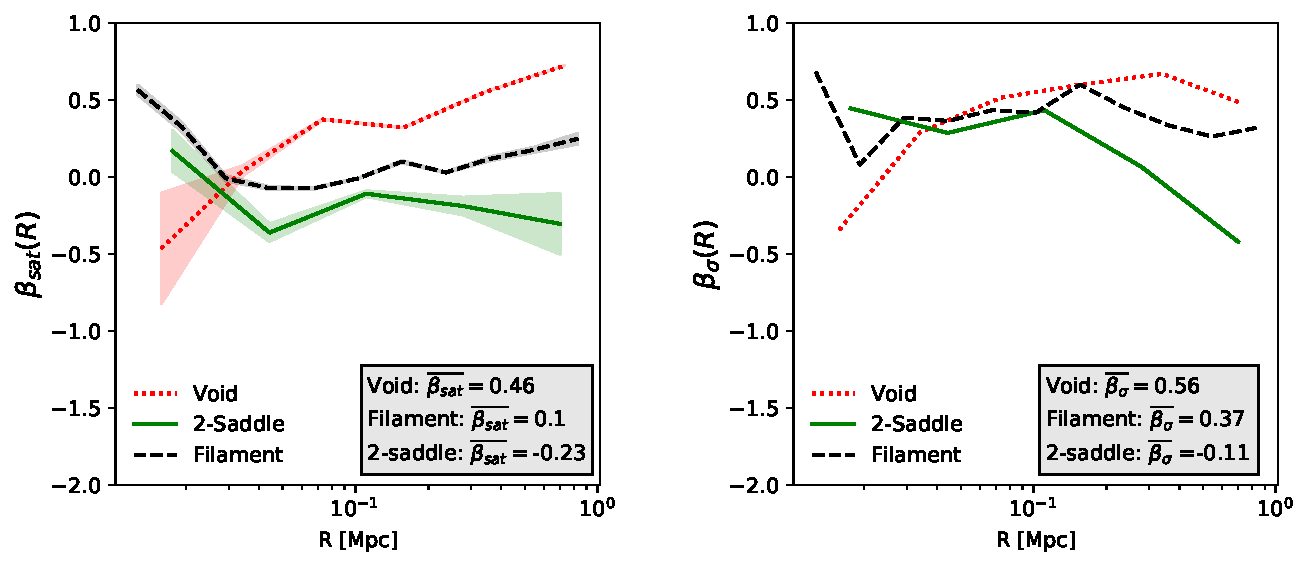
\includegraphics[width=\linewidth]{thesis/latex/dyn_mod_files/disperse_beta_paper.pdf}
    \caption{Velocity anisotropy profiles found from satellite galaxies in the void (red, dotted), filament (black, dot-dashed) and 2-saddle (green, solid) stacks. The left (right) panel corresponds to $\beta_{sat}$ ($\beta_{\sigma}$) with the shaded regions showing error on the mean. The average value for all satellites in each stack is shown in the grey box. For both $\beta_{sat}$ and $\beta_{\sigma}$, there is a clear distinction in orbital anisotropy between environments which increases with radii.}
    \label{fig:beta_stack}
\end{figure}

Starting with the left panel, we find that overall $\beta_{sat}$ is distinctly different between environments ranging from radially biased orbits (voids; positive $\beta_{sat}$) to tangentially biased orbits (saddles, negative $\beta_{sat}$) with intermediate orbits in filaments. As expected, the difference in anisotropy is far more distinct in the outer regions of the halo (i.e. $> 0.1$Mpc), where the impact of large scale tides can take hold over the driving force of the self-gravity of the halo. These differences are also reflected in the dispersions (right panel), where again saddle points host satellites that are on more tangentially biased orbits (particularly in their outer halo) with respect to voids, with orbits in filaments at intermediate values. In both instances, computing average values of orbital anisotropy we find distinct differences between environments. As discussed in \red{\S}, dynamical models require assumptions about the velocity anisotropy (as a parameter in the model). To reduce complexity in the model, it is often better to assume a flat profile in $\beta_{\sigma}$, so it is promising that differences in anisotropy when considering the whole population average. It should be noted that while it is important to retain directionality in stacking for the purpose of dynamical modelling, it has no impact on the direct measures of $\beta_{\sigma}$ and $\beta_{sat}$.

\subsubsection{Discussion}
To interpret our findings, we now place these results in the context of previous studies making use of velocity anisotropy. On a particle level, the orbits within FoF haloes have been shown to be dependent on large scale environment. \citet{faltenbacher2010} used an implementation of the Tree-PM N-body code GADGET2 on-top of the Millenium simulation. They examine the correlation between clustering and halo properties such as shape, concentration, spin, shape of the velocity ellipsoid and velocity anisotropy ($\beta_{\sigma}$). They determine that $\beta_{\sigma}$ is most tightly correlated with the clustering strength, with halos of low velocity anisotropy being more highly clustered and the opposite holding true for haloes with strongly radially biased velocities. 

A possible explanation for more highly clustered haloes exhibiting a relatively larger tangential velocity dispersion is that the impact parameters of the merging sub-haloes are larger due to far more gravitational interactions a short time before accretion. This would lead to a greater dispersion of tangential velocities corresponding to a lower velocity anisotropy. On the other hand, in less clustered regions the gravitational field is dominated by the halo itself naturally leading to more radial in-fall. 

Velocity anisotropy has also been decomposed as a function of tidal environment. \cite{shi2015} investigate how halo dynamical properties are related to their formation histories and hence the tidal environment in which they reside. Figure \ref{fig:shifig11}, shows the relationship of $\beta_{\sigma}$ of particles in central `host' haloes and the tidal field strength in which these haloes reside. In both mass bins there is a clear correlation between $\beta_{\sigma}$ and the first eigenvalue of the tidal tensor (i.e. tidal field strength). As tidal field strength increases, $\beta_{\sigma}$ decreases, showing that again there is a greater dispersion in tangential orbits. 
\begin{figure}
\begin{center}
	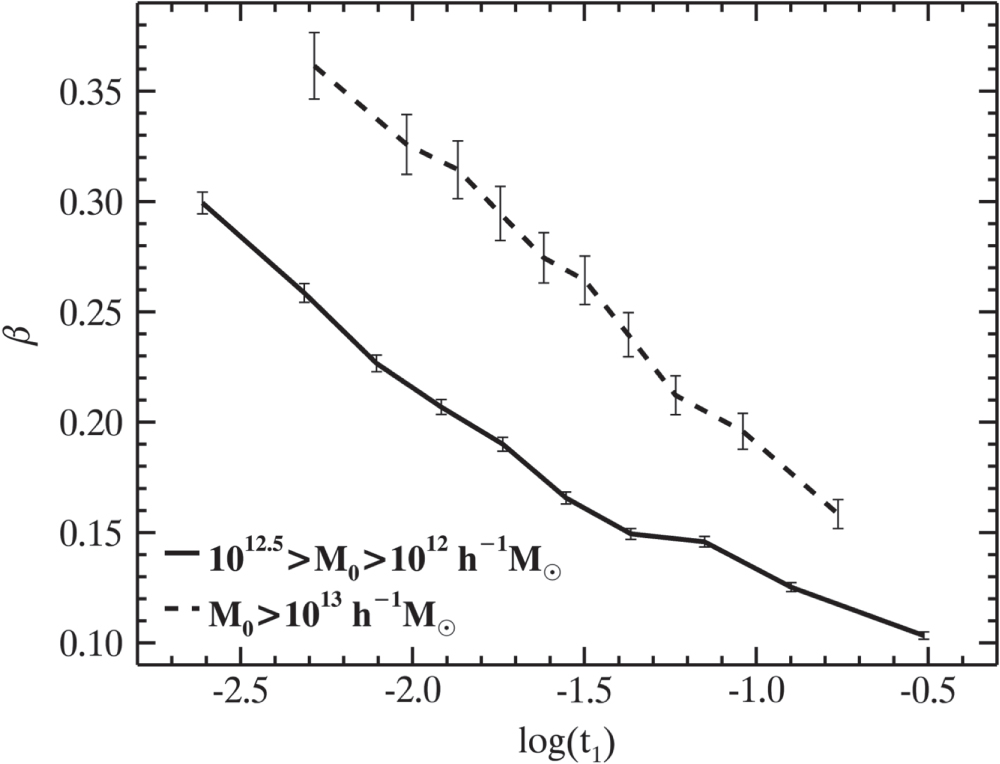
\includegraphics[width=0.5\linewidth]{thesis/latex/dyn_mod_files/shi2015fig11.jpg}
    \caption{Correlation between velocity anisotropy defined by equation \ref{eq:vel_ani_sigma} of host haloes and the first eigenvalue for the tidal field estimator. This plot is shows that as tidal field strength increases, $beta_{\sigma}$ decreases indicating more dispersion in tangential orbits.}
    \label{fig:shifig11}
\end{center}
\end{figure}

Extending this argument to include the impact of the cosmic web, the ZOMG (Zooming in On a Mob of Galaxies) paper series \cite{ZOMGI,ZOMGII,ZOMGiii}, present a set of zoom N-body and hydrodynamical simulations. They follow seven galaxy sized haloes selected on a definition of collapse time which generates strong assembly bias. These haloes are classified as `stalled' or accreting corresponding to the time at which their final mass becomes stable. Stalled haloes correspond to haloes which have become stable at $z \sim 1.5$ whereas accreting haloes are still yet to reach this point. 
The accreting haloes correspond with nodes of the cosmic web and are fed isotropically by radial infall of matter along thin filaments. Conversely `stalled' haloes are embedded in prominent filaments of the large-scale structure. Matter recedes along the filament to starve the early-forming halo as infall only becomes possible from the perpendicular directions. Overall this inflow is balanced by the outflow along the filament leading to no net mass growth. In this instance they follow the orbits on a satellite level rather than particle level. They find that the satellite anisotropy parameter at $z = 0$ is positive for accreting haloes and negative for stalled haloes showing that orbits become more tangentially biased (both in magnitude and dispersion) when low mass haloes are closer to large filamentary structure. Stalled haloes are also found to have a smaller fraction of their mass in sub-structure with respect to the accreting haloes. This can be see as a natural result of a more vibrant recent-accretion history for the later forming haloes. 

Our results are consistent with the idea of tidal forces acting to `stall' accretion leading to more tangentially biased orbits in the outskirts of haloes within filamentary structure. This effect is maximised in close vicinity to saddle points, due to the distinct anisotropy of material flowing in-wards perpendicular to the filament, and once accreted, preferentially along the filament. We show that satellite galaxies \textit{can} be used to trace the orbits within dark matter haloes, and distinct differences can be found between cosmic web environments. In the next section, we introduce the concept of discrete dynamical modelling in the context of the axis-symmetric Jeans equations, and consider the feasibility of applying them to observations, in order to recover their 3D motions, and hence velocity anisotropy.

\section{Potential applications of discrete dynamical models} \label{sec:jam}
Historically, the Jeans equations have served as a powerful tool to convert the observed projected luminosity distribution and kinematics of galaxies (or clusters of stars), to understand the underlying gravitational potential or the 3D de-projected kinematics. Under a series of assumptions, the Jeans equations enable best fitting models to understand further properties about the modelled system. In this section, we briefly introduce the Jeans equations under the assumption of axis-symmetry (\S\ref{sec:jeans_intro}), before re-deriving the equations removing the steady state assumption (\S\ref{sec:jeans_rederivation}). In \S\ref{sec:discrete_dynamical_models} we introduce the concept of dynamical models and motivate the usage in the context of satellite orbits, before summarising and concluding in \S\ref{sec:dyn_mod_conclusions}. 

\subsection{Introduction to the Jeans equations} \label{sec:jeans_intro}
The narrative in this section follows that of \citet{cappellari2008} and \citet[BT henceforth;][]{binneytremaine}, with additional explanation and context where necessary. The phase space distribution of positions ($x_{i}$) and velocities ($v_{i}$) for a set $i$ of tracers (such as stars, IFU spaxels or potentially satellite galaxies) within a massive system (such as a stellar cluster, galaxy or dark matter halo) can be characterised by the distribution function (DF): $f(x,v)$. If make the assumption that the system is in a \textit{steady state} (i.e. $\frac{\partial}{\partial t} = 0$: the system is not collapsing over time - we will return to this assumption later!) and the underlying gravitational potential ($\Phi$) that the tracers are subject to is smooth, then the DF \textit{must} satisfy the steady-state collisionless Boltzmann equation:
\begin{equation}
\sum^{3}_{i=1}\left(v_{i}\frac{\partial f}{\partial x_i} - \frac{\partial \Phi}{\partial x_{i}}\frac{\partial f}{\partial v_{i}} \right) = 0.
\end{equation}
Since $f$ is a function of 6 variables, there are many (infinite) solutions to this equation, so to make use of this in a practical sense, we must make assumptions. One method is to only consider the velocity moments of the DF; i.e. develop Jeans equations. 

\subsubsection{Some assumptions}
The first step in simplifying the solutions is to make use of the natural symmetry of the system. Common assumptions include spheroidal or axial symmetry, since dark matter haloes are often flattened (\red{reference?}), here we make use of the Jeans equations under the assumption of axis-symmetry. We can make our lives easier by transforming to cylindrical polar coordinates $(R,z,\phi)$. In the context of our stacked environments, this corresponds to the radial distance along the axis of stacking ($z$, i.e. direction of nearest filament or rotational axis), the radial distance perpendicular to this ($R$) and the rotation direction around z ($\phi$). The assumption of axial symmetry, allows to us to state that $(\frac{\partial \Phi}{\partial \phi} = \frac{\partial f}{\partial \phi} = 0)$, i.e. symmetric luminous component and potential around the z-axis. The collionless Boltzmann equation (cf. BT equation 4-17) then becomes
\begin{equation}
v_{R}\frac{\partial f}{\partial R} + v_{z}\frac{\partial f}{\partial z} + \left(\frac{v_{\phi}^2}{R} - \frac{\partial \Phi}{\partial R}\right)\frac{\partial f}{\partial v_{R}} -\frac{\partial \Phi}{\partial z}\frac{\partial f}{\partial v_z} - \frac{v_R v_{\phi}}{R}\frac{\partial f}{\partial v_{\phi}} = 0.
\end{equation}

To convert this into something solvable, this equation is multiplied by $v_R$ and $v_z$ respectively and integrated over all velocities to obtain the two Jeans equations \citep[][; BT equation 4-29a,c]{jeans1922}
\begin{eqnarray} \label{basic_jeans1}
\frac{\nu \overline{v_{R}^{2}} - \nu \overline{v_{\phi}^{2}}}{R} + \frac{\partial (\nu \overline{v^{2}_{R}})}{\partial R} + \frac{\nu \overline{v_{R} v_{z}}}{\partial z} = - \nu \frac{\partial \Phi}{\partial R} \\
\frac{\nu \overline{v_{R}v_{z}}}{R} + \frac{\partial (\nu \overline{v^{2}_{z}})}{\partial z} + \frac{\nu \overline{v_{R} v_{z}}}{\partial R} = - \nu \frac{\partial \Phi}{\partial z} \label{basic_jeans2}
\end{eqnarray}
where $\nu$ is the observed luminosity density distribution for the system so that
\begin{equation}
\nu \overline{v_{k}v_{j}} \equiv \int v_{k} v_{j} f d^{3}v.
\end{equation}
We have simplified things by assuming axisymmetry for the steady-state Boltzmann equation but we are not there yet. These equations don't require the potential to be generated by the luminosity density (self-consistency) and they make no assumptions about the form of the DF. Even in a world where we know the potential $\Phi$ (or can make a guess using the surface luminosity and a mass-light ratio) we are left with 2 equations and four unknowns: $\overline{v_{R}^{2}}$,$\overline{v_{z}^{2}}$,$\overline{v_{\phi}^{2}}$ and $\overline{v_{R}v_{z}}$ - i.e. we still can't define a unique solution. 

\subsubsection{Some more assumptions}
The level of velocity dispersion in each dimension of the cylindrical polar coordinate system is quantified by the \textit{velocity ellipsoid}. Dispersion in the $R$ and $z$ planes are fairly intuitive, whereas dispersion in the $\phi$ direction corresponds to orbits moving away from ordered rotation. Since we are discussing an axisymmetric system $(\frac{\partial }{\partial \phi} = 0)$, it makes sense to consider the anisotropy of the velocity ellipse in the R and z directions. In the context of galactic systems, the (R,z) plane is referred to as the meridional plane, terminology that we continue to adopt here.

Mathematically speaking the velocity ellipsoid is defined at every point in the system by the three principal axes arising from the diagonalisation of the dispersion tensor so that
\begin{equation}
\sigma_{ij}^{2} = \overline{v_i v_j} - \overline{v_i v_j} = \frac{1}{\nu} \int (v_i - \overline{v_i})(v_j - \overline{v_j}) f d^3 v.
\end{equation}
To try and visualise this we can draw the distribution of velocity dispersions: $\sigma_R$ and $sigma_z$ for each position in the meridional plane. For example, if we were to do this for a galaxy bulge the shape of this (velocity ellipsoid projection) would be spherical, whereas if it was considered in the disk plane it would be an ellipse flattened in the z-direction. 

Our discussion so far has made one key simplifying assumption about the velocity ellipse; its principal axes are aligned with our coordinate system i.e $\overline{v_R v_z} = 0$. Physically this means that velocities in the R and z directions are not correlated and hence our velocity ellipsoids are not tilted in the meridional plane. For galactic systems, this is a poor assumption going above the thin-disk plane since many orbits in the Milky way trail towards the centre. Still, we can live with this poor assumption since the majority of the orbits lie in the thin disk or the spheroidal bulge. \red{discuss how this is relevant for satellite galaxies.}

After assuming our velocity ellipsoids are not tilted in the meridional plane, we now make a further assumption that their axis ratio is fixed and defined by:
\begin{equation} \label{beta_z}
\beta_z = 1 - \frac{\overline{v_{z}^2}}{\overline{v_{R}^2}}.
\end{equation}
Again using a galaxy as an example, a bulge would have $\beta_z \approx 0$ since $\overline{v_z^2} \approx \overline{v_R^2}$, whereas a disk would have $\beta_z \approx 0.5$ since $\overline{v_z^2} < \overline{v_R^2}$. In principal we can allow $\beta_z$ to vary as function of R, since it can be defined for each MGE component (see next section). In reality we want to minimise free parameters and either set it to a mean value for the whole system or a subset of tracers (e.g. for each of bulge and disk stars). 

Mathematically speaking, defining our system to be axisymmetric implies that $\overline{v_{R}} = \overline{v_{z}} = 0$. Therefore the dispersions in these directions are simple: $\sigma_{z}^2 = \overline{v_z}^2$ and $\sigma_{R}^2 = \overline{v_R}^2$. Quantifying $\sigma_{\phi}$ is trickier since we need to find the average rotation, leading to the definition of the rotation parameter $\kappa$ \red{reference to somewhere}. 

Implementing these assumptions (where $b = 1/\beta_z$) and using the boundary condition that $\nu \overline{v_z^2} = 0$ as $z \to \infty$, we can define our Jeans equations to reproduce the second velocity moments in $z$ and $\phi$:
\begin{eqnarray} \label{jeans1}
\nu \overline{v_z^2}(R,z) = \int^{\infty}_{z} \nu \frac{\partial \Phi}{\partial z} dz \\
\nu \overline{v_{\phi}^2}(R,z) = b \left[ R \frac{\partial (\nu \overline{v_z^2})}{\partial R} + \nu v_{z}^2\right] + R\nu \frac{\partial \Phi}{\partial R} . \label{jeans2}
\end{eqnarray}
One final caveat regarding the implementation of the Jeans equations in this way, is that the solution satisfying these may not correspond to a physical (positive) DF. To assess the validity of the solutions for a given system model we can compare these predicted moments with the observed distributions for our tracers. However to do so we need to parametrise both the form of the potential $\Phi$ and the luminous surface density $\nu$.

\subsubsection{Steady state assumption for satellite dynamics}
One key assumption throughout this introduction is that the system (dark matter halo) is in a \textit{steady state}. This assumes that the satellites (or subhaloes) used as tracers are virialised and the system is relaxed. Observations \citep[e.g.][]{mamon2005} and N-body simulations \citep[e.g.][]{mahajan2011}, however, have shown that virialised clusters (or groups) are surrounded by in-fall zones from which the subhaloes move into the system, as predicted in \citet{gunn1972}. Assuming that the overall dark matter halo is also under collapse in these regions, accretion with significant radial motion \textit{breaks} the steady state assumption, and hence a method to account for this additional peculiar in-fall motion, and, the impact of the Hubble expansion must be included in our equations of motion.

One potential solution to overcome the difficulties of a system in a non steady state is identify and remove sub-populations of tracers when evaluating the best fitting dynamical model (see; \S\ref{sec:discrete_dynamical_models}). In this instance, those with significant in-fall velocities on the outskirts can be down-weighted or removed from the model. Despite this, in Figure \ref{fig:beta_stack}, we showed that the difference in anisotropy between different environment is most distinct in the outskirts of the halo, away from the impact of self-gravity, so approach is risky, as it may remove the tracers which display the majority of this signal.

Instead, an alternative is to relax the steady state assumption in our Jeans equations (equations \ref{basic_jeans1} \& \ref{basic_jeans2}). By generalising the standard Jeans formalism, we can include additional terms such as the peculiar in-fall motions of galaxies, and cosmological expansion. In \S\ref{sec:jeans_rederivation} we re-derive the Jeans equations to include these additional terms. Of particular relevance to this work is \citet{falco2013}, who introduce and implement a generalised set of Jeans equations, however, under the assumption of spherical symmetry. In this work, they include additional terms corresponding to the radial collapse (or in-fall) of galaxies, Hubble expansion, and contributions from background cosmology. They find that adapting the Jeans equations, enables recovery of key parameters (such as the radial velocity dispersion) to 2 virial radii and above. 

\subsection{Generalised Jeans equations in cylindrical coordinates} \label{sec:jeans_rederivation}
In standard cylindrical coordinates (R,z,$\phi$) under the assumption of axial symmetry (so that; $\partial \Phi / \partial \phi = \partial f / \partial \phi = 0$) we find the collisionless Boltzmann equation to be (cf. BT equation [4-17]): 
\begin{equation} \label{eq:CBE}
\frac{\partial f}{\partial t} + v_R \frac{\partial f}{\partial R} + v_z \frac{\partial f}{\partial z} + \left[\frac{v_{\phi}^2}{R} - \frac{\partial \Phi}{\partial R}\right] \frac{\partial f}{\partial v_R} - \frac{v_R v_{\phi}}{R} \frac{\partial f}{\partial v_{\phi}} - \frac{\partial \Phi}{\partial z} \frac{\partial f}{\partial V_z} = 0.
\end{equation}

Without making the usual assumptions of steady state, we multiply equation \ref{eq:CBE} by $v_{R}$ and $v_z$ respectively and integrate over all velocities to obtain (Jeans 1922, BT equation [4-29a,c])
\begin{align} \label{eq:j_vr}
\frac{\partial (\nu \overline{v_R})}{\partial t} + \frac{\partial (\nu \overline{v_R^2})}{\partial R} + \frac{\partial (\nu \overline{v_R v_z})}{\partial z} + \nu \left[ \frac{\overline{v_R^2} - \overline{v_{\phi}^2}}{R} + \frac{\partial \Phi}{\partial R}\right] &= 0\\ \label{eq:j_vz}
\frac{\partial (\nu \overline{v_z})}{\partial t} + \frac{\partial (\nu \overline{v_R v_z})}{\partial R} + \frac{\partial (\nu \overline{v_z^2})}{\partial z} + \nu \frac{\overline{v_R v_z}}{R} + \nu \frac{\partial \Phi}{\partial z}&= 0.
\end{align}
where we use the following notation
\begin{align}
\nu &\equiv \int f d^3 v \\
\nu \overline{v_k v_j} &\equiv \int v_k v_j f d^3 v .
\end{align}
Similarly we can derive the continuity equation in cylindrical coordinates by integrating \ref{eq:CBE} over all velocities (cf. BT [4-28])
\begin{equation} \label{eq:contin}
\frac{\partial \nu}{\partial t} + \frac{1}{R}\frac{\partial (R \nu \overline{v_R})}{\partial R} + \frac{\partial (\nu \overline{v_z})}{\partial z} = 0.
\end{equation}
We wish to now go beyond the assumption of steady state and allow net radial motion due to the infall and collapse of dark matter haloes (i.e. $\overline{v_r} \neq 0$, $\overline{v_z} \neq 0$). The second order velocity moments therefore can be written as:
\begin{align} \label{eq:vr}
\overline{v_R^2} &= \sigma_R^2 + \overline{v_R}^2 \\ \label{eq:vz}
\overline{v_z^2} &= \sigma_z^2 + \overline{v_z}^2
\end{align}
We can now make use of the continuity equation \ref{eq:contin} and rewrite the first term in \ref{eq:j_vr};
\begin{align}
\frac{\partial ( \nu \overline{v_R})}{\partial t} &= \nu \frac{\partial \overline{v_R}}{\partial t} + \overline{v_R} \frac{\partial \nu}{\partial t} \\
&= \nu \frac{\partial \overline{v_R}}{\partial t} - \overline{v_R}\frac{\partial (\nu \overline{v_z})}{\partial z} - \frac{\nu}{R}\overline{v_R}^2 - \overline{v_R} \frac{\partial (\nu \overline{v_R})}{\partial R}.
\end{align}
We can also rewrite the second term in equation \ref{eq:j_vr} through use of equation \ref{eq:vr} and the product rule; 
\begin{align}
\frac{\partial ( \nu \overline{v_R^2})}{\partial R} &= \frac{\partial (\nu \sigma^2_R)}{\partial R} + \frac{\partial ( \nu \overline{v_R}^2)}{\partial R} \\
&= \frac{\partial (\nu \sigma^2_R)}{\partial R} +  \overline{v_R}\frac{\partial (\nu \overline{v_R})}{\partial R} + \nu \overline{v_R} \frac{\partial \overline{v_R}}{\partial R}.
\end{align}
Re-introducing these terms and using a similar method for the $v_z$ moment, the Jeans equations (\ref{eq:j_vr},\ref{eq:j_vz}) can be rewritten as
\begin{multline}
\nu \left[\overline{v_R}\frac{\partial \overline{v_R}}{\partial R} + \frac{\partial \overline{v_R}}{\partial t} \right] - \overline{v_R} \frac{\partial (\nu \overline{v_z})}{\partial z} + \frac{\partial (\nu \sigma_R^2)}{\partial R} + \frac{\partial (\nu \overline{v_R v_z})}{\partial z} + \nu \left[ \frac{\sigma_R^2 - \overline{v_{\phi}^2}}{R} + \frac{\partial \Phi}{\partial R}\right] = 0
\end{multline}
\begin{multline}
\nu \left[\overline{v_z}\frac{\partial \overline{v_z}}{\partial z} + \frac{\partial \overline{v_z}}{\partial t} \right] - \overline{v_z} \frac{\partial (\nu \overline{v_R})}{\partial R} + \frac{\partial (\nu \sigma_z^2)}{\partial z} + \frac{\nu \sigma_{Rz}^2}{R} + \nu \frac{\partial \Phi}{\partial z} = 0 
\end{multline}
where we have used that $\overline{v_z v_R} = \sigma_{Rz}^2 + \overline{v_R} \ \overline{v_z}$. These reduce to the usual form of the Jeans equations under the steady state assumption but due to this inclusion of non-equilibrium, we find three additional terms in both relating to the mean radial motion of galaxies in both the $z$ and $R$ directions. \red{need to take further and introduce what the additional terms could correspond to - i.e. in-fall, hubble expansion etc.}

\subsection{Discrete dynamical models} \label{sec:discrete_dynamical_models}
\red{need to make segway about how to adapt Jeans equations to produce first order velocity moments (as in Watkins et al. 2013.}
We now introduce the likelihood function which can be evaluated for a set of tracers (galaxies) in a system (stacked dark matter halo) for our choice of generalised or steady state Jeans equations. As an introduction, we follow the formalism of discrete dynamical modelling introduced in \citet{watkins2013} in the instance where full 3D motions and velocities are know for the tracer population. We then adapt the likelihood function and solutions since in observations we would not be equipped with 3D velocities for galaxies. This issue can be abridged by considering additional information about the tracers (i.e. tracers with different morphological or colour properties may have dynamical properties and hence can be separated and modelled differently), and adapting the likelihood function \citep[e.g.][]{zhu16sculptor}.

\red{need to include description of functional form for the gravitational potential (from paper draft?), first order velocity moment computation, and MGE stuff.}

\subsubsection{An ideal world}
As an introduction, we first consider the form of the likelihood function for a single population of tracers where we know the complete dynamical characteristics for (i.e. we know their 3D positions and velocities). This discussion follows \citet{watkins2013} with application to the globular cluster $\omega$ Centauri, however we try and keep the terminology here as general as possible. If we have a data set of N tracers such that the $i$th tracer has coordinates $x_{i}'= (x'_{i},y'_{i})$ and velocities $v_{x',i} \pm \sigma_{v_{x',i}}, v_{y',i} \pm \sigma_{v_{y',i}}$ and $v_{z',i} \pm \sigma_{v_{z',i}}$, where $x'$ is the projected major axis direction, $y'$ is the projected minor axis direction and $z'$ is the line of sight direction. We can then describe the velocity vector \textbf{$v_{i}$} and the error matrix \textbf{$S_{i}$} such that,
\begin{equation}
\boldsymbol{v}_{i} = (v_{x',i},v_{y',i},v_{z',i}) \quad , \quad \boldsymbol{S}_{i} = \begin{bmatrix} \sigma_{v_{x',i}} & 0 & 0 \\ 0 & \sigma_{v_{x',i}} & 0 \\ 0 & 0 & \sigma_{v_{z',i}} \end{bmatrix}
\end{equation}
assuming uncorrelated errors.

Suppose we have a set of evaluated Jeans equations (\textit{models}; described by a set of parameters $\boldsymbol{\Theta}^{sys}_{j}$) and we want to find which one provides the best prediction to our data set. For a given model with a particular parameter set $j$, then the likelihood of observing a tracer $i$ is given, 
\begin{equation}
\mathcal{L}^{sys}_{ij} = p (\boldsymbol{v}_{i}|\boldsymbol{x}'_{i},\boldsymbol{S}_{i},\boldsymbol{\Theta}^{sys}_{j})
\end{equation}
An important point to note is that position information is taken to be prior information and therefore the probability distribution for each tracer is velocities only. The positions of each tracer is required to generate the expected distribution of velocities from the model, and hence evaluate the fit. The total likelihood $\mathcal{L}^{sys}_{j}$ of a given model is then the product of the model likelihoods for all tracer velocities given their positions:
\begin{equation}
\mathcal{L}^{sys}_{i} = \prod^{N}_{i=1} \mathcal{L}^{sys}_{ij}
\end{equation}
For chain convergence in finding the best model through sampling, it is easier to work with log-likelihoods $\ell_j = ln\mathcal{L}_{j}$. The best model is one that therefore maximises $\ell_j$. 

We now need a way of dealing with tracers that aren't actually part of system (i.e. galaxies in the foreground or background and hence not associated with the stack/halo). To do so we complicate our likelihood function with an additional component such that, 
\begin{equation}
\mathcal{L}_{ij} = \eta_{i}\mathcal{L}^{sys}_{ij} + (1-\eta_i)\mathcal{L}_{ij}^{bg}
\end{equation}
where $\mathcal{L}^{bg}_{ij}$ is the likelihood for the background model with parameters $\boldsymbol{\Theta}^{bg}_{j}$. Our entire parameter set $\boldsymbol{\Theta}_{j}$ therefore comprises of $\boldsymbol{\Theta}^{sys}_{j}$ and $\boldsymbol{\Theta}^{bg}_{j}$. $\eta_{i} = 1$ if the tracer is a member of the system and $\eta_{i} = 0$ if the tracer is part of the background. Since we don't know which tracers are contaminants (unless we want to return to cutting our data), this would add N extra parameters to $\boldsymbol{\Theta}_{j}$ and hence make modelling very difficult. Instead it makes sense to introduce a mixture model that combines the system and background likelihoods:
\begin{equation}
\mathcal{L}_{ij} = m_{i}(\boldsymbol{x}'_{i})\mathcal{L}^{sys}_{ij} + [1 - m_{i}(\boldsymbol{x}'_{i})]\mathcal{L}^{bg}_{ij}
\end{equation}
where $m_{i}(\boldsymbol{x}'_{i}) = p(\eta_{i} = 1| \boldsymbol{x}'_{i})$ is the prior probability that the tracer is part of the system given its position. To find the posterior membership probability for each tracer in a given model we can write,
\begin{equation}
m_{i} = p(\eta_i = 1) = \frac{m_{i}\mathcal{L}_{ij}^{sys}}{m_{i}\mathcal{L}_{ij}^{sys} + (1 - m_i)\mathcal{L}^{bg}_{ij}}
\end{equation}

A necessary component of sampling to find the best fitting model parameters is the construction of priors. Following the discussion of \citet{watkins2013}, we considered membership priors $m_i$ which are entirely dependent on the galaxy's position (i.e. $m_{i}(\boldsymbol{x}'_{i})$). However, if we know expected properties about the typical galaxies in the system we could also include things such as colours and SFR. 

Assuming we have a functional form for the projected luminous surface density of our system, and our unwavering assumption of our system being elliptical in shape (due to the assumption of axial symmetry), it is then natural that we would expect a given tracer near the projected centre to have a higher membership probability than if it were on the outskirts. Assuming that the luminous surface density $I$, is proportional to number surface density $dN_{sys}$ we can write our prior probability of system membership as:
\begin{equation}
m_{i}(\boldsymbol{x}'_{i}) = \frac{dN_{sys}(\boldsymbol{x}'_{i})}{dN_{sys}(\boldsymbol{x}'_{i}) + dN_{bg}(\boldsymbol{x}'_{i})}
\end{equation}
where d$N_{bg}$ is the background surface density. Unfortunately we don't know $dN_{bg}(\boldsymbol{x}'_{i})$, however we can make a reasonable guess\footnote{This is a reasonable guess for star cluster scales. We may have to be careful when thinking about this on cosmic web scales. Do we have reason to believe that foreground/background galaxies should be completely uniform?} that it be assumed to be constant across the system and is equal to a fraction $\epsilon$ of the central system, number surface density $dN_{0} = dN_{sys}(0,0)$. The prior on system membership then becomes
\begin{equation}
m_{i}(\boldsymbol{x}'_{i}) = \frac{dN_{sys}(\boldsymbol{x}'_{i})}{dN_{sys}(\boldsymbol{x}'_{i}) + \epsilon dN_{0}}
\end{equation}
where $\epsilon$ will be included as a free parameter in $\boldsymbol{\Theta}_{j}$.

So to summarise the key components of constructing a likelihood function for a set of discrete tracers: 
\begin{itemize}
    \item We are equipped with positions and velocities for our tracers.
    \item We have a likelihood function for a given model with parameters $\boldsymbol{\Theta}_{j}$ which can deal with tracers not being part of the system.
    \item We can evaluate the likelihood function if we consider our tracer positions as prior information and then estimate the velocity moments from the Jeans equations and compare to the observed values.
\end{itemize}
\textit{But aren't Jeans equations, equations not models?} Well, yes. To proceed we assume that the velocity distribution predicted by the model is a Gaussian (trivariate if 3D) \todo{Is a gaussian a sensible assumption? Lange+18} with mean velocity $\boldsymbol{\mu}_{i}^{sys}$ and covariance $\boldsymbol{\mathcal{C}}_{ij}^{sys}$ at $\boldsymbol{x}_i'$. \textit{In doing this, our results are no longer independent of the form of the DF}. The likelihood can then be written, 
\begin{align*}
\mathcal{L}_{ij}^{sys} &= p(\boldsymbol{v}_i|\boldsymbol{x}_{i}',\boldsymbol{S}_i,\eta_i=1,\boldsymbol{\mu}_{i}^{sys},\boldsymbol{\mathcal{C}}_{ij}^{sys}) \\ &= \frac{\exp{\left[-\frac{1}{2}(\boldsymbol{v}_i - \boldsymbol{\mu}_{ij}^{sys})^{T}(\boldsymbol{C_{ij}^{sys}} + \boldsymbol{S}_i)^{-1}(\boldsymbol{v}_i - \boldsymbol{\mu}_{ij}^{sys}) \right]}}{\sqrt{(2\pi)^{n}|(\boldsymbol{C}_{ij}^{sys}+\boldsymbol{S}_i)|}}
\end{align*}
where n is the rank of $\boldsymbol{S}_i$, for objects with 3D velocities $n=3$.\todo{Derivation of first-order velocity moments?} Remember that we assumed our observed velocity errors are uncorrelated (and Gaussian!). We also assume that the background model predicts a multivariate Gaussian velocity distribution. Our Jeans equations will always generate 3D velocity predictions but this doesn't necessitate that we can only use tracers with 3D velocities. 

\subsubsection{The likelihood function with 1D velocities}
For most situations we will not be blessed with 3D velocities for our tracer population. In particular, if we use galaxies as tracers we will only be equipped with line-of-sight velocities. Before despairing, we recall that we can generalise our likelihood function to not only include spatial information but also population properties such as metallicities/colours/sSFR (referred to as `chemo' or chemical properties henceforth for the sake of consistent nomenclature between star clusters and galaxies). 

In this case, we can consider different tracer populations following the same gravitational potential, but each with its own chemical, spatial and dynamical properties. In principal, this means we can generate models (Gaussians for velocity moments) from the Jeans equations for as many as different populations as we like. This only really worthwhile doing if your populations are \textit{distinct}; i.e. they can actually be split by a `chemo' property and show distinctly different dynamics and spatial distribution. 

For simplicity lets consider $k=2$ populations, consisting of a low SFR and high SFR population of satellite galaxy tracers (for example). This discussion follows \citet{zhu16sculptor}, on which we base on our modelling. For each population k of tracers, we can adopt a Gaussian distribution in SFR $(SFR^{k}_{0},\sigma^{k}_{SFR})$. Given a tracer $i$ with measured SFR $SFR_i \pm \delta SFR_i$, the \textit{chemical} probability that is belongs to population k is then,
\begin{equation}
P_{chm,i}^{k} = \frac{1}{\sqrt{2\pi [(\sigma^{k}_{Z})^2+ \delta SFR_{i}^2]}}\exp{\left[-\frac{1}{2}\frac{(SFR_{i}-SFR^k_0)^2}{(\sigma^k_SFR)^2+\delta SFR_i^2}\right]}. 
\end{equation}

We can also define each population to have its own spatial distribution through the observed surface number density $\Sigma^k(x',y')$. Given a satellite tracer $i$ at position $(x_i',y_i')$, the spatial probability for population k is
\begin{equation}
P^{k}_{spa,i} = \frac{\Sigma^k(x'_i,y'_i)}{\Sigma_{sys}(x_i',y_i')+\Sigma_{bg}}
\end{equation}
where $\Sigma_{sys}$ is the surface number density for all combined populations belonging to the system, excluding the background surface number density $\Sigma_{bg}$, which again we can assume to be a constant fraction $\epsilon$ of the central object surface number density. 

To decompose $\Sigma_{sys}$ into a set of $\Sigma_{k}$ we consider that the number surface density for the system can be expanded into a set of M two-dimensional Gaussians. We can then consider that each Gaussian $j$ contributes a fraction $h^{k}_{j}$ to the surface number density of a given tracer population so that
\begin{equation}
\Sigma^{k}(x',y') = \sum^{M}_{j=1} \frac{L_j}{2\pi \sigma^2_j} \exp{\left[-\frac{x'^2 + y'^2 /q'^2_j}{2\sigma^2_j}\right]}
\end{equation}
where $L_j,\sigma_j,q'_j$ are the total luminosity, dispersion and projected flattening of each Gaussian $j$. If we impose that $\sum^k h^k_j = 1$, then for two populations; low and high SFR we can write if $h^{high SFR} = h_j$ then $h^{low SFR} = 1 - h_j$ for each Gaussian. We can constrain the fraction $h_j$ both spatially and dynamically since the velocity distribution is dictated by both the gravitational potential and the surface number density.

Finally we can define the dynamical probability in a similiar manner as we did where we had full 3D velocity information. For a satellite tracer $i$ with a line-of-sight velocity $v_{z',i} \pm \delta v_{z',i}$, the dynamical probability for a given population $k$, is a Gaussian distribution centred on the Jeans equation prediction $\mu^k_i$ with velocity dispersion $\sigma^k_i$ such that
\begin{equation}
P^k_{dyn,i} = \frac{1}{\sqrt{(\sigma^k_i)^2+ (\delta v_{z',i})^2}} \exp{\left[-\frac{1}{2}\frac{(v_{z',i}-\mu^k_i)^2}{(\sigma^k_i)^2 + (\delta v_{z',i})^2}\right]}.
\end{equation}
\subsubsection{Including contaminants again}
If we know anything about our contaminant population, we can include it in the probability model for the background. As an example we can adopt a Gaussian distribution $(SFR_0^{bg},\sigma_{SFR}^{bg})$ for SFR. As before, we can assume the background surface number density to be uniform across the system, characterised by $\epsilon$. Finally, since we are including velocity in membership probability we can assume the contaminant's velocity to be systematic with respect to the system distributed as a Gaussian $(\mu_0^{bg}=-V_{sys},\sigma_0^{bg})$. 
\subsubsection{Total probability}
Combining all of this, the probability for a tracer $i$ belonging to a given population k can be written as
\begin{equation}
P_i^{k} = P_{spa,i}^k P_{chm,i}^k P_{dyn,i}^k 
\end{equation}
where $k$ in this case refers to our system populations and background. The relative probability for each population can also be described 
\begin{equation}
P'^k_i = P^k_i / \sum^k P^k_i
\end{equation}
which allows us to identify a tracer to a given population or the background.

To evaluate a set of models defined by parameters $\boldsymbol{\Theta}$, we can find the total likelihood for a tracer $i$ found by the sum of these probabilities such that
\begin{equation}
\mathcal{L}_i = \sum_{k \neq bg} P^{k}_{spa,i} P^{k}_{chm,i} P^{k}_{dyn,i} + \left(1 - \sum_{k \neq bg} P^{k}_{spa,i} \right) P^{bg}_{chm,i} P^{bg}_{dyn,i}.
\end{equation}
We then calculate the total likelihood $\mathcal{L} = \prod^N_{i=1} \mathcal{L}_i$ of all N tracers. This total likelihood $\mathcal{L}$ or log-likelihood $ln \mathcal{L}$ are therefore the quantities we would like to maximise. To summarise, the fit of each uniquely defined model is evaluated by a combination of the spatial, chemical and dynamical probabilities for the complete set of tracers in the system. The spatial probability $P^{k}_{spa,i}$ for each tracer $i$, is defined by the likelihood of it belonging to the observed spatial distribution of the tracer population. The chemical probability $P^{k}_{chem,i}$ for each tracer $i$, is defined by the likelihood that it has chemical properties (e.g. SFR) consistent with its parent sub-population. The dynamical probability $P^{k}_{dyn,i}$ for each tracer $i$, evaluates the model fit prediction of its velocity (predicted by using its position as a prior) relative to its observed. The best fit model is evaluated by considering if each tracer $i$ belongs to each sub-population \textit{and} the background population, and hence has no weighting in the model evaluation.

\section{Discussion and Summary} \label{sec:dyn_mod_conclusions}
In this chapter, we introduced the idea of tracing the flow of dark matter in different environments of the cosmic web through a novel application of discrete dynamical modelling. 

In the first half of the chapter (\S\ref{sec:dyn_mod_aniso}), we used the cosmological hydrodynamical simulation of IllustrisTNG-300 to geometrically identify different cosmic web environments. In each of the environments, we stacked satellite galaxies (\red{and their underlying distribution of dark matter}) to understand how the dynamical properties of haloes are modulated by the cosmic web. We demonstrated that low mass haloes in close vicinity to filaments host orbits that are typically more tangentially biased relative to haloes in void environments. This effect is seen most strongly for haloes positioned close to saddle points in the filaments. The environmental effect is seen most prominently on the outskirts of the haloes, outside of the effect of self-gravity and interactions.

In the second half of this chapter (\S\ref{sec:jam}), we introduced the formalism for applying the Jeans' equations to stacked haloes in observations to recover the three dimensional orbits of the satellites. This technique represents a significant opportunity to identify orbits of the underlying gravitational potential (i.e. dark matter) and how this could be modulated by the position within the cosmic web. 

The difficulty in applying this technique to observations is two-fold. Firstly identification of the cosmic web must be accurate, and reconstruction from sparsely sampled redshift surveys such as SDSS may introduce significant noise. This sampling also makes accurate group identification difficult. Secondly, due to the magnitude limit of SDSS, only reasonably bright satellites will be observed and hence a large number of group will need to be stacked. Solutions to both of these problems could lie with the Dark Energy Spectroscopic Instrument (DESI; specifically the bright galaxy survey) which will observe the whole sky to a magnitude deeper than SDSS (in the local Universe). This increase in completeness and footprint will be crucial in accurate identification of geometric structure, and, providing enough satellites required to apply a dynamical model. 

% NOTE: The \appendix command means that chapters will now change from numbers to letters

\appendix

%\include{appendix_filters}

%\include{appendix_browser}

%\include{appendix_fitter}

%\include{appendix_taurus_data}

%\include{appendix_photometry}

%\include{appendix_catalog}

\backmatter

% NOTE: you can also add pages like the following. Using the empty pagestyle means that it won't count as a chapter (like the declaration, copyright, abstract, ...)

\pagestyle{empty}

\chapter{Online resources}

\begin{footnotesize}

\noindent [1] - \href{http://circumstellardisks.org/}{http://circumstellardisks.org/}

\noindent [2] - \href{http://stardust.jpl.nasa.gov/}{http://stardust.jpl.nasa.gov/}

\noindent [3] - \href{http://gemelli.colorado.edu/~bwhitney/}{http://gemelli.colorado.edu/~bwhitney/}

\end{footnotesize}

\setstretch{1.1}

\newpage

\ \\

\newpage

% NOTE: finally, the bibliography. I used BibTex, hence all references were in references.bib.

\addcontentsline{toc}{chapter}{Bibliography} % Add bibliography to table of contents
\bibliographystyle{mnras} % limits to 8 authors, longer author lists go to et al.
\bibliography{biblio}   % main bib file

\end{document}
